\documentclass[conference]{IEEEtran}
\IEEEoverridecommandlockouts

\usepackage[T1]{fontenc}
\usepackage[utf8]{inputenc}
\usepackage{lmodern}
\usepackage{amsmath,amssymb,amsfonts}
\usepackage{graphicx}
\usepackage{xcolor}
\usepackage{listings}
\usepackage{url}
\usepackage{tabularx}
\usepackage{booktabs}
\usepackage{placeins}
\usepackage{cite}
\usepackage{subcaption}
\usepackage[colorlinks=true,linkcolor=blue,citecolor=blue,urlcolor=blue,bookmarksnumbered]{hyperref}

\graphicspath{{figures/}{./}}
\setlength{\abovecaptionskip}{8pt plus 1pt minus 1pt}
\setlength{\belowcaptionskip}{4pt plus 1pt minus 1pt}
\setlength{\textfloatsep}{8pt plus 1pt minus 1pt}
\setlength{\floatsep}{6pt plus 1pt minus 1pt}
\setlength{\intextsep}{6pt plus 1pt minus 1pt}
\setlength{\parskip}{0pt}
\setlength{\parsep}{0pt}
\setlength{\topsep}{2pt}
\setlength{\itemsep}{2pt}
\raggedbottom

% ---- syntax-highlighted Python listing style (pdflatex-safe, no minted) ----
\definecolor{codegreen}{rgb}{0.00,0.55,0.20}
\definecolor{codegray}{rgb}{0.50,0.50,0.50}
\definecolor{codepurple}{rgb}{0.58,0.00,0.82}
\definecolor{codeblue}{rgb}{0.10,0.20,0.80}
\definecolor{backcolour}{rgb}{0.97,0.97,0.97}
\lstdefinestyle{py}{
  language=Python, backgroundcolor=\color{backcolour},
  commentstyle=\itshape\color{codegreen}, keywordstyle=\bfseries\color{codeblue},
  stringstyle=\color{codepurple}, numberstyle=\tiny\color{codegray},
  basicstyle=\ttfamily\scriptsize, breaklines=true, captionpos=b,
  keepspaces=true, numbers=left, numbersep=5pt, showstringspaces=false,
  frame=single, framesep=3pt, tabsize=2, columns=fullflexible,
  literate={->}{{$\rightarrow$}}1}
\lstset{style=py}

\begin{document}

\title{An AI-Ready Air-to-Ground Channel Model for HAPS--UAV Access Networks}

\author{\IEEEauthorblockN{Harsha Matadhikari}
\IEEEauthorblockA{Online PG Diploma in Advanced Communication Engineering with Quantum AI Integration\\
Indian Institute of Technology Delhi\\
harsha.matadhikari@gmail.com}}

\maketitle

\begin{abstract}

This paper presents a simulation and validation
study for an AI-driven HAPS–UAV–Ground access network,
addressing challenges like SINR heterogeneity induced by a fixed
3-HAPS equilateral-triangle constellation across its service foot-
print. Following Arani et al., we implement (i) a free-space model
for the High-Altitude Platform Station (HAPS) link, (ii)
building-blockage line-of-sight (LoS) probability series for the
Unmanned-Aerial-Vehicle (UAV) links, (iii) average
path loss and downlink signal-to-interference-plus-noise ratio
(SINR) under this constellation geometry, and (iv) comprehensive
ITU-R atmospheric losses (rain, fog, gas, scintillation) for backhaul-
and feeder-link design. The channel model is realised in Python (NumPy +
Matplotlib + itur package) and characterised through signal-
quality curves, spatial-heterogeneity analysis, and atmospheric
sensitivity results. An LSTM forecasts 38\,GHz feeder rain attenuation up to six hours ahead; on held-out 2026 data it is more accurate than persistence only at four to six hours (RMSE), and the DQN uses all six forecast horizons. A DQN agent using this forecast earns higher reward than a max-throughput rule over the same six actions, and than max-SINR, across five experiments, with zero outage and fairness not significantly different from the max-throughput rule.
\end{abstract}

\begin{IEEEkeywords}
HAPS, UAV, non-terrestrial networks, air-to-ground channel, LoS probability, SINR, multi-node networks, UAV relay, backhaul link, feeder link, beam tracking, rain attenuation, system geometry
\end{IEEEkeywords}

% =====================================================================
\section{Introduction}
% =====================================================================

\subsection{Platform Overview}

A typical HAPS system consists of a stratospheric, solar-powered platform operating at approximately 20 km altitude. At this altitude, it maintains a fixed service footprint while undergoing continuous circular flight and attitude variations (roll, pitch, and yaw), supporting a service radius of up to 100 km~\cite{itu_m2101,itu_m2106}. It communicates with ground equipment through

\begin{itemize}
  \item {Backhaul link: HAPS to Gateway} \\
    Backhaul link provides high-capacity connectivity between the Ground Gateway (GW) and the HAPS aircraft. Backhaul links operate in the 38.0--39.5 GHz Ka-band allocated to HAPS at WRC-19~\cite{wrc19}.

  \item { Service link:  HAPS to User} \\
 Service links are designed for connectivity from HAPS directly to  UE, ensuring accessibility without specialized hardware for a long range. Service links operate in the 2--2.2 GHz FDD band~\cite{3gpp_ts38101_5}.

  \item {Feeder link: HAPS to UAV} \\
    Feeder link connects the HAPS aircraft to the relaying UAV, forming the first leg of the relay path below. Feeder links operate in the 38.0--39.5 GHz Ka-band allocated to HAPS at WRC-19~\cite{wrc19}, the same band as the backhaul link.

  \item {Relay Link: HAPS to UAV to User} \\
  Relay links have two legs. The first leg (the feeder link above) connects the HAPS to the UAV, and the second leg connects the UAV to the ground UEs with the UAV positioned at a lower altitude. Relay links serve as the primary backup path for users when direct HAPS-to-UE service links are unavailable. Relay links operate in 38.0--39.5 GHz Ka-band allocated to HAPS at WRC-19~\cite{wrc19} for the HAPS-UAV feeder leg and the 2-2.2 GHz FDD band~\cite{3gpp_ts38101_5} for the UAV-User leg.

\end{itemize}

\subsection{Challenges and Impacts on Connectivity}
\subsubsection{Atmospheric Losses}
\begin{itemize}
  \item The 38.0--39.5 GHz link (Ka-band) incurs significant atmospheric loss from rain (specific attenuation $\approx$3.0--6.8\,dB/km at 10--25\,mm/h per ITU-R P.838~\cite{itu_p838}), fog~\cite{itu_p840}, and gas absorption~\cite{itu_p676}. The 38 GHz band is still chosen as it offers practical spectrum allocation, avoiding the 22.235 GHz water-vapor absorption resonance~\cite{itu_p676} and the 60 GHz oxygen peak~\cite{itu_p676}.
  \item The 2 GHz link exhibits high resilience to atmospheric effects according to ITU-R P.618~\cite{itu_p618}, providing a stable ``last-mile'' connection even under adverse weather. But it is sensitive to building blockage, which can cause significant path loss.
\end{itemize}
\subsubsection{Elevation Angle and Slant Path}
\begin{itemize}
\item[] Because the HAPS provides coverage up to a radius of 100 km~\cite{itu_m2106}, many links operate at low elevation angles. These "slant paths" (worst case 102 km) result in a significantly longer signal trajectory through the moisture-dense troposphere compared to vertical (nadir) paths, leading to higher cumulative attenuation per ITU-R P.618~\cite{itu_p618}.
\end{itemize}

\subsection{Problem Statement}
The above considerations define the control-layer problem for relay links: determining the position of each UAV relay and assigning service or relay channels so that users are served fairly and reliably. The system must also select the best serving HAPS for either the HAPS-to-UAV or HAPS-to-UE path to maximize throughput and minimize outage. The control layer must adapt to changing user positions, weather conditions, and HAPS battery states. 

In this document, we (i) characterise the channel: free-space and LoS-probability path loss, SINR under the 3-HAPS geometry, and ITU-R atmospheric losses at 38\,GHz; (ii) compare two association rules, random and max-SINR, which select the platform for each user; (iii) build an LSTM that forecasts the 38\,GHz feeder rain attenuation over the next six hours from past weather; and (iv) train a DQN agent that uses this forecast in its state, comparing it with max-SINR and random on 50 held-out days from 2025 over five experiments. UAV placement is analysed through relay geometry and the landscape LoS mechanism; it is not optimised. The contributions are: (1) a reproducible channel model for the HAPS, UAV and gateway links, with ITU-R propagation, scintillation and rain at the study site; (2) a quantitative check of the multi-HAPS interference, showing where it limits the 2\,GHz service link and why the 38\,GHz gateway link is not limited by it; (3) a rain-feasibility result for the 38\,GHz gateway link at 99.9\,\% availability; and (4) a DQN association agent trained on real 2024 weather and tested on held-out 2025 and 2026 days, compared with rule-based policies on the same action set.

% =====================================================================
\section{Proof-of-Concept Topology and Link Types}
% =====================================================================

\subsection{Network Topology}

\begin{enumerate}
  \item \textbf{Access layer}: 3 HAPS nodes + 1 UAV relay serve ground users.
  \item \textbf{Backhaul layer}: 1 ground gateway aggregates backhaul links from all 3 HAPS.
  \item \textbf{Core network}: Gateway connects to Internet.
\end{enumerate}

\begin{table}[t]
\centering
\caption{POC Network Configuration (AGL = Above Ground Level)}
\label{tab:config}
{\scriptsize\setlength{\tabcolsep}{3pt}
\begin{tabularx}{\columnwidth}{|>{\raggedright\arraybackslash}X|>{\raggedright\arraybackslash}X|>{\centering\arraybackslash}X|>{\raggedright\arraybackslash}X|}
\hline
\textbf{Node} & \textbf{Altitude} & \textbf{Count} & \textbf{Spacing} \\
\hline
HAPS & 20\,km & 3 & Equilateral 65km, 1 Server, 2 Interferer \\
\hline
UAV Relay & 500\,m AGL & 1 & Static (no mobility) \\
\hline
Gateway & 50\,m AGL & 1 & Centroid of HAPS triangle \\
\hline
Users & 1.5\,m (hand-held) & $N$ (configurable) & Uniform random in coverage \\
\hline
\end{tabularx}}
\end{table}

\begin{figure}[t]
\centering
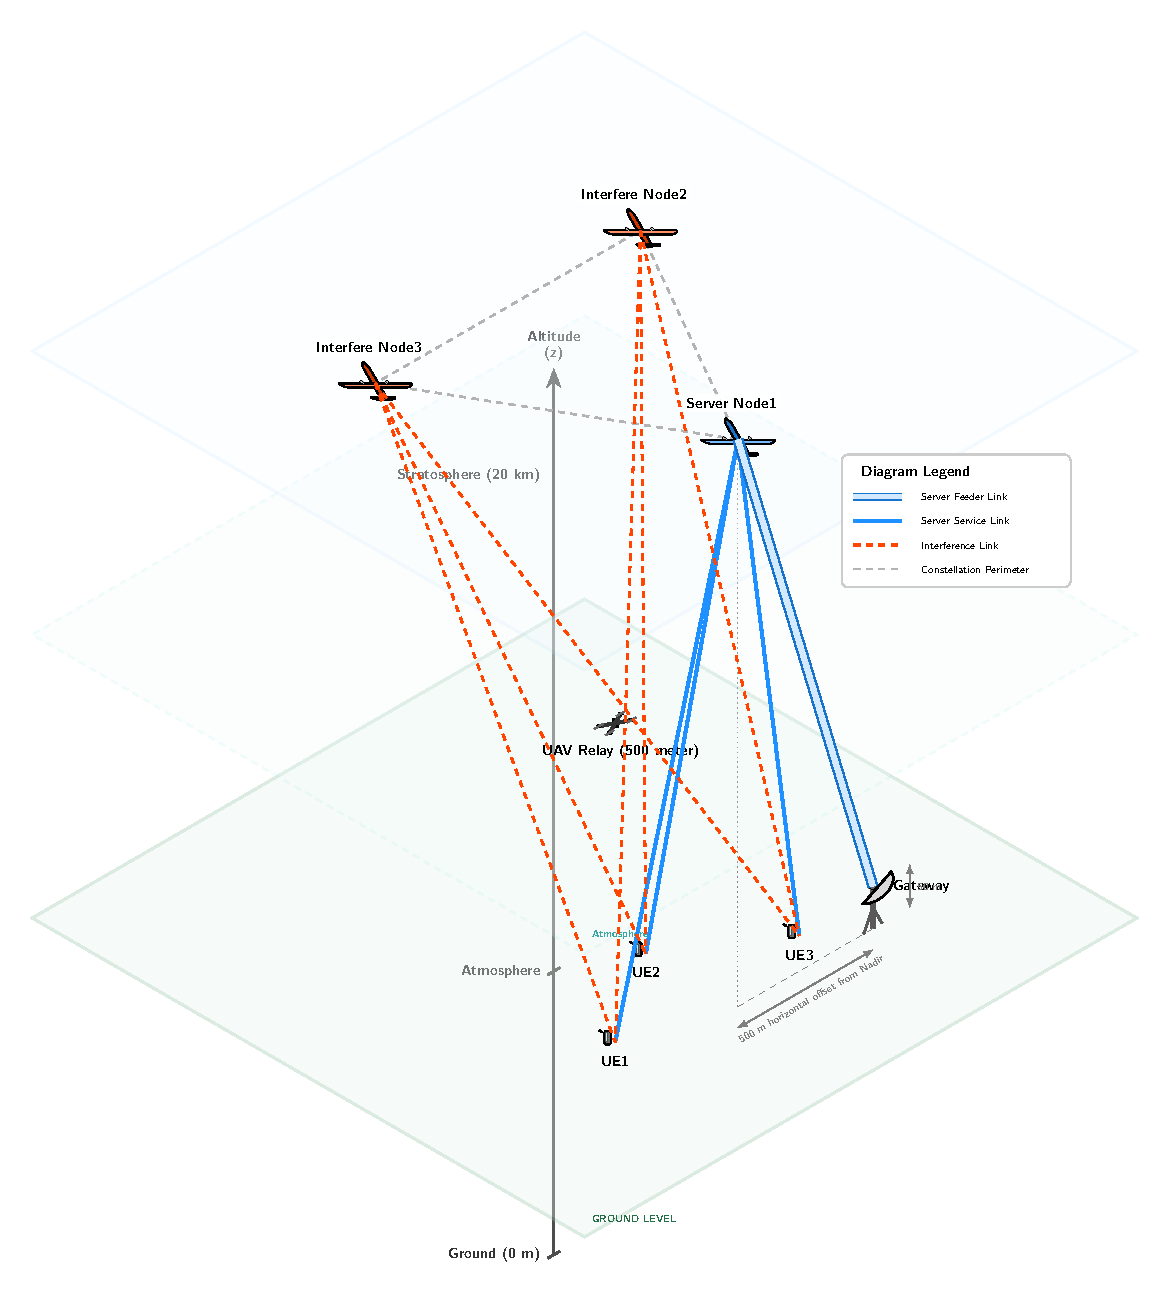
\includegraphics[width=0.9\linewidth]{./figures/network_diagram.pdf}
\caption{Topology}
\label{fig:simulation-topology}
\end{figure}

\subsection{Backhaul Link Geometry}
\label{subsec:backhaul-geometry}
Backhaul links operate in the 38.0–39.5 GHz millimeter-wave band allocated to HAPS at WRC-19 (Ka-band)~\cite{wrc19}.
The backhaul link is a short-range connection from the HAPS aircraft to the ground-based Gateway.
\begin{itemize}
  \item Gateway Altitude: 50 m AGL
  \item Altitude difference: $20\,\mathrm{km} - 0.05\,\mathrm{km} = 19.95\,\mathrm{km}$
  \item Horizontal distance: $50\,\mathrm{m}$ from HAPS nadir.
  \item Elevation angle: $\theta = \arctan\left(\frac{19.95}{0.05}\right) \approx 89.86^\circ$ (near zenith)
  \item Slant path: $L_{\text{slant}} = \sqrt{19.95^2 + 0.05^2} \approx 19.95\,\mathrm{km}$
  \item HAPS transmit power: $P_h = 43$\,dBm; HAPS-side transmit antenna gain: $G_h = 13.8$\,dBi (directional Ka-band aperture toward the Gateway, per the 30\,GHz-class HAPS link budget of Karaman et al.~\cite{karaman2025haps})
  \item Gateway receive antenna gain: $G_g = 39.7$\,dBi (fixed VSAT-class terminal, larger aperture feasible at a ground installation~\cite{karaman2025haps})
  \item Combined link EIRP + receive gain: $P_h + G_h + G_g \approx 96.5$\,dBm-equivalent, before FSPL and atmospheric losses (\S III.B)
\end{itemize}

\subsection{Relay Link Geometry}

The relay link (HAPS-to-UAV 38.0–39.5 GHz and UAV-to-User, f = 2.1 -- 2.2 GHz~\cite{wrc19,3gpp_ts38101_5}) connects HAPS to ground users via the UAV relay node positioned at
500 m AGL (Table~\ref{tab:config}).
\subsubsection{HAPS-to-UAV leg (Feeder Link, 38 GHz)}
\begin{itemize}
  \item UAV Relay Altitude: 500 m AGL
  \item Altitude difference: $20\,\mathrm{km} - 0.5\,\mathrm{km} = 19.5\,\mathrm{km}$
  \item Horizontal distance: $500\,\mathrm{m}$ from HAPS nadir.
  \item Elevation angle: $\theta = \arctan\left(\frac{19.5}{0.5}\right) \approx 88.5^\circ$ (near zenith)
  \item Slant path: $L_{\text{slant}} = \sqrt{19.5^2 + 0.5^2} \approx 19.51\,\mathrm{km}$
  \item HAPS transmit power: $P_h = 43$\,dBm; HAPS-side transmit antenna gain: $G_h = 13.8$\,dBi (same directional Ka-band aperture as the backhaul link, \S\ref{subsec:backhaul-geometry})
  \item UAV receive antenna gain: $G_u = 30.7$\,dBi (UAV-mountable 32$\times$32-element mmWave patch array, conservative low end of the 30.7--32.8\,dBi range reported at 25.4--26.9\,GHz~\cite{anim2021uav}, applied here at 38\,GHz)
\end{itemize}

\subsubsection{UAV-to-User leg (2.1 -- 2.2 GHz)}
\begin{itemize}
  \item User Altitude: 1.5 m (hand-held)
  \item Altitude difference: $0.5\,\mathrm{km} - 0.0015\,\mathrm{km} = 0.4985\,\mathrm{km}$
  \item Horizontal distance: $500\,\mathrm{m}$ to $100\,\mathrm{km}$ from UAV.
  \item Elevation angle: For 500m horizontal distance from UAV, $\theta = \arctan\left(\frac{0.4985}{0.5}\right) \approx 44.9^\circ$, for larger distances, the angle becomes much smaller.
  \item Slant path: $L_{\text{slant}} = \sqrt{0.4985^2 + 0.5^2} \approx 0.707\,\mathrm{km}$
  \item UAV transmit power: $P_u = 24$\,dBm; no directional antenna gain is modeled on this leg (UAV-side and UE-side antennas are treated as isotropic, consistent with the service link).
\end{itemize}

The second leg of relay link is dominated by
horizontal distance and building blockage rather than altitude. The attenuation grows sharply once
the horizontal offset exceeds the LoS-to-NLoS transition set by local building density and
built-up ratio (\S III.C, Eq.~\eqref{eq:los}--\eqref{eq:losJ}). This is why the UAV relay's
placement -- altitude and horizontal offset from served users -- depends on local landscape/building statistics. .

\subsection{Service Link Geometry}

Service links operate in the 2.1 -- 2.2 GHz  GHz FDD band (S-band)~\cite{3gpp_ts38101_5}. Service link connects
ground users directly to a HAPS serving node at 20 km altitude via a slant path extending up to the $\sim$100 km
service radius. Although the service link shares the 2 GHz band with the relay link, its power budget
 must close over a much longer range with a mostly-unobstructed, near-zenith-dominated geometry.
\begin{itemize}
  \item HAPS transmit power: $P_h = 43$\,dBm (same platform transmitter as the backhaul and feeder links; \texttt{P\_TX\_HAPS\_DBM}).
  \item No directional antenna gain is modeled on the service link (HAPS-side and UE-side antennas are treated as isotropic); unlike the 38\,GHz backhaul/feeder links, the service link's wide-area, long-range coverage requirement is not compatible with a narrow, high-gain beam.
\end{itemize}

% =====================================================================
\section{System and Channel Model}
% =====================================================================

This section presents three channel models for HAPS to Ground Scenario: (A) generic propagation formulae applicable to all frequency bands, (B) the 38 GHz backhaul link model (also reused for the 38 GHz feeder link, HAPS-to-UAV, in \S\ref{sec:relay-path-analysis}), and (C) the 2 GHz service/relay link model and finally

% =====================================================================
\subsection{Common System Models (All Frequency Bands)}
% =====================================================================

\subsubsection{Free-Space Path Loss~\cite{itu_p530}}
FSPL is calculated on the basis of a 20 km vertical zenith distance and a lateral reach extending to 100 km.
The ITU-R P.530~\cite{itu_p530} free-space path loss formula FSPL(MHz, km) is defined as
\begin{equation}
L_\mathrm{FSPL} = 32.44 + 20\log_{10} f_\mathrm{MHz} + 20\log_{10} d_\mathrm{km} \;[\mathrm{dB}].
\label{eq:fspl}
\end{equation}
$f_\mathrm{MHz}$ is the frequency of the HAPS carrier in MHz and $d_\mathrm{km}$ is the distance in km. This formula applies for all frequencies and distances in the HAPS service footprint, establishing the baseline attenuation before atmospheric and propagation effects. Used in the backhaul-link (38 GHz, §III.B) and service-link (2 GHz, §III.C) budgets, and reused for the feeder link (HAPS-to-UAV, 38 GHz, §\ref{sec:relay-path-analysis}). This is algebraically the same free-space loss as the wavelength form $L_\mathrm{FSPL}(h,g)=20\log_{10}(4\pi d_{h,g}/\lambda)$ used later in the multi-HAPS SINR derivation (Eq.~\eqref{eq:general-haps-sinr} et seq., \S III.D): substituting $\lambda=c/f$ and converting to MHz/km units folds the resulting constant $20\log_{10}(4\pi\times10^9/c)$ into the $32.44$\,dB term above.

% =====================================================================
\subsection{38 GHz Backhaul Link Model (HAPS-to-Gateway)}
% =====================================================================

The backhaul link (HAPS to Ground Gateway, 38--39.5 GHz Ka-band allocated at WRC-19). This path is vulnerable to atmospheric attenuation from rain, fog, gas absorption, and scintillation. Section III.B models each component sequentially; the same model is reused for the feeder link (HAPS-to-UAV, also 38--39.5 GHz) in \S\ref{sec:relay-path-analysis}.

\subsubsection{Specific Rain Attenuation~\cite{itu_p838}}
Rain attenuation $\gamma_R$ (dB/km) is calculated from the local rain
rate $R$ (mm/h) using the empirical ITU-R P.838 coefficients~\cite{itu_p838} $k,\alpha$:
\begin{equation}
\gamma_R = k(f,\theta) \; R^{\alpha(f,\theta)} \quad [\mathrm{dB/km}],
\label{eq:rain_spec_atten}
\end{equation}

For 38 GHz and $11.3^\circ$ elevation, the horizontal-polarisation coefficients computed with the \texttt{itur} implementation of ITU-R P.838 are $k\approx0.400$ and $\alpha\approx0.881$, giving $\gamma_R\approx3.04$\,dB/km at 10\,mm/h and $\approx6.82$\,dB/km at 25\,mm/h~\cite{itu_p838}. These values represent the power-law relationship between rain rate and specific attenuation.

When we multiply the effective path length $L_\mathrm{eff}$ (km) by this, we
obtain the rain loss:
\begin{equation}
A_\mathrm{rain} = \gamma_R \; L_\mathrm{eff} \quad [\mathrm{dB}],
\label{eq:rain_loss}
\end{equation}

\subsubsection{Total Rain Attenuation~\cite{itu_p618}}
The effective path length $L_\mathrm{eff}$ follows ITU-R P.618~\cite{itu_p618} (slant-path reduction factors and
site-dependent scaling for non-uniform rain along the path). The specific attenuation above is reported directly: for the 38\,GHz, $11.3^\circ$ worst-case backhaul path (102\,km slant), $\gamma_R\approx3.0$\,dB/km at 10\,mm/h and $\approx6.8$\,dB/km at 25\,mm/h. Multiplying by $L_\mathrm{eff}$ gives the path attenuation for a given rain rate. For the gateway geometry (89.86\,$^\circ$, 5.2\,km of rain), the path attenuation at a given rate is $\gamma_R L_s r$, where $L_s$ is the slant length through the rain layer and $r$ is the P.618 reduction factor. For Delhi, the ITU-R P.837 rain rate exceeded 0.1\,\% of the time is $R_{0.1}=15.7$\,mm/h, which gives $\approx19$\,dB of rain loss on the gateway path. The clear-sky gateway SNR is about 46\,dB, so after rain at 0.1\,\% about 27\,dB remains. The gaseous loss on the gateway path is $\approx0.4$\,dB (ITU-R P.676, $\rho=10$\,g/m$^3$), leaving about 26\,dB. The 38\,GHz gateway link therefore closes at 99.9\,\% availability. The 0.01\,\% rate ($R_{0.01}=61.8$\,mm/h) would give $\approx56$\,dB and is not the design target.

\subsubsection{Fog/Cloud Attenuation~\cite{itu_p840}}
Fog attenuation depends on the liquid-water density $M$ [g/m$^3$], frequency
$f$, and temperature $T$ per ITU-R P.840~\cite{itu_p840}. It is negligible below about 10 GHz, becomes noticeable
in the millimeter-wave bands, and can be several dB in dense fog.
Typical values are approximately 0.05 g/m$^3$ for medium fog and 0.5 g/m$^3$ for
dense fog~\cite{itu_p840}.
Cloud/fog attenuation is modeled as a specific attenuation $\gamma_c$ (dB/km)
times the slant-path length $L_\mathrm{slant}$ (km):
\begin{equation}
A_\mathrm{cloud} = \gamma_c(f,M,T) \;L_\mathrm{slant} \quad [\mathrm{dB}],
\label{eq:fog_loss}
\end{equation}

where $\gamma_c$ depends on the liquid-water density $M$ [g/m$^3$], frequency
and, weakly, on temperature. Typical liquid-water densities are $M\approx0.05$ for
medium fog and $M\approx0.5$ for dense fog; $\gamma_c$ is small below 10 GHz and
grows into the millimeter-wave bands~\cite{itu_p840}. For the 38 GHz backhaul link,
fog contributes negligibly to total loss (typically $<$0.2 dB).

\subsubsection{Atmospheric Gas Absorption~\cite{itu_p676}}
Atmospheric gas attenuation combines oxygen and water-vapour specific
attenuations $\gamma_o$ and $\gamma_w$ (dB/km) computed from
local pressure $p$, temperature $T$ and water-vapour density $\rho_w$ according to ITU-R P.676~\cite{itu_p676}.
The total gas loss is
\begin{equation}
A_\mathrm{gas} = (\gamma_o(p,T,f) + \gamma_w(\rho_w,T,f))\;L_\mathrm{slant} \quad [\mathrm{dB}],
\label{eq:gas_loss}
\end{equation}

Combines oxygen and water-vapor components according to ITU-R P.676 Sections 3.1 and 3.2~\cite{itu_p676}. The strongest absorption lines occur at 22.235 GHz and 183 GHz for water
vapor, and near 59.8 GHz and 118.75 GHz for oxygen~\cite{itu_p676} (P.676 Sect. 3.1--3.2, Figure 2).
This makes Ka/Q/V-band HAPS backhaul/feeder bands much more sensitive to moisture than the sub-6 GHz access links.
At 38 GHz, clear-sky gas absorption is approximately 0.2--0.3 dB/km, orders of magnitude lower than
at the 60 GHz oxygen resonance ($\sim$15--20 dB/km), justifying the 38 GHz band choice per ITU-R analysis~\cite{itu_p676}.

\subsubsection{Scintillation Fade Depth~\cite{itu_p618}}
Tropospheric scintillation refers to rapid fluctuations in signal amplitude and
phase caused by small-scale refractive-index irregularities in the lower
troposphere per ITU-R P.618~\cite{itu_p618}. In Ka-band (around 38 GHz) backhaul/feeder links, scintillation can cause
dynamic fading even in clear-sky conditions and must be taken into account when
designing beam-tracking and link-budget fade allowances~\cite{itu_p618}.

The fade depth due to scintillation for a specific time percentage $p$ is
commonly expressed as short-term amplitude fluctuations using the time percentage model (ITU-R P.618, Annex 1~\cite{itu_p618}):
\begin{equation}
A_\mathrm{scint}(p) = a(p) \cdot \sigma_{pre}(f,\theta,\mathrm{climate}) \quad [\mathrm{dB}],
\label{eq:scint_loss}
\end{equation}

where $a(p)$ maps standard-deviation values to time-percentage fades (ITU-R P.618 Annex 1~\cite{itu_p618})
and $\sigma_{pre}$ is calculated from the frequency, elevation angle $\theta$ and
local turbulence parameters in the recommendation. We then scale by $a(p)$ to obtain fade depths
for availability analyses and fade-allowance setting in adaptive systems. For 38 GHz at 11.3$^\circ$ elevation
and 0.01% outage, typical scintillation fade is 2--4 dB~\cite{itu_p618}.

So total slant-path attenuation for a backhaul link may be written as
\begin{equation}
L_\mathrm{total} = L_\mathrm{FSPL} + A_\mathrm{rain} + A_\mathrm{cloud/fog}
                  + A_\mathrm{gas} + A_\mathrm{scintillation},
\label{eq:feeder_loss}
\end{equation}

\subsubsection{Total Backhaul Link Attenuation~\cite{itu_p618}}
This equation sums all atmospheric and propagation effects (Eqs.~\eqref{eq:fspl}--\eqref{eq:scint_loss}) to compute the worst-case link budget for the HAPS-to-Gateway backhaul at 38 GHz. The breakdown is: FSPL (Eq.~\eqref{eq:fspl}) + rain (Eq.~\eqref{eq:rain_loss}) + fog (Eq.~\eqref{eq:fog_loss}) + gas (Eq.~\eqref{eq:gas_loss}) + scintillation (Eq.~\eqref{eq:scint_loss}), per ITU-R P.618 design guidance~\cite{itu_p618}.

\begin{table}[t]
\centering
\caption{Atmospheric Effects and ITU-R Recommendations for HAPS backhaul/feeder links (38 GHz)}
\label{tab:atmospheric_effects}
{\scriptsize\setlength{\tabcolsep}{3pt}
\begin{tabularx}{\columnwidth}{|>{\raggedright\arraybackslash}p{0.27\columnwidth}|>{\raggedright\arraybackslash}p{0.16\columnwidth}|>{\raggedright\arraybackslash}X|}
\hline
\textbf{Atmospheric Effect} & \textbf{Affected Frequency} & \textbf{ITU Recommendation}  \\
\hline
Rain attenuation & $>$1 GHz & ITU-R P.618 (Earth–space path prediction), P.837 (rain climate statistics / rain rate), P.838 (specific attenuation)\\
\hline
Clouds and fog & 1--200 GHz & ITU-R P.840\\
\hline
Atmospheric gases (oxygen and water vapour) & 1--1000 GHz & ITU-R P.676\\
\hline
Atmospheric profiles (pressure, temperature, humidity) & all bands & ITU-R P.835\\
\hline
Surface water vapour statistics & all bands & ITU-R P.836\\
\hline
Tropospheric scintillation & 1--100 GHz & ITU-R P.618\\
\hline
\end{tabularx}}
\end{table}

% =====================================================================
\subsection{2 GHz Service/Relay Link Model (UAV-to-User Air-to-Ground)}
% =====================================================================

Service and relay links operate at 2--2.2 GHz (S-band per 3GPP TS 38.821), connecting ground users either directly to HAPS (service link, high elevation angle) or via UAV relays at 500 m altitude (relay link). Unlike the 38 GHz backhaul and feeder links, the 2 GHz S-band is resilient to atmospheric effects (fog, rain, gas absorption all negligible per ITU-R P.618) but highly sensitive to building blockage. This section models LoS probability, path loss, and multi-node interference.

\subsubsection{Building-Blockage LoS Probability~\cite{holispechac2008}}
For a UAV $u$ at horizontal distance $r_{u,k}$ from user $k$, the LoS
probability follows the exact building-blockage product series
of~\cite{arani2023}, which uses the building parameters of~\cite{holispechac2008} (IEEE Trans. Antennas Propag., 2008, vol. 56, no. 4, pp. 1078--1084):
\begin{equation}
P^\mathrm{LoS}_{u,k} = \prod_{n=0}^{J}\left[1-\exp\!\left(-\frac{1}{2\xi^2}
\Big(h_u-\tfrac{n+\frac12}{J+1}(h_u-h_k)\Big)^{2}\right)\right],
\label{eq:los}
\end{equation}

Product-series model~\cite{arani2023} for line-of-sight probability accounting for cumulative building blockage along the path. The product iterates over building layers from ground to UAV height.

\subsubsection{Number of Building Layers~\cite{holispechac2008}}
\begin{equation}
J = \left\lfloor \frac{r_{u,k}}{1000}\sqrt{\alpha\beta} - 1 \right\rfloor,
\label{eq:losJ}
\end{equation}

Computed from horizontal distance $r_{u,k}$ (meters), building density $\beta$ [buildings/km$^2$], and built-up ratio $\alpha$ [dimensionless] per Holis \& Pechac Table I~\cite{holispechac2008}.

\noindent Parameters from Table I (Holis \& Pechac 2008, IEEE Trans. Antennas Propag.~\cite{holispechac2008}): $P_\mathrm{NLoS}=1-P_\mathrm{LoS}$; $\alpha$ is the built-up land ratio,
$\beta$ the mean building density [buildings/km$^2$], and $\xi$ a building-height parameter [m]. All are
environment-dependent: for urban areas~\cite{holispechac2008},
$\alpha=0.3$, $\beta=500$, $\xi=15$\,m; dense urban uses $\alpha=0.5$, $\beta=300$, $\xi=20$\,m;
suburban $\alpha=0.1$, $\beta=750$, $\xi=8$\,m; high-rise $\alpha=0.5$, $\beta=300$, $\xi=50$\,m (Table I)~\cite{holispechac2008}.

\noindent\textbf{Landscape-based relay placement:} The LoS probability model above (Eq.~\eqref{eq:los}--\eqref{eq:losJ}), with its environment-dependent $\alpha,\beta,\xi$ parameter sets (urban, dense urban, suburban, high-rise), already provides the mechanism for determining where a UAV relay stays in LoS of its served users. This same mechanism determines the UAV relay's altitude and horizontal-offset placement per landscape, as introduced in \S II (Relay Link Geometry).

\noindent\textbf{Single-relay scope:} This document limits the topology to one UAV relay (Table~\ref{tab:config}), so the interference sum in the SINR expression (Eq.~\eqref{eq:sinr}, generalized as Eq.~\eqref{eq:spatial-sinr}) need only account for the 3 HAPS for the relay link -- no UAV-to-UAV (relay-to-relay) interference term is needed.

\subsubsection{Probability-Averaged Path Loss}
Unlike terrestrial base stations, HAPS nodes operate at high elevation angles. This near-zenith positioning provides a superior Line-of-Sight (LoS) probability, significantly reducing multi-path fading and shadowing in urban and mountainous terrain.
Each state $z\in\{\mathrm{LoS},\mathrm{NLoS}\}$ adds an additional shadowing loss $X_z$ in dB:
the LoS term is zero-mean log-normal with $\sigma_\mathrm{LoS}=4$\,dB (midpoint of the 3--5\,dB range in
Holis \& Pechac~\cite{holispechac2008}); the NLoS term has mean $\mu(\theta)$ and standard deviation $\sigma(\theta)$
from their Eq.~(4) and Table~IV (2\,GHz, all environments), with $\theta$ the elevation of the UAV as seen from the user.
Because the shadowing is log-normal in linear gain, the states are averaged in linear gain, not in dB:
\begin{align}
\overline{g} &= 10^{-\mathrm{FSPL}/10}\Big[P_\mathrm{LoS}\,e^{\tfrac{(a\sigma_\mathrm{LoS})^2}{2}}
              + P_\mathrm{NLoS}\,e^{-a\mu(\theta)+\tfrac{(a\sigma(\theta))^2}{2}}\Big], \qquad a=\tfrac{\ln 10}{10},\\
\overline{\mathrm{PL}} &= -10\log_{10}\overline{g},
\label{eq:pl}
\end{align}
where $\mathrm{FSPL}=20\log_{10}(4\pi f d_\mathrm{3D}/c)$ and $P_\mathrm{LoS}$ is the LoS probability (Eq.~\eqref{eq:los}).
The 3D distance is $d_\mathrm{3D}=\sqrt{r^2+(h_u-h_k)^2}$ where $r$ is horizontal distance and $h_u, h_k$ are UAV and user altitudes.
At elevations where $P_\mathrm{LoS}$ is near 0 or 1 the linear and dB averages agree; in between they differ by up to about 17\,dB,
so the linear form is required for the expected received power.

The received power follows the standard link-budget relation
\begin{equation}
P_r = P_t + G_t + G_r - PL(d,\theta,\mathrm{state}),
\label{eq:rx-power}
\end{equation}
where $P_t$ is transmit power, $G_t$ and $G_r$ are the transmit and receive antenna gains, and $PL(d,\theta,\mathrm{state})$ is the path loss for the current geometry and propagation state. A blocked or NLoS link therefore yields a smaller $P_r$ through a larger path-loss term (equivalently, a lower channel gain $g_{u,k}$); it is not added as a separate degradation term in the SINR expression itself. The reduced signal power is already embedded in the SINR numerator before interference and noise are considered.

The downlink SINR is
\begin{equation}
\gamma_{u,k} = \frac{p_u\,g_{u,k}}{\sum_{u'\neq u} p_{u'} g_{u',k} + \sigma_0^2},
\qquad g_{u,k}=10^{-\overline{\mathrm{PL}}/10},
\label{eq:sinr}
\end{equation}

\subsubsection{Signal-to-Interference-plus-Noise Ratio (SINR)}
Computes downlink SINR at user $k$ from UAV $u$ per standard information-theory formulation. $p_u$ is transmit power [Watts], $g_{u,k}=10^{-\overline{\mathrm{PL}}/10}$ is channel gain (reciprocal of path loss in linear scale), interference sums over competing UAVs $u'$, and $\sigma_0^2$ is thermal noise power [Watts]. For the noise-limited characterization below, interference is negligible; the characterisation below is
noise-limited.

% =====================================================================
\section{Simulation and Results}
% =====================================================================

All numerical results in this section were generated with a Python simulation
stack: \texttt{NumPy}/\texttt{pandas} for the channel, battery, and association
models, and \texttt{Matplotlib} for figure generation. Atmospheric and
scintillation losses (rain, cloud/fog, gas, and ITU-R P.618 scintillation) are
computed with the \texttt{ITU-Rpy} (\texttt{itur}) library, which implements the
relevant ITU-R propagation recommendations directly rather than re-deriving
them by hand. The learned association policy (LSTM and DRL) (Section~\ref{sec:lstm-dqn-motivation})
uses a custom Deep Q-Network agent implemented in \texttt{PyTorch}
(\texttt{torch}/\texttt{torch.nn}), rather than a third-party RL library, trained
against the per-user association environment described above.

% =====================================================================
\subsection{Loss applicable to both frequencies}
% =====================================================================

\subsubsection{Free-space path loss}

Both 2 GHz and 38 GHz bands are governed by the same universal equations for free-space path loss (Eq.~\eqref{eq:fspl}).

\begin{figure}[h!]\centering
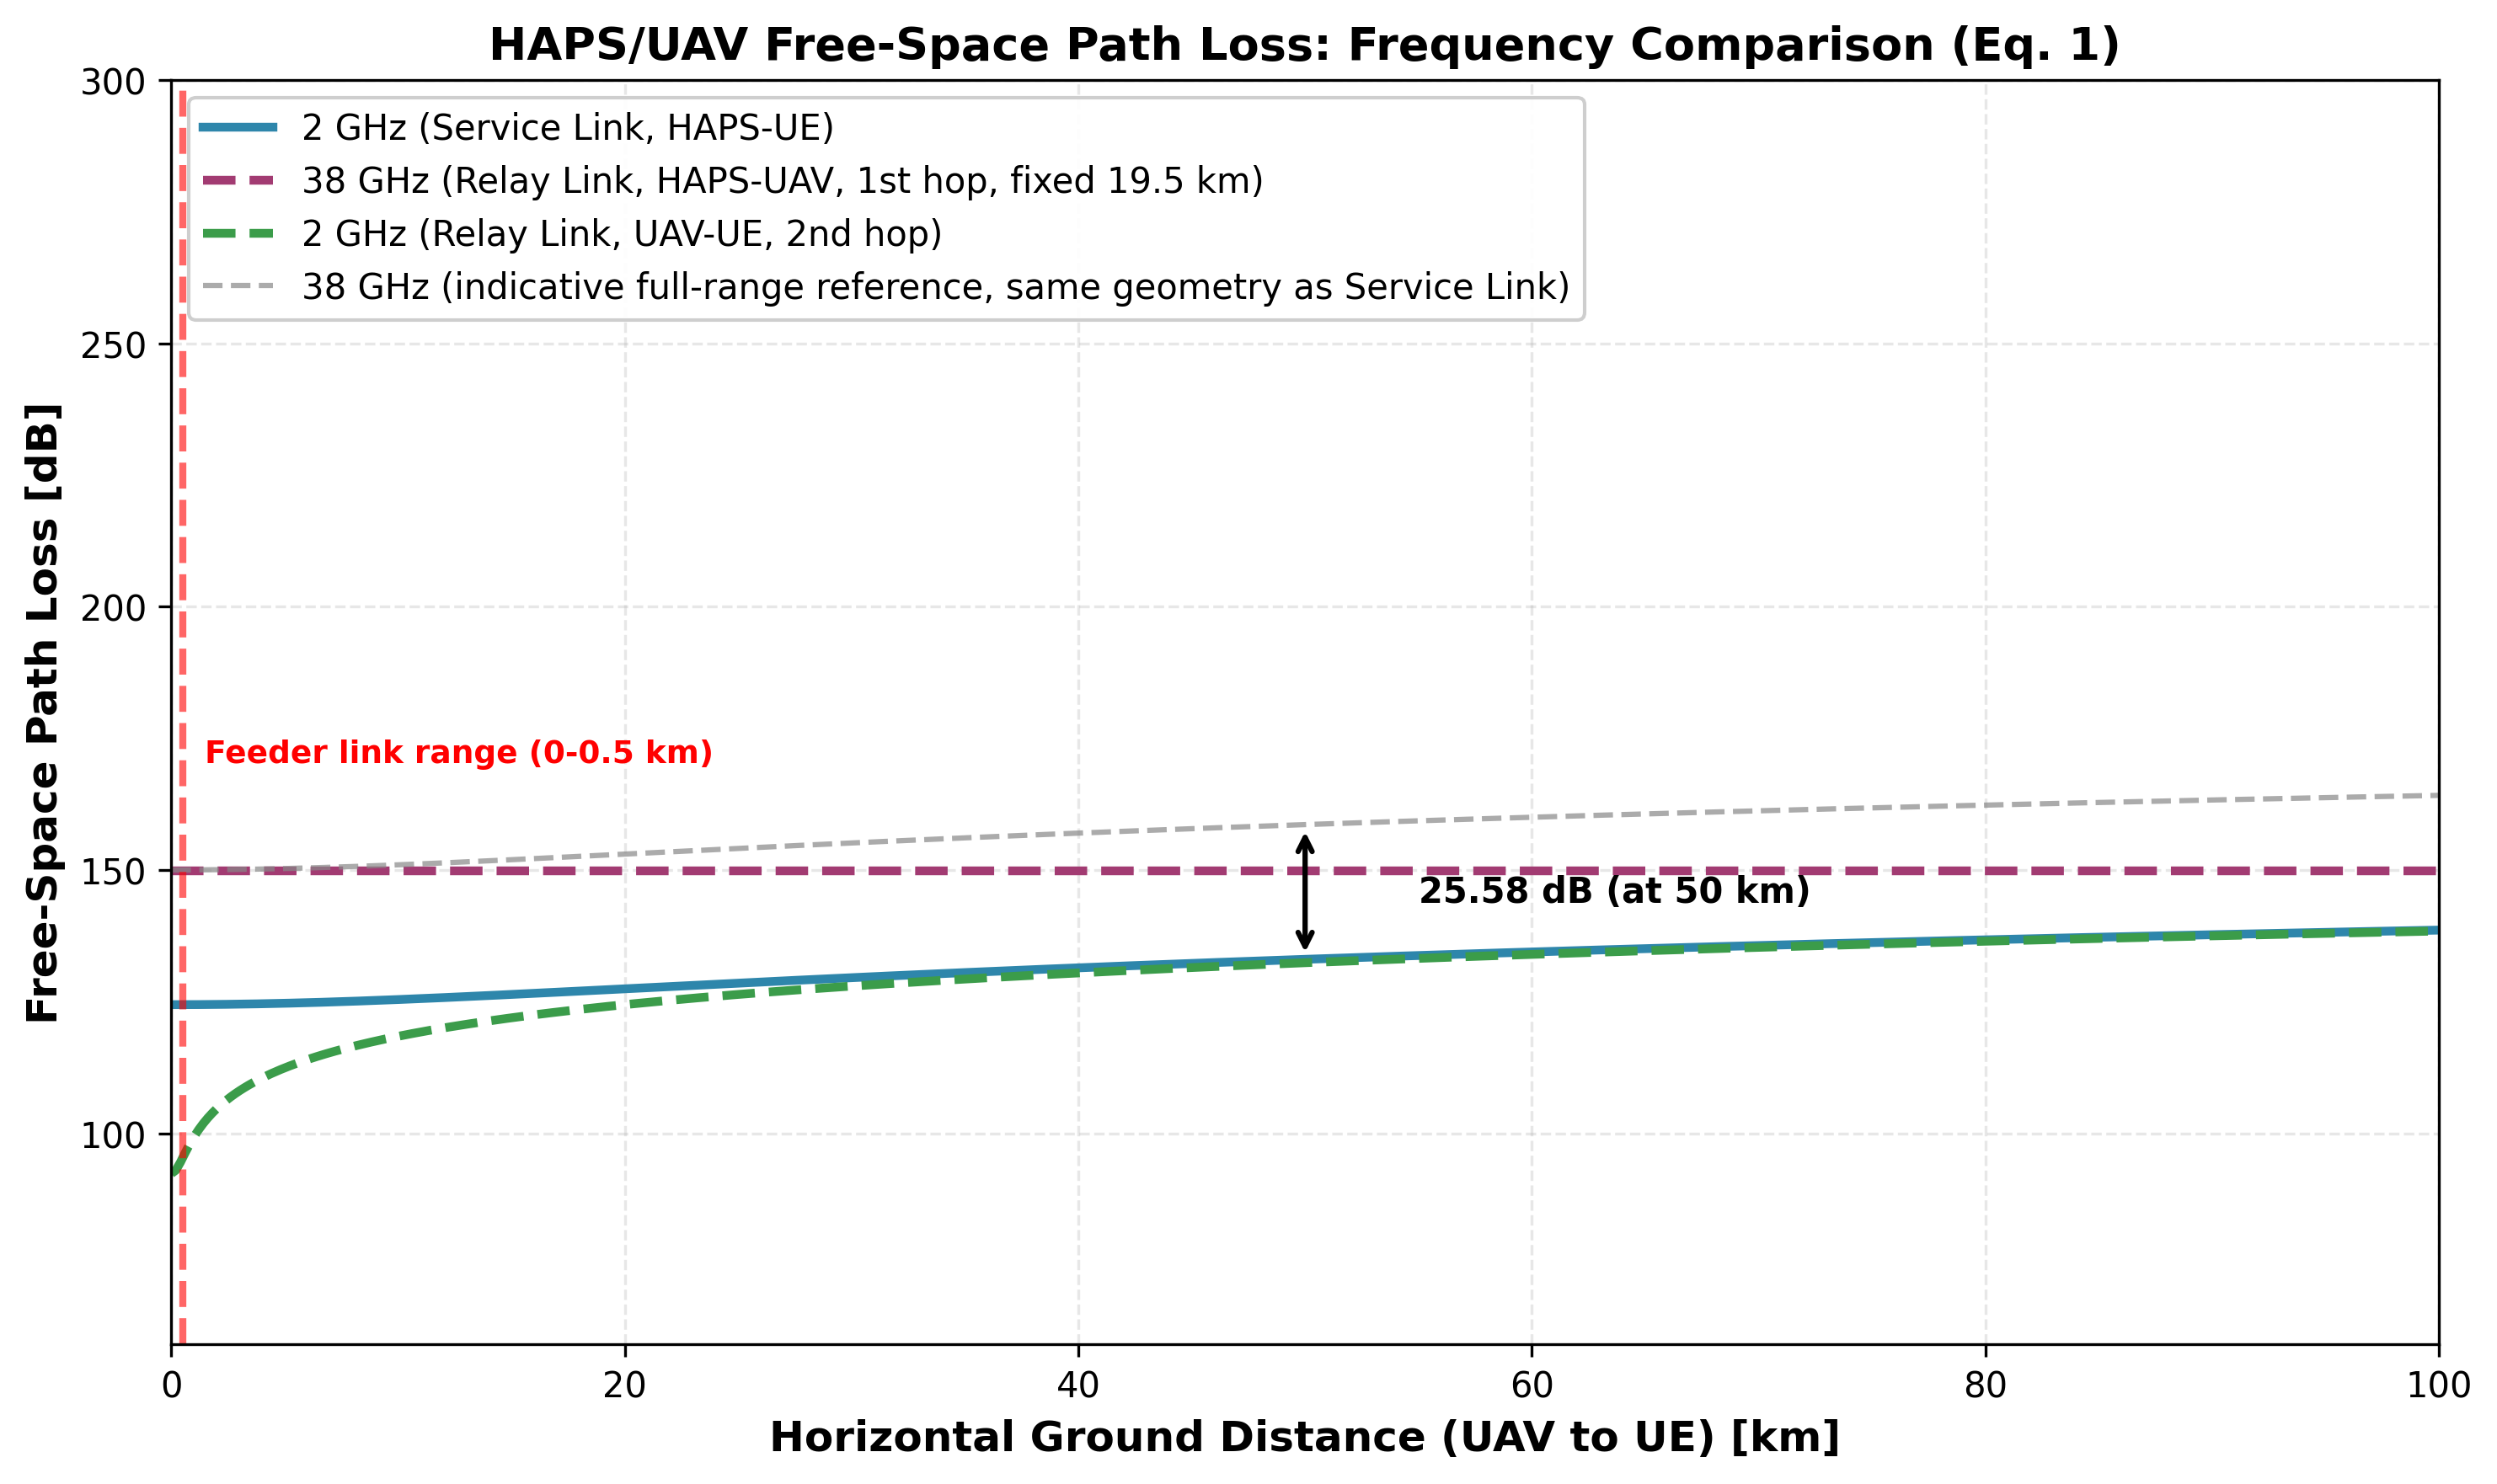
\includegraphics[width=0.95\columnwidth]{./figures/1b_haps_fspl_2ghz_vs_38ghz.png}
\caption{HAPS/UAV free-space path loss, \eqref{eq:fspl}, over a 0--100\,km horizontal footprint.}
\label{fig:fspl_comparison}
\end{figure}

In the above figure we can see the FSPL for the following paths,
\begin{itemize} 
\item {Solid blue} 2\,GHz service link (HAPS\textrightarrow UE).
\item {Dashed green} 2\,GHz relay link, 2nd hop (UAV\textrightarrow UE). 
\item {Dashed purple} 38\,GHz relay link, 1st hop (HAPS\textrightarrow UAV) 
                         this leg does not extend past the UAV; hence flat
\item {Dashed grey} 38\,GHz reference (HAPS\textrightarrow UE) for comparison only, no such direct link exists in the system model.
\end{itemize}
 
\textbf{Observations:}
\begin{itemize} 
\item  Every 10× increase in distance adds $20\log_{10}(10)=20\text{dB}$ path loss.
\item A constant \textbf{25.6\,dB offset} could be seen between 38 GHz and 2 GHz links $20\log_{10}(38/2)$. 
\item FSPL is per-hop; the hops are independent RF links and hence bottlenecked by the weaker hop (min of per-hop capacities).
\end{itemize}


\subsubsection{Scintillation fade depth}
\label{subsec:scintillation}

Tropospheric scintillation is rapid amplitude fluctuations caused by refractive-index turbulence in the lower atmosphere.
The fade $A_s(p)$, exceeded for $p$\% of the time, is computed with the ITU-R P.618 method (\texttt{itur}
implementation, scintillation attenuation) at the site 28.61\,N, 77.21\,E, with $T=15^\circ$\,C, relative humidity 60\,\%,
pressure 1010\,hPa and antenna efficiency $\eta=0.5$. The aperture is $D=0.31$\,m for the 38\,GHz gateway link (the working-set
gateway dish) and $D=1$\,m for the 2.1\,GHz link (a stated reference aperture). The table of $A_s(p)$ used in the model is:

\begin{center}
\resizebox{\columnwidth}{!}{%
\begin{tabular}{lcccc}
\toprule
 & \multicolumn{2}{c}{38\,GHz, $D=0.31$\,m} & \multicolumn{2}{c}{2.1\,GHz, $D=1$\,m} \\
Elevation & $p=0.01$\,\% & $p=1$\,\% & $p=0.01$\,\% & $p=1$\,\% \\
\midrule
$10^\circ$ & 1.76\,dB & 0.73\,dB & 0.33\,dB & 0.14\,dB \\
$30^\circ$ & 0.49\,dB & 0.21\,dB & 0.09\,dB & 0.04\,dB \\
$60^\circ$ & 0.25\,dB & 0.11\,dB & 0.05\,dB & 0.02\,dB \\
$89.86^\circ$ & 0.21\,dB & 0.09\,dB & 0.04\,dB & 0.02\,dB \\
\bottomrule
\end{tabular}}
\end{center}

The fade at $30^\circ$ is about 0.5\,dB at 38\,GHz and about 0.09\,dB at 2.1\,GHz for $p=0.01$\,\%. The fade grows with frequency and
with decreasing elevation, as the P.618 method predicts. The earlier empirical fit, with an exponent of 0.7 that was not
validated by measurement, is no longer used.

\begin{figure}[ht]\centering
\begin{subfigure}[b]{0.45\columnwidth}\centering
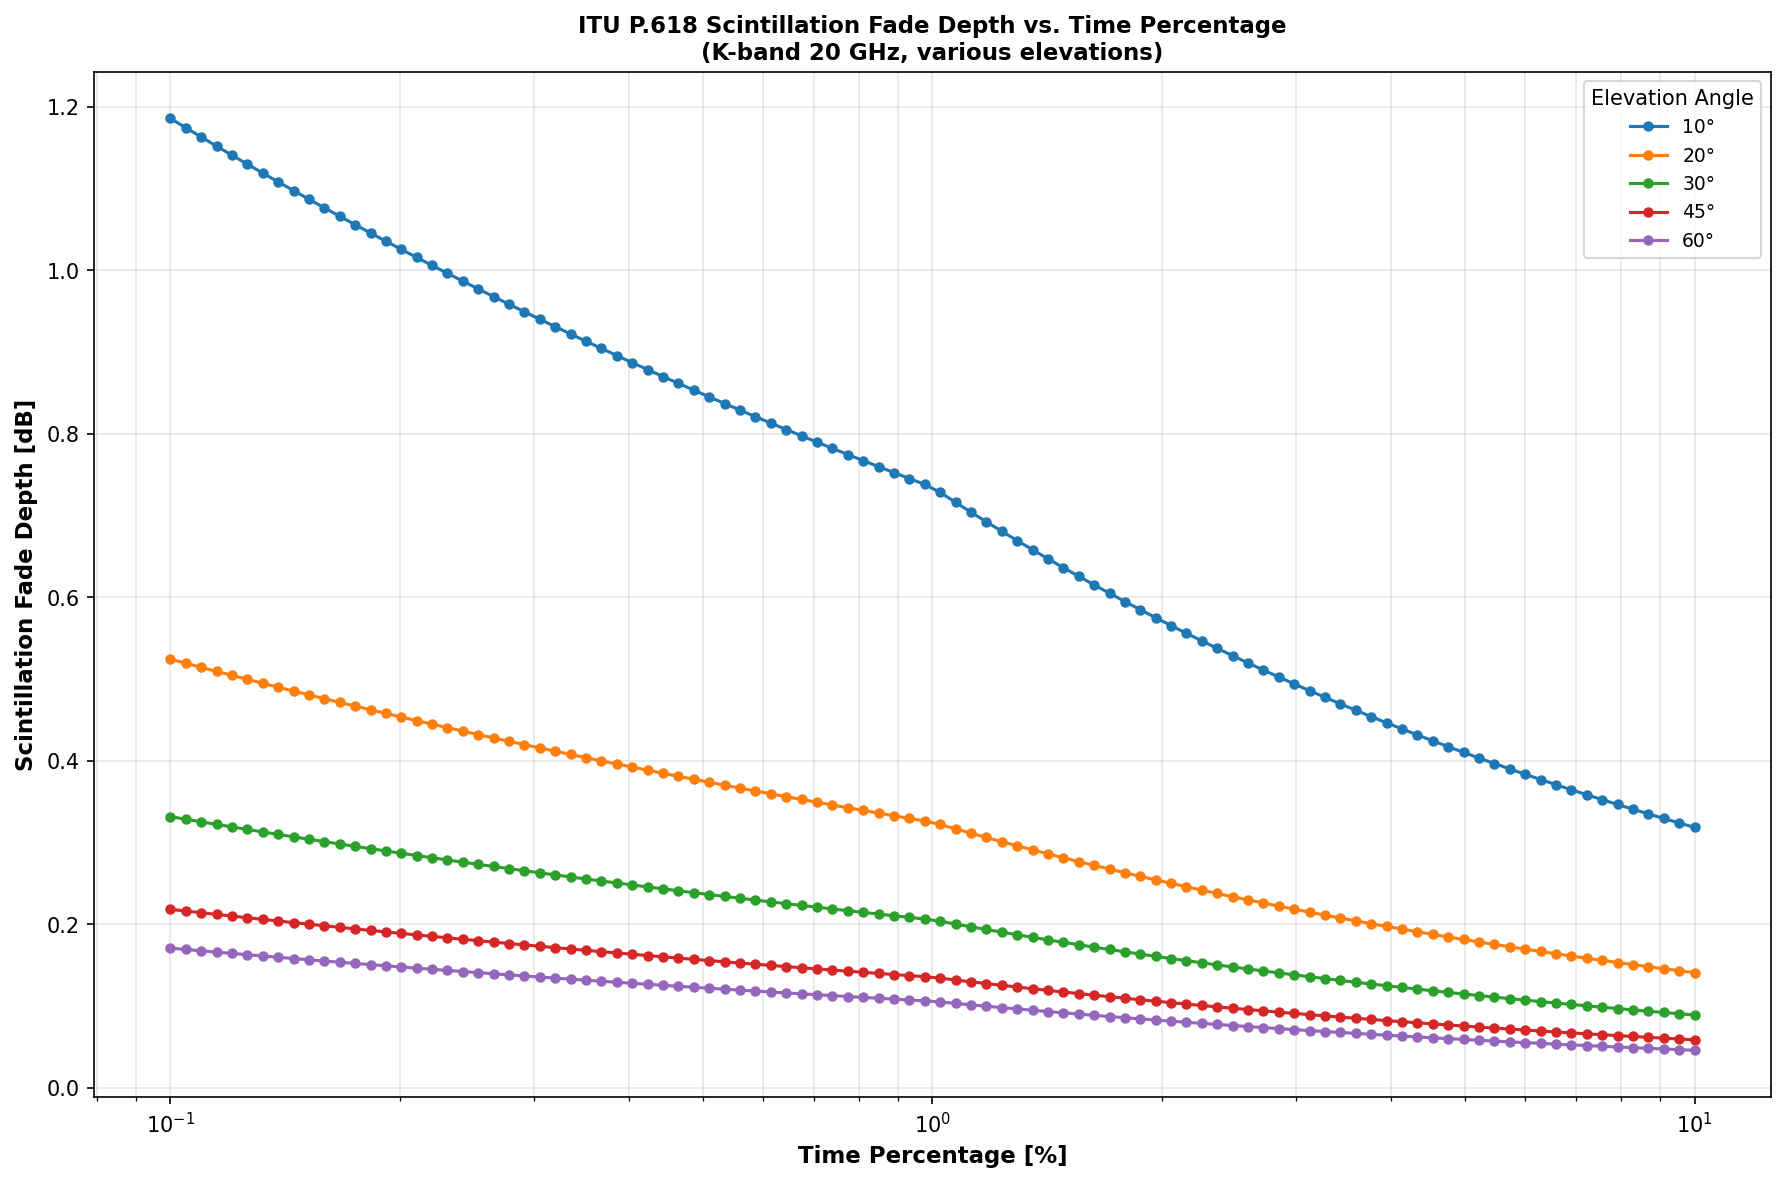
\includegraphics[width=0.95\textwidth]{./figures/9a_scintillation_fade_vs_time.png}
\caption*{(a) vs.\ time percentage}
\end{subfigure}
\hfill
\begin{subfigure}[b]{0.45\columnwidth}\centering
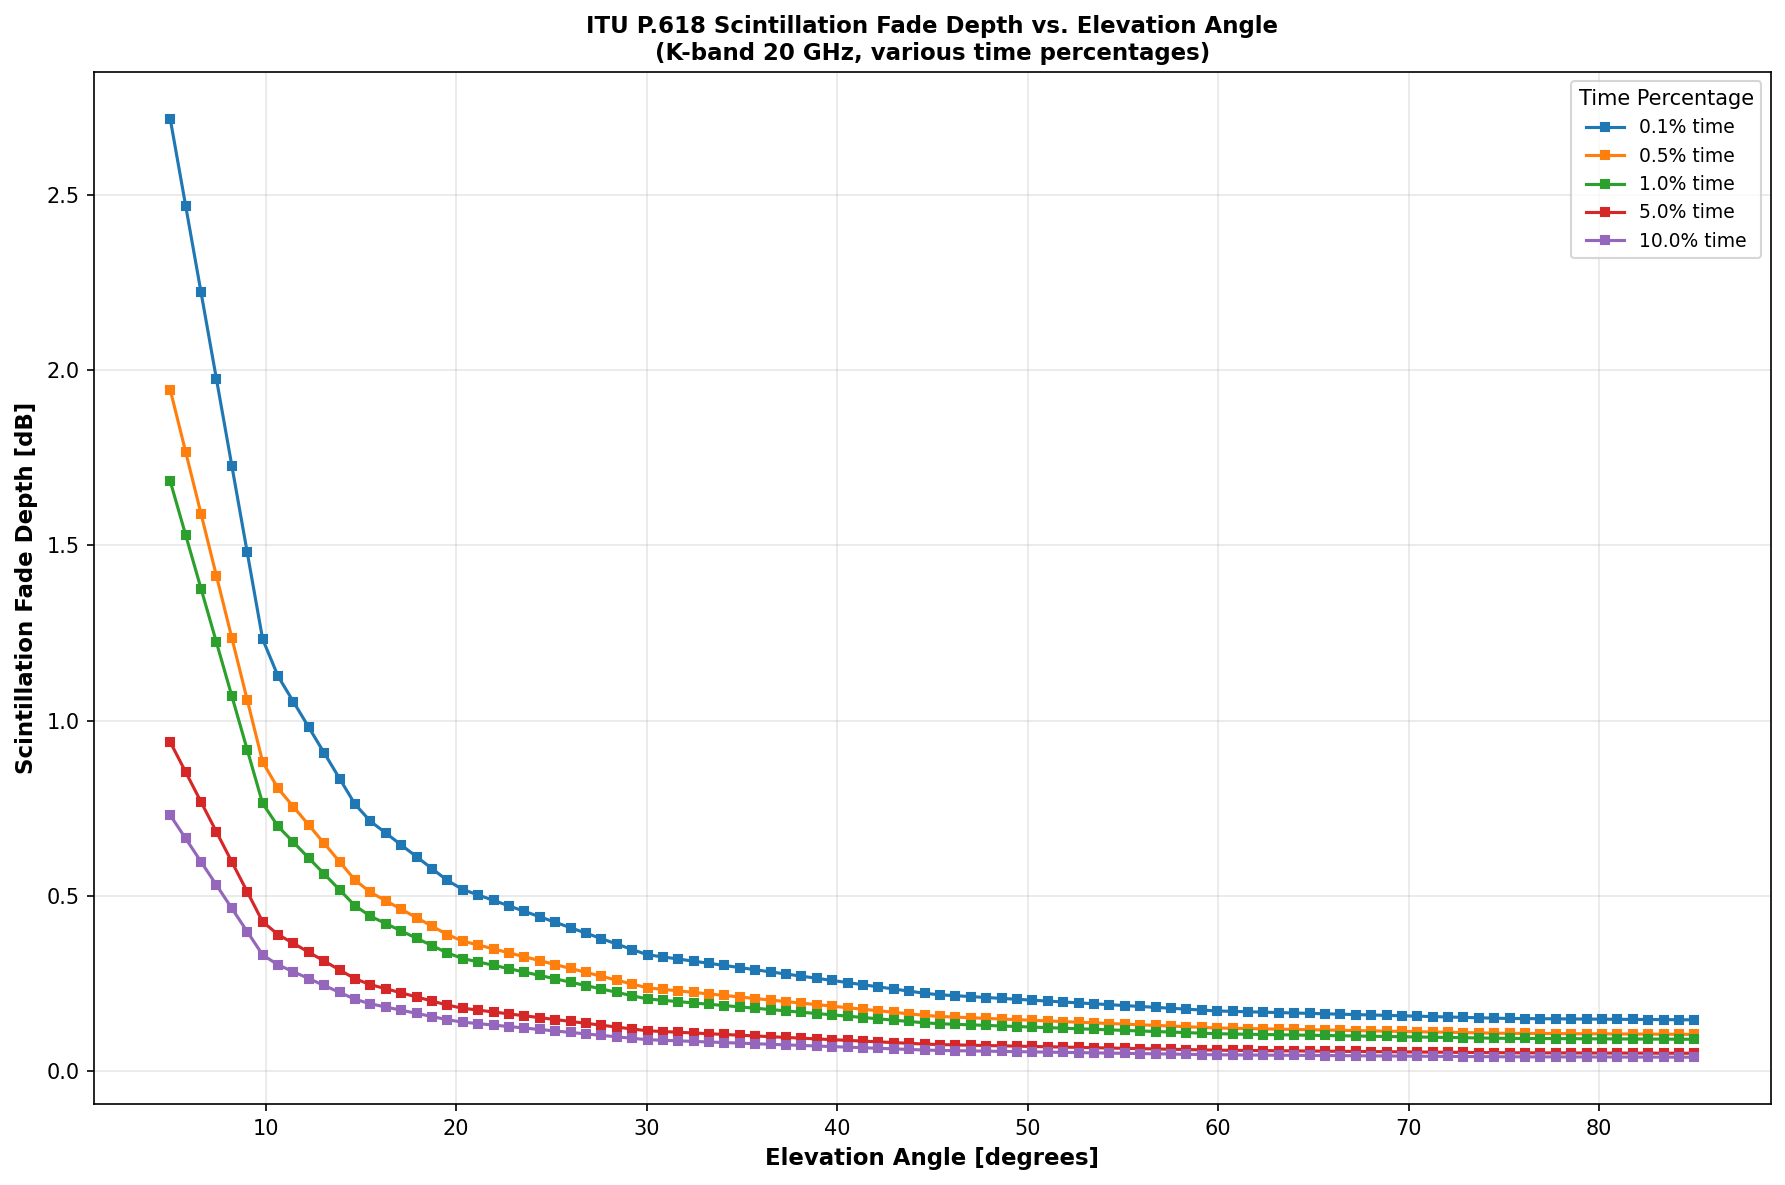
\includegraphics[width=0.95\textwidth]{./figures/9b_scintillation_fade_vs_elev.png}
\caption*{(b) vs.\ elevation}
\end{subfigure}
\caption{Scintillation fade depth characteristics (ITU-R P.618, \texttt{itur}, gateway geometry at 38\,GHz with $D=0.31$\,m and 2.1\,GHz with $D=1$\,m): \textbf{(a)} Fade depth vs.\ time percentage at five elevation angles ($10\circ$--$60\circ$). \textbf{(b)} Fade depth vs.\ elevation angle at four time percentages ($0.01\%$--$10\%$).}
\label{fig:scint_fade_depth}
\end{figure}

\textbf{Observations}: 
\begin{itemize}
  \item The backhaul/feeder links (38~GHz) carry a 25.6\,dB FSPL penalty as well as $8.95 \, \mathrm{dB}$ scintillation fade penalty.
  \item In general, the scintillation formula indicates fade depth increases with frequency, decreases with elevation angle.
  \item This favors positioning relay UAVs at higher elevation angles near the nadir when feasible, especially for the HAPS-UAV leg.
\end{itemize}

A Johnson--Nyquist thermal-noise model, $N=kTB$, or equivalently $N_{\text{dBm}}=-174+10\log_{10}(B)+NF$, would provide a more physically grounded noise estimate than the assumed flat $-100$\,dBm noise floor used elsewhere in this document. However, for short-range backhaul-link analysis, replacing the assumed noise floor with a bandwidth- and receiver-dependent thermal-noise value would primarily change the absolute SINR level rather than its trend with distance. A more detailed link-budget analysis incorporating the actual channel bandwidth, receiver noise figure, directional gateway antenna gain, and HAPS transmit power is deferred to the next phase.

% =====================================================================
\subsection{Loss specific to 2GHz band}
% =====================================================================

\subsubsection{SINR for different landscapes}

2-2.2~GHz S-band used in service and relays are resilient to atmospheric effects (fog, rain, gas absorption all negligible per ITU-R P.618) however they are highly sensitive to building blockage, the following chart shows the path loss with 2GHz links in different landscapes.

\begin{figure}[ht]\centering
\begin{subfigure}[b]{0.49\columnwidth}
\centering
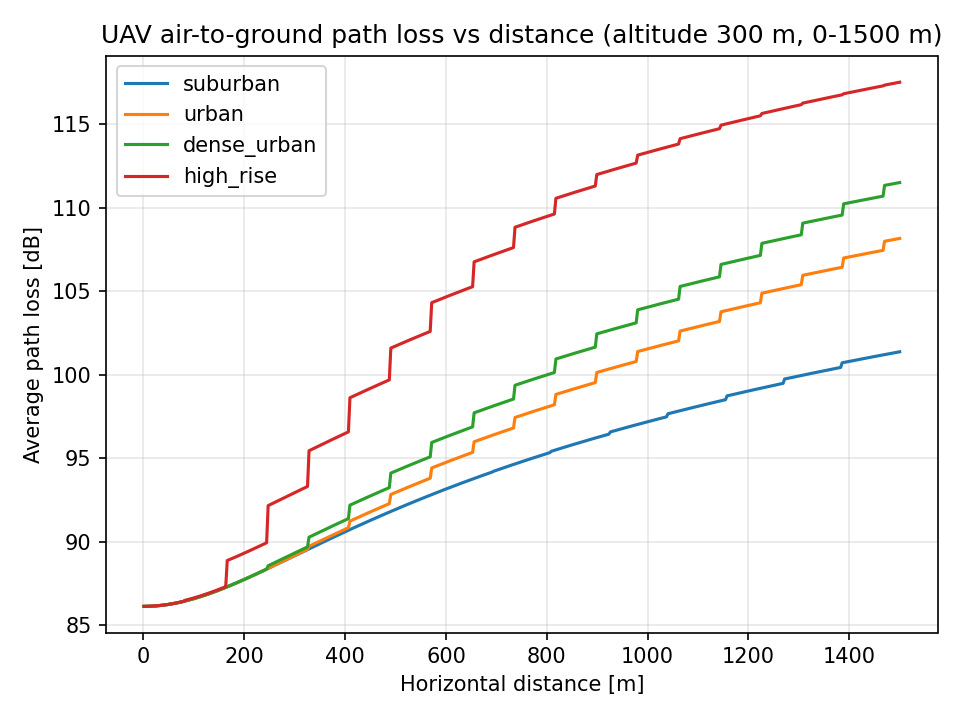
\includegraphics[width=\columnwidth]{./figures/3_uav_pathloss.png}
\caption*{(a) Path Loss}
\end{subfigure}
\begin{subfigure}[b]{0.49\columnwidth}
\centering
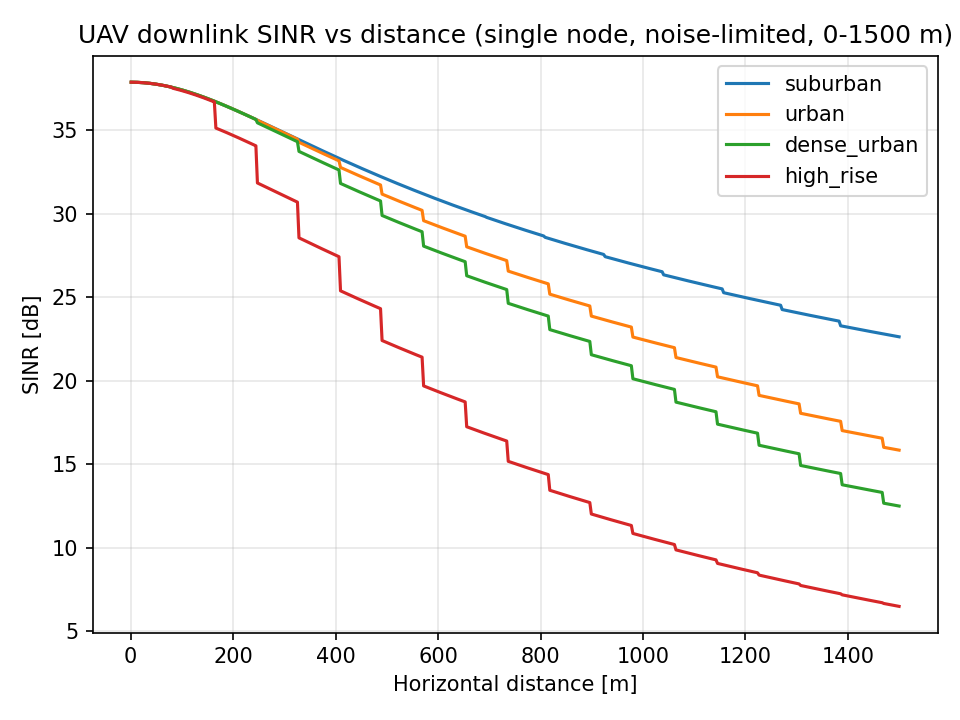
\includegraphics[width=\columnwidth]{./figures/4_sinr.png}
\caption*{(b) SINR}
\end{subfigure}
\caption{2~GHz service/relay link propagation (UAV altitude 500\,m)}
\label{fig:los_pl_sinr}
\end{figure}

\textbf{Observations}: 
\begin{itemize}
\item The Suburban landscape has lowest loss; 
\item High-rise landscape has higher blockage loss as well as sharp LoS/NLoS transitions.
\end{itemize}

% =====================================================================
\subsection{Loss specific to 38 GHz Band}
% =====================================================================

\subsubsection{Why 38 GHz instead of 2 GHz for the backhaul and feeder links}

At 38 GHz, $\lambda = 7.9$\,mm, and the antenna gains of the link budget (\S\ref{subsec:backhaul-geometry}) set the 3\,dB beamwidths $\theta \approx \sqrt{41253/G}$ (degrees, $G$ linear): about $2.1^\circ$ for the gateway dish ($G_g = 39.7$\,dBi, $\approx0.31$\,m aperture at $\eta\approx0.6$), about $5.9^\circ$ for the UAV array ($G_u = 30.7$\,dBi, $\approx0.11$\,m), and about $41^\circ$ for the HAPS ($G_h = 13.8$\,dBi, a small patch). These narrow beams enable point-to-point backhaul/feeder links with interference rejection. Also higher frequencies enable wider bandwidth (Ka-band supports 1+ GHz channels). Also ITU-R allocates 2 GHz (S-band) for \emph{terrestrial mobile access} (3GPP) and 38--39.5 GHz (Ka-band) for \emph{fixed HAPS backhaul} (WRC-19~\cite{wrc19}). However 38 GHz band presents specific challenges with atmospheric loss, rain attenuation, and scintillation. The following sections analyze the frequency effects on atmospheric loss in detail.
 
\begin{figure}[h!]\centering
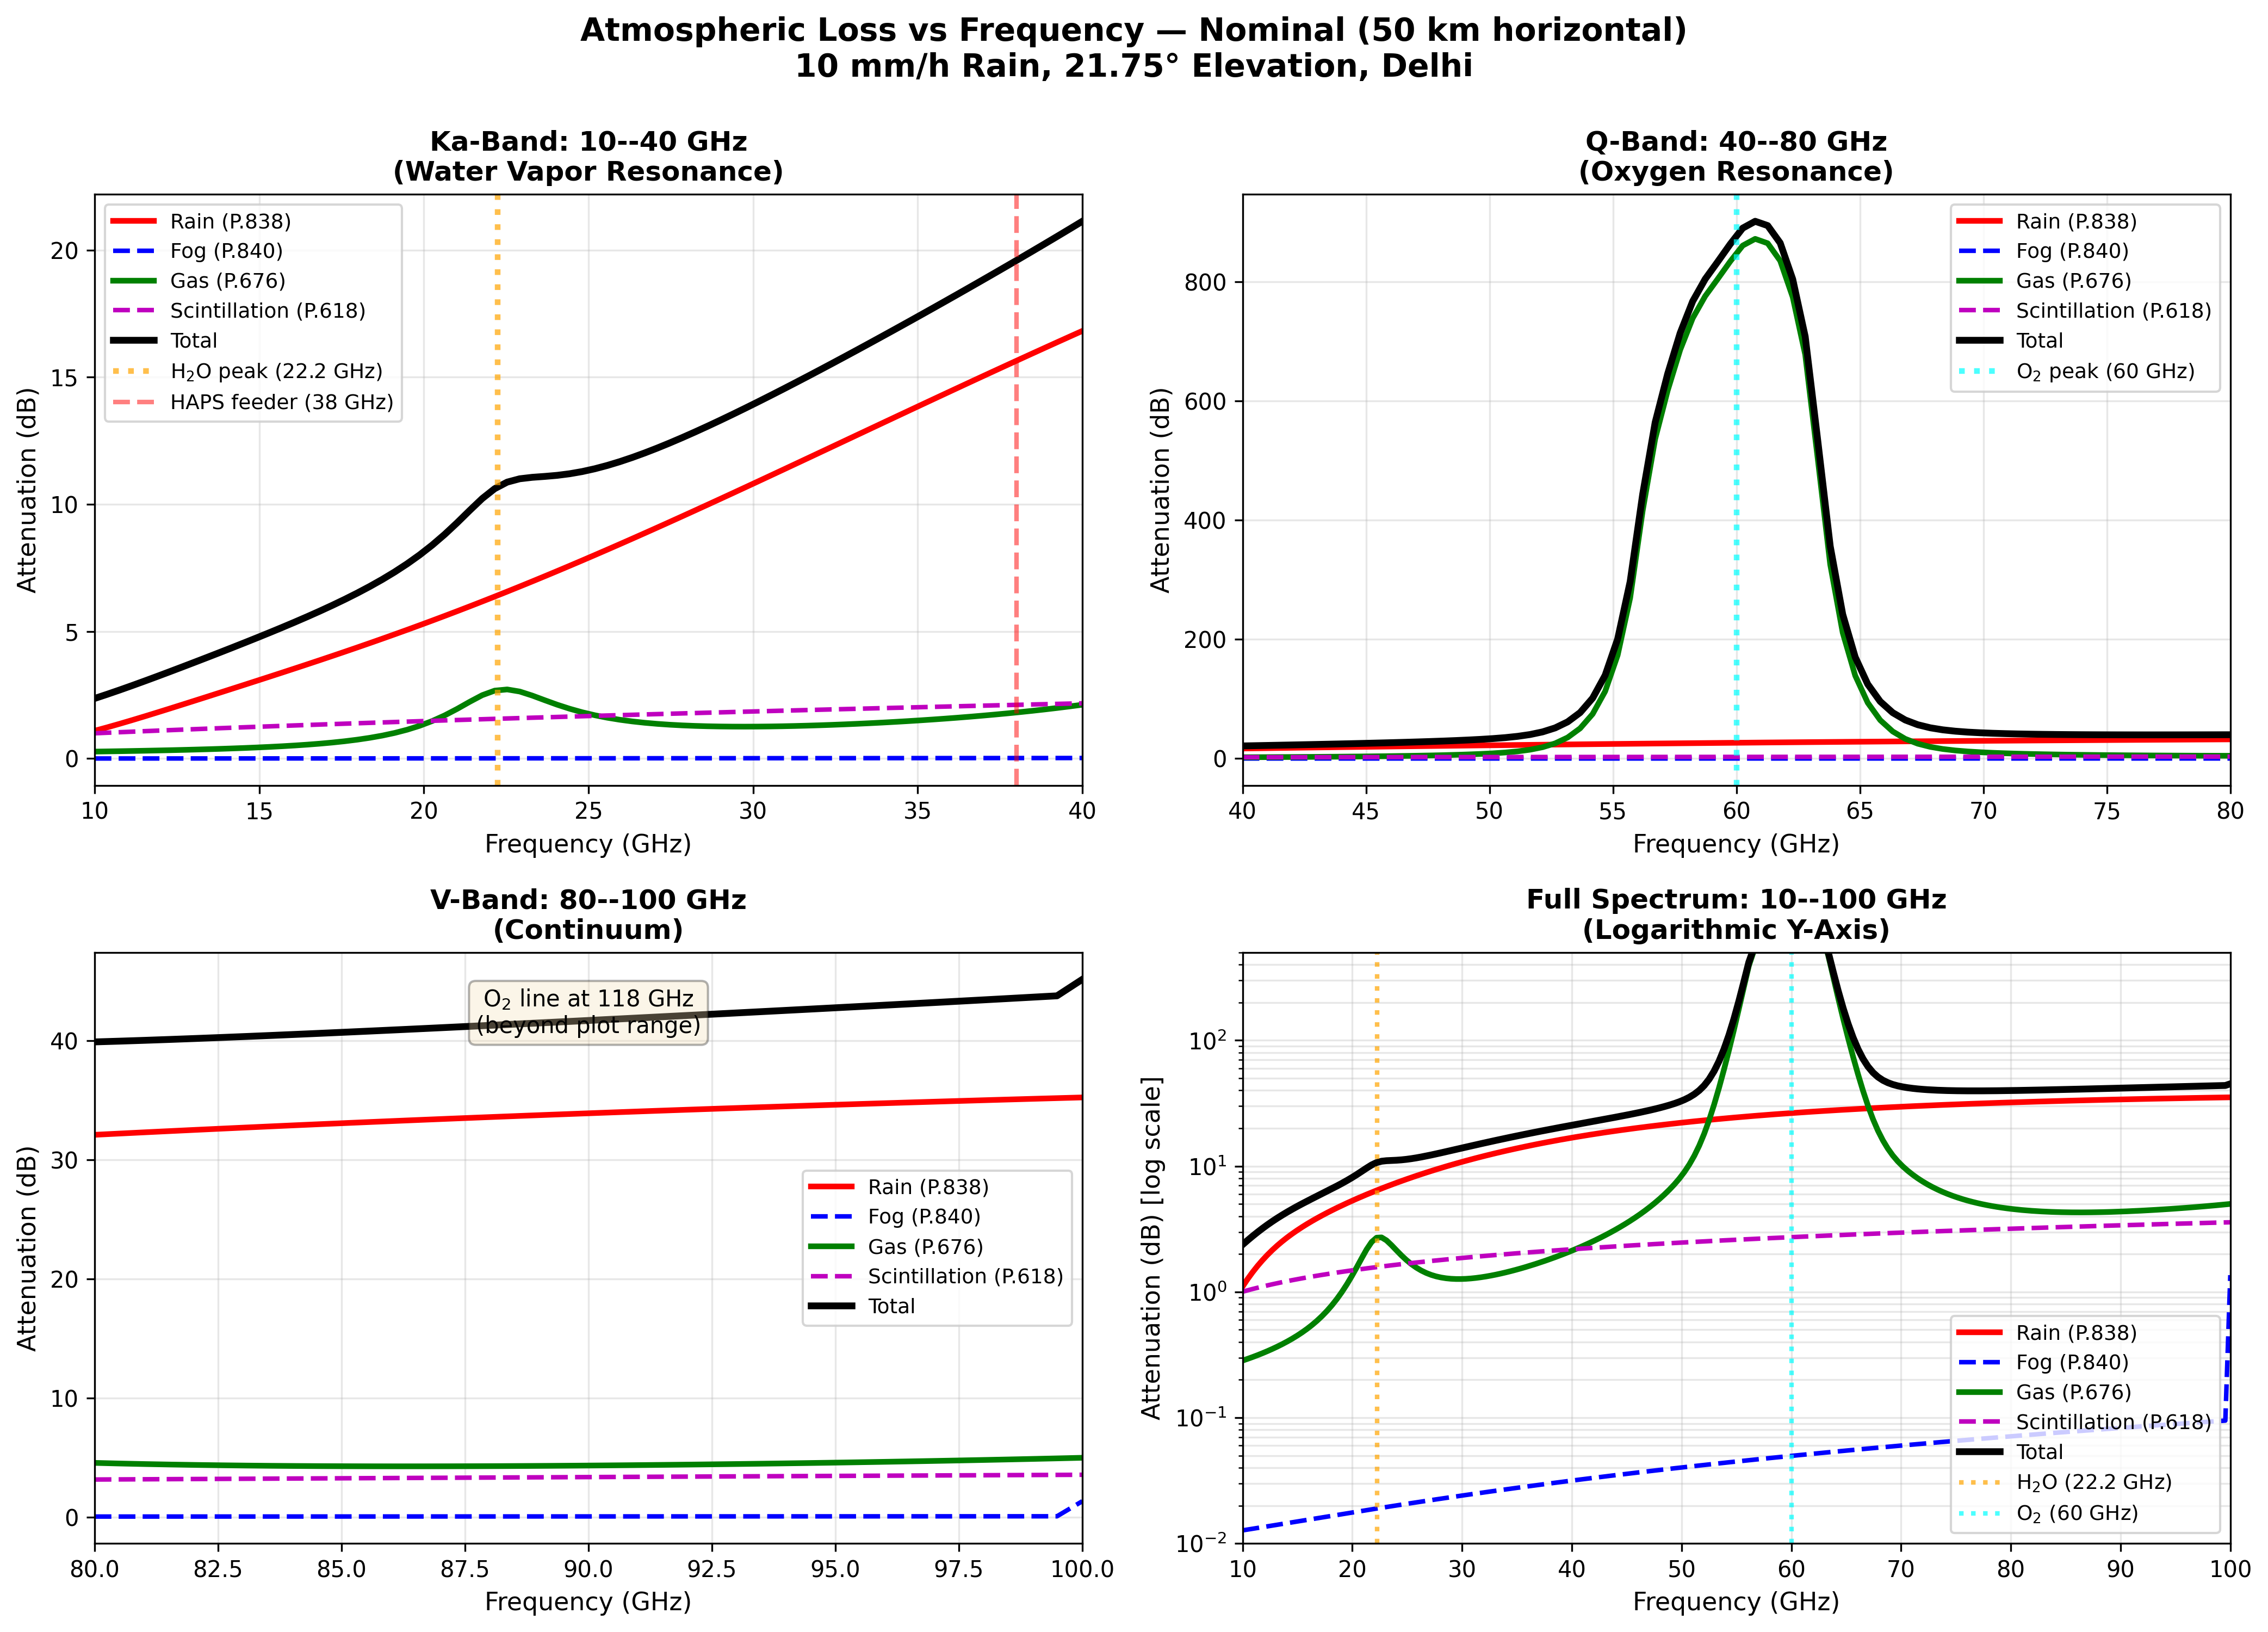
\includegraphics[width=0.95\columnwidth]{./figures/fig_atm_loss_nominal_frequency.png}
\caption{Atmospheric loss vs.\ frequency.}
\label{fig:atm_frequency_nominal}
\end{figure}

\begin{table}[h!]
\centering
\small
\resizebox{\columnwidth}{!}{%
\begin{tabular}{lr}
\hline
\textbf{Component} & \textbf{Loss [dB]} \\
\hline
Rain (P.618/P.838) & 15.65 \\
Fog/cloud (P.840) & 0.02 \\
Atmospheric gas (P.676) & 1.81 \\
Scintillation (P.618, 0.01\% outage) & 4.37 \\
\hline
\textbf{Total} & \textbf{21.85} \\
\hline
\end{tabular}}
\caption{Atmospheric loss breakdown, nominal case: 38\,GHz backhaul link, 21.75$^\circ$ elevation, 54\,km slant path, 10\,mm/h rain, Delhi.}
\label{tab:atm_losses_nominal}
\end{table}

\begin{table}[h!]
\centering
\small
\resizebox{\columnwidth}{!}{%
\begin{tabular}{lr}
\hline
\textbf{Component} & \textbf{Loss [dB]} \\
\hline
Rain (P.618/P.838) & 29.59 \\
Fog/cloud (P.840) & 0.04 \\
Atmospheric gas (P.676) & 3.43 \\
Scintillation (P.618, 0.01\% outage) & 9.53 \\
\hline
\textbf{Total} & \textbf{42.59} \\
\hline
\end{tabular}}
\caption{Atmospheric loss breakdown, worst case: 38\,GHz backhaul link, 11.30$^\circ$ elevation, 102\,km slant path, 10\,mm/h rain, Delhi.}
\label{tab:atm_losses_worstcase}
\end{table}


\textbf{Observation:}
\begin{itemize}
    \item \textbf{Frequency-dependent atmospheric loss:}
    Atmospheric attenuation varies strongly with frequency across the 10--100~GHz range. The spectrum is characterized by distinct molecular absorption resonances rather than a uniform increase in loss with frequency.

    \item \textbf{Water-vapor resonance:}
    A pronounced atmospheric absorption peak occurs near 22.2~GHz due to the water-vapor resonance. This makes the region around 22.235~GHz unsuitable for a low-loss HAPS backhaul/feeder link.

    \item \textbf{Oxygen resonance:}
    A much stronger absorption peak occurs around 60~GHz due to molecular oxygen. The Q-band therefore contains a severe atmospheric-loss region that is undesirable for the backhaul/feeder links.

    \item \textbf{38~GHz backhaul/feeder-band location:}
    The selected 38~GHz HAPS backhaul/feeder frequency lies between the 22.2~GHz water-vapor and 60~GHz oxygen absorption peaks. It therefore avoids the two major molecular-resonance regions and lies in a comparatively lower-loss region of the spectrum.

    \item \textbf{Rain attenuation increases with frequency:}
    Rain attenuation increases with frequency over the considered 10--100~GHz range, as characterized by the frequency-dependent coefficients $k$ and $\alpha$ in ITU-R P.838~\cite{itu_p838}.

    \item \textbf{Frequency-selection tradeoff:}
    Although the 2~GHz service-link frequency would provide lower atmospheric and rain attenuation, it is not directly suitable for the backhaul/feeder links because of regulatory, link-budget, antenna, and capacity constraints. The 38~GHz band therefore represents a practical compromise between propagation loss, available bandwidth, spectrum allocation, and antenna gain.

    \item \textbf{Effect of elevation angle and path length:}
    A lower elevation angle increases the slant-path length and consequently increases the magnitude of the attenuation across the spectrum.

    \item \textbf{Nominal versus worst-case geometry:}
    For the nominal case (50~km horizontal distance and $21.75^\circ$ elevation), the slant path is approximately 54~km, whereas the worst-case case ($11.3^\circ$ elevation and 100~km service-edge distance) has a slant path of approximately 102~km. The longer worst-case path therefore produces substantially higher atmospheric loss while preserving the same frequency-dependent resonance structure.

    \item \textbf{Overall backhaul/feeder-frequency implication:}
    The spectrum analysis indicates that backhaul/feeder-frequency selection cannot be based solely on minimizing frequency-dependent rain attenuation. The selected frequency must simultaneously avoid severe molecular absorption bands and provide adequate spectrum and antenna characteristics. The 38~GHz band satisfies this tradeoff by operating between the major water-vapor and oxygen absorption resonances.
\end{itemize}

The elevation-angle and nominal-vs-worst-case points above are shown directly
in Figure~\ref{fig:rain-vs-distance}, which sweeps rain attenuation
continuously over the HAPS--Gateway horizontal distance rather than at the
two fixed geometries used so far.

\begin{figure}[h!]\centering
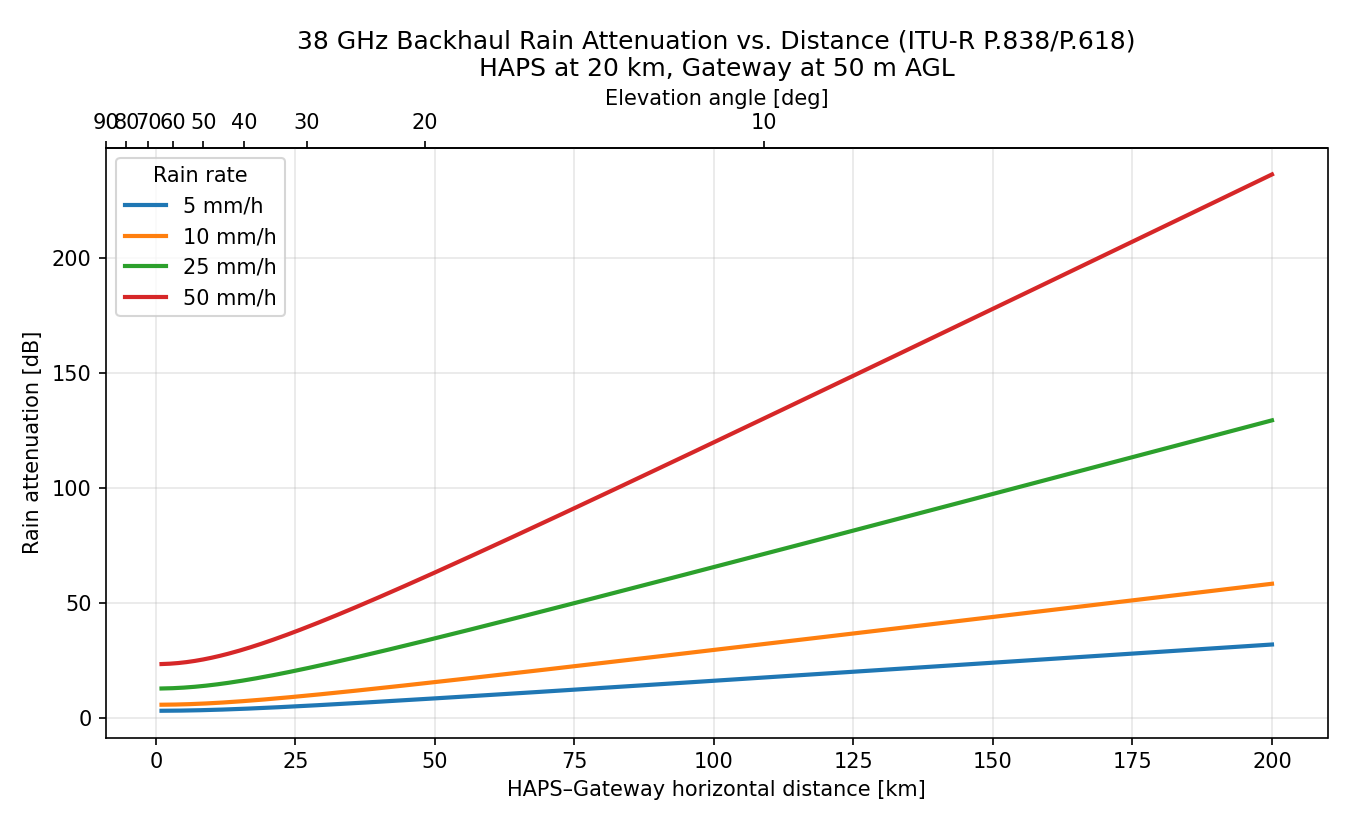
\includegraphics[width=0.95\columnwidth]{./figures/rain_attenuation_vs_distance.png}
\caption{38\,GHz backhaul rain attenuation vs.\ HAPS--Gateway horizontal
distance (ITU-R P.838/P.618), at four fixed rain rates, with the
corresponding elevation angle on the secondary top axis, using the
2\,km effective rain-layer-height convention of
Eq.~\eqref{eq:rain_loss}. At 100\,km ($11.3^\circ$) it gives
$\approx$30\,dB at 10\,mm/h, matching the worst-case backhaul figure
above. (The near-nadir gateway-path result of $\approx$19\,dB uses a
different, site-specific 5.2\,km rain-layer depth and is not directly
comparable to this curve's near-nadir end.) Attenuation grows faster
than linear past $\approx$100\,km as elevation drops and the rain
slant-path lengthens.}
\label{fig:rain-vs-distance}
\end{figure}


\subsection{Loss specific to Multi-HAPS interference}

\label{subsec:multinode-sinr}


The multi-HAPS interference mechanism is fundamentally a spatial phenomenon. A serving HAPS provides the desired signal, while the remaining HAPS transmit on the same radio resource and contribute co-channel interference at the same receiver:

\begin{equation}
\mathrm{HAPS}_0
\rightarrow
\mathrm{Receiver}
\quad\text{(desired)}
\end{equation}

while

\begin{equation}
\mathrm{HAPS}_1,\mathrm{HAPS}_2,\ldots
\rightarrow
\mathrm{same\ receiver}
\quad\text{(interference)}.
\end{equation}

The resulting SINR therefore depends not only on the horizontal distance from the serving HAPS nadir, but also on the angular position of the receiving terminal relative to the interfering HAPS. This dependence is particularly important for the 2~GHz service/relay footprint, where a receiver can lie within the common coverage region of several HAPS.


\subsubsection{General Multi-HAPS SINR Formulation}

The backhaul-link, feeder-link (HAPS-to-UAV), and HAPS-to-UE service-link SINR expressions developed below are each instances of a common HAPS-to-receiver SINR model. For a serving HAPS $h$ and an arbitrary receiving node $r$, the SINR is

\begin{equation}
\boxed{
\begin{aligned}
\gamma_{h,r}=\frac{P_hG_hG_r g_{h,r}}{N_r + \displaystyle\sum_{h'\neq h}P_{h'}G_{h'}G_r g_{h',r}}
\end{aligned}}
\label{eq:general-haps-sinr}
\end{equation}

where $r$ can represent either a Gateway or a UAV.

The numerator represents the desired HAPS transmission, the first term in the denominator represents receiver thermal noise, and the summation represents aggregate co-channel interference from the remaining HAPS.

In the linear domain, the channel gain is obtained from the total propagation loss as

\begin{equation}
g_{h,r}= 10^{-L_{h,r}^{\mathrm{tot}}/10}
\end{equation}

Equivalently, the SINR in decibels is

\begin{equation}
\mathrm{SINR}_{\mathrm{dB}}=10\log_{10}\left(\frac{P_{\mathrm{desired}}}{P_{\mathrm{noise}}+P_{\mathrm{interference}}}\right)
\end{equation}

It is important that the propagation model and the interference model remain conceptually separate. FSPL and atmospheric/scintillation losses determine the channel gain of each desired and interfering link, whereas the SINR equation combines those received powers with receiver noise and co-channel interference.

\subsubsection{HAPS-to-Gateway Backhaul Link}

The backhaul link connects each HAPS to its associated ground gateway and operates at 38~GHz. The desired received signal is generated by the serving HAPS, while transmissions from other HAPS constitute potential co-channel interference if the same time-frequency resource is reused. For a serving HAPS $h$ and gateway $g$, the received desired power is

\begin{equation}
P_{h,g}^{\mathrm{rx}} = P_h G_h G_g g_{h,g}
\end{equation}



where $P\_h$ is the HAPS transmit power, $G\_h$ and $G\_g$ are the transmit and receive antenna gains, respectively, and $g\_{h,g}$ is the channel gain. The baseline propagation loss is modeled using free-space path loss (FSPL):

\begin{equation}
L_{\mathrm{FSPL}}(h,g)=20\log_{10}\left(\frac{4\pi d_{h,g}}{\lambda}\right)
\end{equation}

where $d\_{h,g}$ is the HAPS-to-Gateway slant distance and $\lambda$ is the wavelength.

When atmospheric impairments are included, the total propagation loss is written as

\begin{equation}
L_{h,g}^{\mathrm{tot}}
= L_{\mathrm{FSPL}}
+ A_{\mathrm{rain}}
+ A_{\mathrm{cloud/fog}}
+ A_{\mathrm{gas}}
+ A_{\mathrm{scint}},
\end{equation}

with all terms expressed in dB. The corresponding linear channel gain is

\begin{equation}
g_{h,g} = 10^{-L_{h,g}^{\mathrm{tot}}/10}.
\end{equation}

The backhaul-link SINR is therefore

\begin{equation}
\gamma_{h,g}=\frac{P_h G_h G_g g_{h,g}}{N_g + \displaystyle\sum_{h'\neq h}P_{h'}G_{h'}G_g g_{h',g}},
\label{eq:feeder-sinr}
\end{equation}

where $N\_g$ is the gateway receiver noise power.

The summation term represents potential multi-HAPS interference. It should not be interpreted as necessarily significant for every backhaul-link geometry. In the present constellation, the gateway is located close to the nadir of its serving HAPS, whereas the other HAPS are approximately 65~km away from the serving HAPS. Consequently, their 38~GHz signals experience substantially greater propagation loss than the desired backhaul signal. Under the present power, antenna, and geometry assumptions, this interference is expected to be negligible compared with the receiver noise, resulting in a predominantly noise-limited backhaul link.

Thus, multi-HAPS interference is \emph{modeled as a potential impairment} on the backhaul link, but the present configuration produces a negligible interference contribution. This distinction is important because backhaul-link interference can become relevant in a different frequency-reuse pattern, antenna pattern, gateway placement, or constellation geometry.

\subsubsection{HAPS-to-UAV Relay First Hop (Feeder Link)}

The second HAPS-related link is the feeder link, the first hop of the relay path,

\begin{equation}
\mathrm{HAPS}\rightarrow\mathrm{UAV}\rightarrow\mathrm{UE}.
\end{equation}

For the first hop, the UAV acts as the receiving node. The serving HAPS transmits the desired signal, while the remaining HAPS can simultaneously transmit on the same channel and therefore act as co-channel interferers.

For serving HAPS $h$ and receiving UAV $u$, the desired received power is

\begin{equation}
P_{h,u}^{\mathrm{rx}}= P_hG_hG_u g_{h,u}.
\end{equation}

The corresponding multi-HAPS SINR is

\begin{equation}
\gamma_{h,u}=\frac{P_hG_hG_u g_{h,u}}{N_u + \displaystyle\sum_{h'\neq h}P_{h'}G_{h'}G_u g_{h',u}},
\label{eq:haps-uav-sinr}
\end{equation}

where $N\_u$ is the thermal noise power at the UAV receiver.

This is the primary multi-HAPS interference scenario considered in the relay architecture. The interference term explicitly represents simultaneous transmissions from the non-serving HAPS to the same UAV receiver.

The channel gain for every HAPS-to-UAV path is obtained from its corresponding propagation loss:

\begin{equation}
g_{h,u}= 10^{-L_{h,u}^{\mathrm{tot}}/10}.
\end{equation}

The total loss may be represented as

\begin{equation}
L_{h,u}^{\mathrm{tot}}=L_{\mathrm{FSPL}}(h,u)+ A_{\mathrm{atm}}(h,u)+ A_{\mathrm{scint}}(h,u),
\end{equation}

where $A\_{\mathrm{atm}}$ represents the relevant atmospheric attenuation components and $A\_{\mathrm{scint}}$ represents tropospheric scintillation when included in the channel realization.

Unlike the low-altitude UAV-to-UE link, the HAPS-to-UAV path is a high-altitude slant path and is therefore dominated by the geometry between the stratospheric HAPS and the receiving UAV. The same propagation model must be applied independently to the desired HAPS and each interfering HAPS so that their different slant ranges and elevation angles are reflected in the resulting SINR.

\subsubsection{UAV-to-UE Relay Second Hop}

The second relay hop is

\begin{equation}
\mathrm{UAV}\rightarrow\mathrm{UE}.
\end{equation}

This link is not itself a multi-HAPS interference link because the transmitter is the UAV rather than the HAPS. Its SINR should therefore be modeled using the relevant UAV transmitters and receivers:

\begin{equation}
\gamma_{u,k}=\frac{P_uG_uG_k g_{u,k}}{N_k + \displaystyle\sum_{u'\neq u}P_{u'}G_{u'}G_k g_{u',k}},
\label{eq:uav-ue-sinr}
\end{equation}

where $k$ denotes the UE and $u'$ denotes other simultaneously transmitting UAVs.

If only one UAV is transmitting in the considered resource block, the interference summation is zero and the link becomes noise-limited. If multiple UAVs reuse the same channel, their transmissions constitute the interference term.

\subsection{Relay Path Analysis (HAPS\texorpdfstring{$\rightarrow$}{->}UAV\texorpdfstring{$\rightarrow$}{->}UE)}
\label{sec:relay-path-analysis}

The two SINR expressions above (Eq.~\eqref{eq:haps-uav-sinr}, \eqref{eq:uav-ue-sinr})
define the relay link; this section evaluates them numerically as a
decode-and-forward (DF) two-hop path, implemented in
\texttt{uav\_relay\_two\_hop\_capacity\_bps\_hz()}. The first hop (the feeder link) reuses the
38\,GHz backhaul-link slant-path model (\S III.B; UAV hovering at 500\,m, ITU-P.618
scintillation included) since both the backhaul link and this hop are high-altitude,
high-frequency, 38\,GHz links; the second hop reuses the 2\,GHz
landscape-dependent LoS/NLoS blended model (\S III.C) since the UAV, like
the HAPS, is a low-altitude access node subject to building blockage. The
two hops are combined DF, so the end-to-end capacity is the bottleneck of
the two:
\begin{equation}
C_{\text{uav-relay}} = \min\!\left(C_{\text{haps-uav}},\, C_{\text{uav-ue}}\right).
\label{eq:uav-relay-capacity}
\end{equation}

\noindent\textbf{Minimum design SINR.} A link is only useful if it clears a
minimum design SINR set by the target block-error rate (BLER) of the
modulation and coding scheme (MCS) it needs to run, plus an implementation
margin:
\begin{equation}
\gamma_{\text{min,design}} = \mathrm{SINR}_{\text{MCS}}(\text{target BLER}) + \text{margin}.
\label{eq:sinr-min-design}
\end{equation}
For the direct HAP\,$\rightarrow$\,vehicle-UE service link, a lower bound of
$\gamma_{\text{SINR}}=-5$\,dB is used as the minimum link quality for a UE to
be considered active and able to receive signals from the HAP -- close to
the $\approx-6$\,dB required by the lowest-order 3GPP NR MCS (QPSK, CQI
index~1, $\mathrm{BLER}=10\%$)~\cite{3gpp_ts38214}. The 38\,GHz feeder hop
is held to a higher design floor: relaying is only worth its extra hop and
extra hardware if it can run at least a moderate-order MCS (16-QAM,
$\mathrm{CQI}\approx7$, $\mathrm{SINR}_{\text{MCS}}\approx+5$\,dB at 10\%
BLER~\cite{3gpp_ts38214}), so with a 3\,dB implementation margin this
document targets
$\gamma_{\text{min,design}}^{\text{haps-uav}}\approx+8$\,dB for the
HAPS\,$\rightarrow$\,UAV hop.

The relay path is swept over the HAPS\textendash UAV horizontal distance
0--100\,km across all four landscapes, and Figure~\ref{fig:uav-relay-comparison}
plots the resulting SINR on each hop against the direct HAPS\,$\rightarrow$\,UE link.

\begin{figure}[t]
\centering
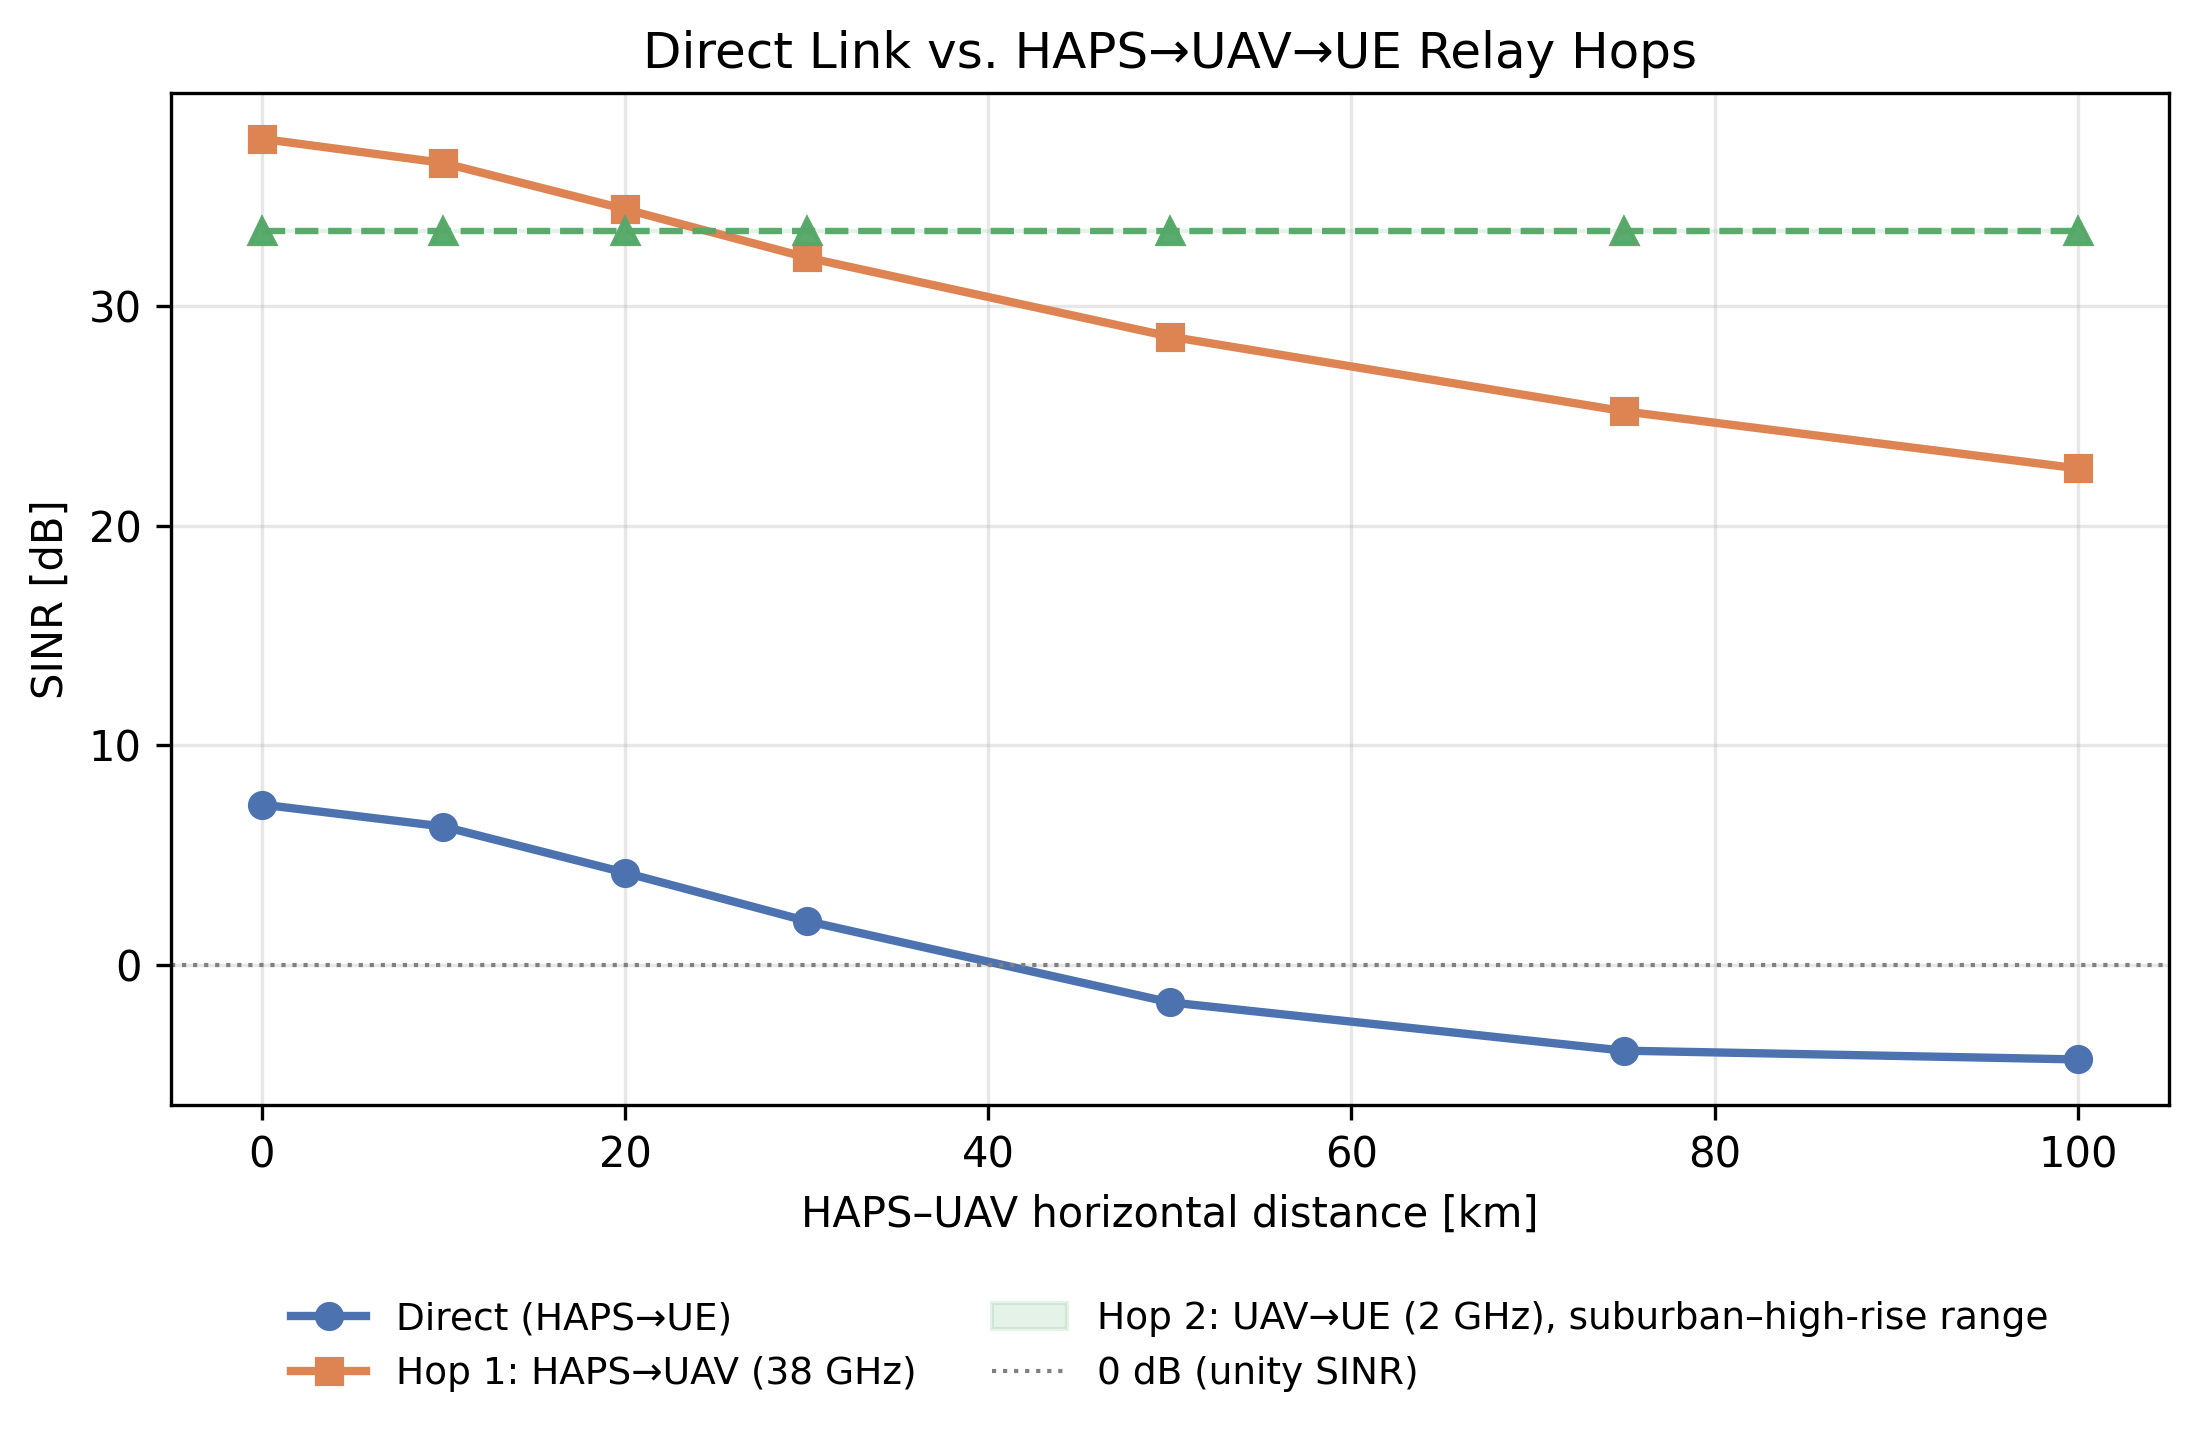
\includegraphics[width=\linewidth]{./figures/12_uav_relay_comparison.png}
\caption{Direct HAPS\,$\rightarrow$\,UE SINR (suburban, averaged in dB over 24 azimuths, including co-channel interference from the other two HAPS) vs.\ the two UAV relay hops, as a function of HAPS\textendash UAV horizontal distance. The HAPS\,$\rightarrow$\,UAV feeder hop (orange, including interference from the other HAPS, which is about 35\,dB below the noise floor) starts at $+37.6$\,dB at nadir and stays above $+22$\,dB at 100\,km, well above the $+8$\,dB design floor (Eq.~\eqref{eq:sinr-min-design}). The UAV\,$\rightarrow$\,UE access hop (green, suburban and high-rise identical at 500\,m) is $+33.4$\,dB. The direct link falls from $+7.3$\,dB at nadir to $-9.1$\,dB at 100\,km.}
\label{fig:uav-relay-comparison}
\end{figure}

\noindent\textbf{The relay outperforms the direct link at every distance,
because co-channel interference from the other HAPS limits the direct service link.}
The UAV hovers directly above the user it serves (\S II), so its horizontal distance
from the user is small and fixed, while its distance from the serving HAPS grows with
the user's own distance from the HAPS nadir. The UAV\,$\rightarrow$\,UE hop therefore stays
at $\mathrm{SINR}\approx+33$\,dB regardless of where the UAV is deployed.
The HAPS\,$\rightarrow$\,UAV hop is a 38\,GHz
slant path with antenna gains $G_h=13.8$\,dBi (HAPS side) and $G_u=30.7$\,dBi (UAV side),
matching a published 30\,GHz HAPS backhaul-class budget and a UAV-mountable mmWave
patch-array antenna~\cite{karaman2025haps,anim2021uav}. Its SINR is $+37.6$\,dB at nadir and
falls to $+22.6$\,dB at 100\,km as the elevation angle drops to $11^\circ$. Its interference
term is about 35\,dB below the noise floor, so the hop is noise-limited. The direct
HAPS\,$\rightarrow$\,UE link is different: it shares the 2\,GHz band with the other two HAPS, and its
SINR falls from $+7.3$\,dB at nadir to $-9.1$\,dB at 100\,km. Its capacity therefore drops from
$2.7$ to $0.2$\,bits/s/Hz. The relay's end-to-end capacity is $C_{\text{uav-relay}} = \min(C_{\text{haps-uav}}, C_{\text{uav-ue}})$:
$11.1$\,bits/s/Hz at nadir, where the UAV\,$\rightarrow$\,UE access hop is the bottleneck, and $7.5$\,bits/s/Hz at 100\,km,
where the feeder hop is the bottleneck (from about 30\,km outward). This result depends on two
modelling choices: the 38\,GHz scintillation fade from the ITU-R P.618 table
(about 0.2\,dB at zenith), and the ITU-R F.699 sidelobe envelope used for the interferers and the
receive patterns (Section~III, interference model). The DQN association agent (\S\ref{sec:lstm-dqn-motivation}) can route traffic through the UAV relay, as one of its six actions.

\subsubsection{HAPS-to-UE Service Link}

The multi-HAPS service link is

\begin{equation}
\mathrm{HAPS}\rightarrow\mathrm{UE}.
\end{equation}

Consider a three-HAPS equilateral constellation with serving HAPS $S$ at the origin and interfering HAPS $I_1$ and $I_2$ separated from $S$ by approximately 65~km. Let a receiver be located at horizontal distance $r$ from the serving-HAPS nadir and at azimuth angle $\theta$. The horizontal position of the receiver may be written as

\begin{equation}
\mathbf{x}_r = \begin{bmatrix} r\cos\theta\\r\sin\theta\end{bmatrix}.
\end{equation}

For an interfering HAPS $i$ located at azimuth $\theta_i$ and horizontal separation $D$ from the serving HAPS, the corresponding slant range is

\begin{equation}
d_i(r,\theta)
=
\sqrt{
 h_i^2
 + r^2
 + D^2
 -2rD\cos(\theta-\theta_i)
},
\label{eq:interferer-slant-range}
\end{equation}

where $h_i$ represents the effective vertical separation between HAPS $i$ and the receiver. The desired slant range is

\begin{equation}
d_s(r)
=
\sqrt{h_s^2+r^2}.
\label{eq:desired-slant-range}
\end{equation}

Thus, even when two receivers have the same radial distance $r$, their desired and interfering received powers can be different because their angular positions relative to $I_1$ and $I_2$ are different.

The angular separation between the desired-HAPS direction and an interfering-HAPS direction, as viewed from the receiver, is the angle subtended by the two HAPS at the receiver. It can be defined from the corresponding line-of-sight vectors as

\begin{equation}
\Delta\phi_i
=
\cos^{-1}
\left(
\frac{
(\mathbf{p}_s-\mathbf{x}_r)\cdot(\mathbf{p}_i-\mathbf{x}_r)
}{
\left\|\mathbf{p}_s-\mathbf{x}_r\right\|
\left\|\mathbf{p}_i-\mathbf{x}_r\right\|
}
\right),
\label{eq:angular-subtend}
\end{equation}

where $\mathbf{p}_s$ and $\mathbf{p}_i$ denote the three-dimensional positions of the serving and interfering HAPS, respectively. Thus, $\Delta\phi_i$ is the actual angular separation between the desired and interfering directions at the receiver. In the present free-space propagation model, this angle does not by itself produce constructive or destructive combining; rather, the receiver position changes the corresponding slant ranges and hence the desired and interfering received powers. If directional receive or transmit beam patterns are introduced, the same angular separation can additionally affect the antenna gains toward the serving and interfering HAPS.

The multi-HAPS SINR can therefore be viewed as a spatial function

\begin{equation}
\gamma(r,\theta)
=
\frac{
P_sG_sG_r g_s(r)
}{
N_r
+
\displaystyle\sum_{i\in\mathcal{I}}
P_iG_iG_r g_i(r,\theta)
},
\label{eq:spatial-sinr}
\end{equation}

where $\mathcal{I}$ denotes the set of interfering HAPS. Because $g_i(r,\theta)$ changes with the receiver position, the SINR forms a spatial map rather than a function of distance alone.

\paragraph{Good and bad reception regions.}

The original service-link results demonstrate this spatial behavior directly. At a horizontal distance of $r=50$~km, the SINR varies from approximately $-7.40$~dB when the receiver is oriented toward interferer $I_1$ ($\theta=0^\circ$) to approximately $+2.54$~dB when positioned away from the constellation ($\theta=210^\circ$), giving a spatial spread of approximately 9.94~dB. The corresponding constellation-sector representation identifies a good sector approximately in the $120^\circ$--$290^\circ$ region, away from the interfering HAPS, and a bad sector approximately in the $330^\circ$--$75^\circ$ region, toward the interferers.

These regions should be interpreted as regions of higher and lower SINR, respectively. In the good sector, the interfering HAPS contribute less received power relative to the serving HAPS, reducing the interference term. In the bad sector, one or more interfering HAPS have a more favorable geometry to the receiver, increasing their received interference power and reducing the SINR. Hence, multi-HAPS interference produces a spatially non-uniform service area even when the receiver is at the same radial distance from the serving HAPS.

This observation is also reflected in the min--max angular spread of the SINR results. The angular variation becomes increasingly important with distance, so a distance-only link budget is insufficient to characterize the interference environment. The receiving-terminal position relative to the constellation must be retained explicitly in the multi-HAPS model.

Figure~\ref{fig:app-constellation-sectors} shows this constellation geometry directly, together with
the resulting spatial SINR pattern it produces at r~=~50\,km: a good sector (away from both
interferers) and a bad sector (toward them), rather than a distance-only falloff.

\begin{figure}[h!]\centering
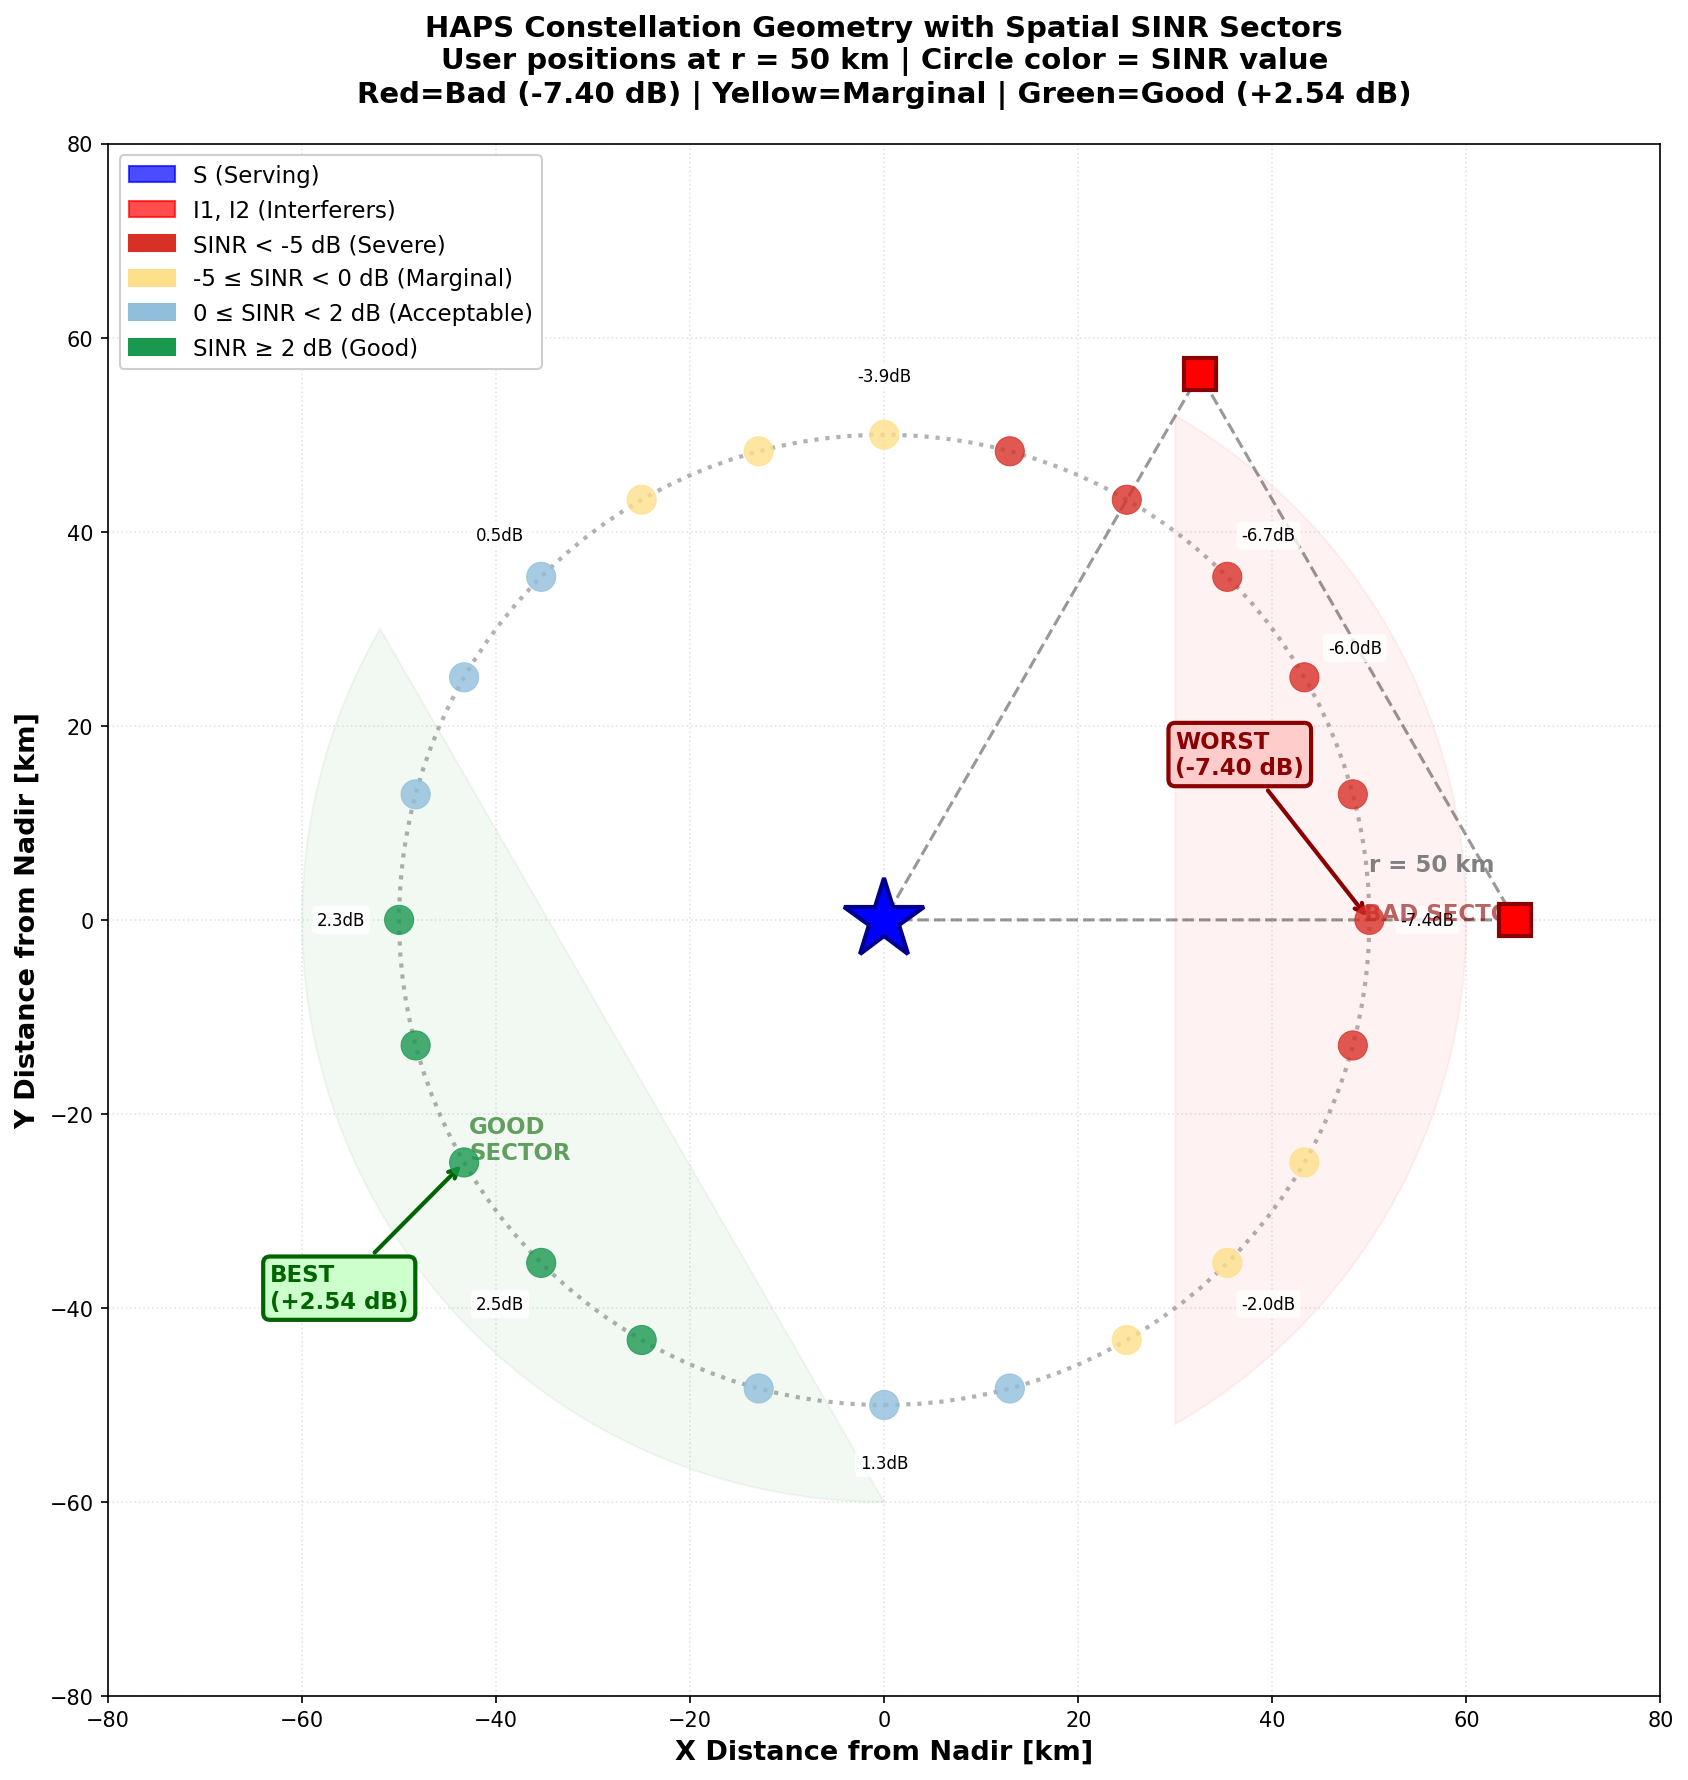
\includegraphics[width=0.85\columnwidth]{./figures/constellation_with_sectors.png}
\caption{HAPS constellation geometry (true 65\,km equilateral triangle: S at origin, I1 at $0^\circ$, I2 at $60^\circ$) with spatial SINR sectors at r~=~50\,km. Good sector (green, away from interferers, $\sim$120--290$^\circ$) vs.\ bad sector (red, toward interferers, $\sim$330--75$^\circ$). Best +2.54\,dB @ $210^\circ$; worst --7.40\,dB @ $0^\circ$.}
\label{fig:app-constellation-sectors}
\end{figure}

\subsubsection{Multi-HAPS Interference Conclusion}

Good/bad sector result: At $r = 50$~km, SINR ranges from
$-7.40$~dB toward interferer $I_1$ ($\theta = 0^\circ$) to
$+2.54$~dB away from the constellation ($\theta = 210^\circ$),
a $9.94$~dB spread. This maps to a good sector
(approximately $120^\circ$--$290^\circ$, away from interferers) and
a bad sector (approximately $330^\circ$--$75^\circ$, toward them),
as shown in Figure~\ref{fig:app-constellation-sectors}.

So multi-HAPS interference makes the service area spatially non-uniform even at fixed radial distance $r$.

The same interference term exists in the general SINR formula for the 38 GHz backhaul link, but under the current geometry (gateway near serving-HAPS nadir, interferers ~65 km away) that interference is expected to be negligible vs. receiver noise.
Bottom line: the service-link analysis is scoped to the angularly-varying interference pattern (good/bad sectors, SINR spread), while the backhaul link is reported as predominantly noise-limited under this constellation/gateway placement.



\paragraph{Multihaps validation from simulation}

Figure~\ref{fig:multinode-interference} quantifies the interference-induced SINR penalty across the 100~km service footprint, averaged over all 24 angular positions around the constellation (all four landscapes are numerically identical at this tier, so a single line is shown rather than four overlapping ones). The shaded band is the min--max spread from that angular variation, not measurement uncertainty. Mean SINR falls from $+6.3$\,dB at 10\,km to $-4.3$\,dB at 100\,km, while the band widens from 1.95\,dB at 10\,km to 11.94\,dB at 75\,km -- beyond $\sim$30\,km, angular position relative to the 65\,km equilateral constellation dominates over distance decay alone. In the received-power trace, the downward bend after $\sim$60\,km marks the transition from an interference-limited to a path-loss-dominated regime: desired power falls faster than interference, so the absolute signal level keeps decaying even once interference stops being the dominant cause of degradation. The network must therefore employ TDMA, FDMA, beamforming, or power control to manage this interference and its spatial variability.

\begin{figure}[h!]\centering
\begin{subfigure}[b]{0.49\columnwidth}\centering
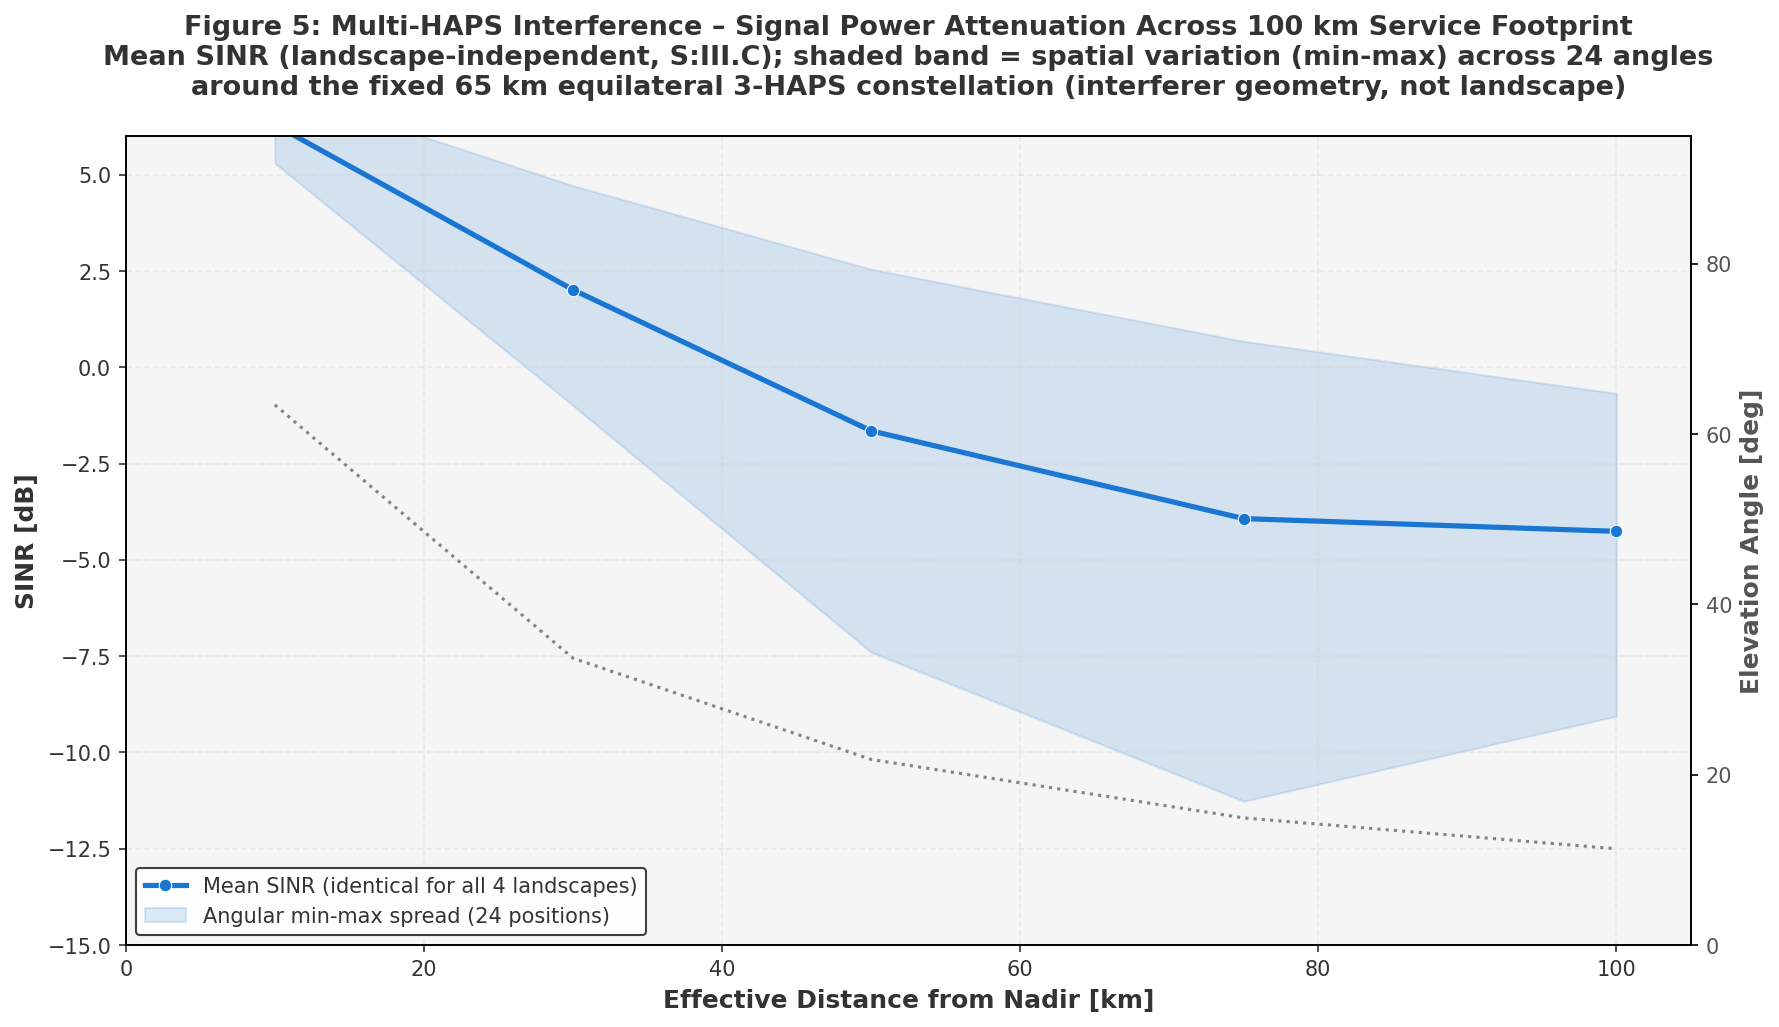
\includegraphics[width=\linewidth]{./figures/figure5_multi_haps_sinr_mean.png}
\caption{Mean SINR and angular min--max spread across 100\,km service footprint.}
\end{subfigure}\hfill
\begin{subfigure}[b]{0.49\columnwidth}\centering
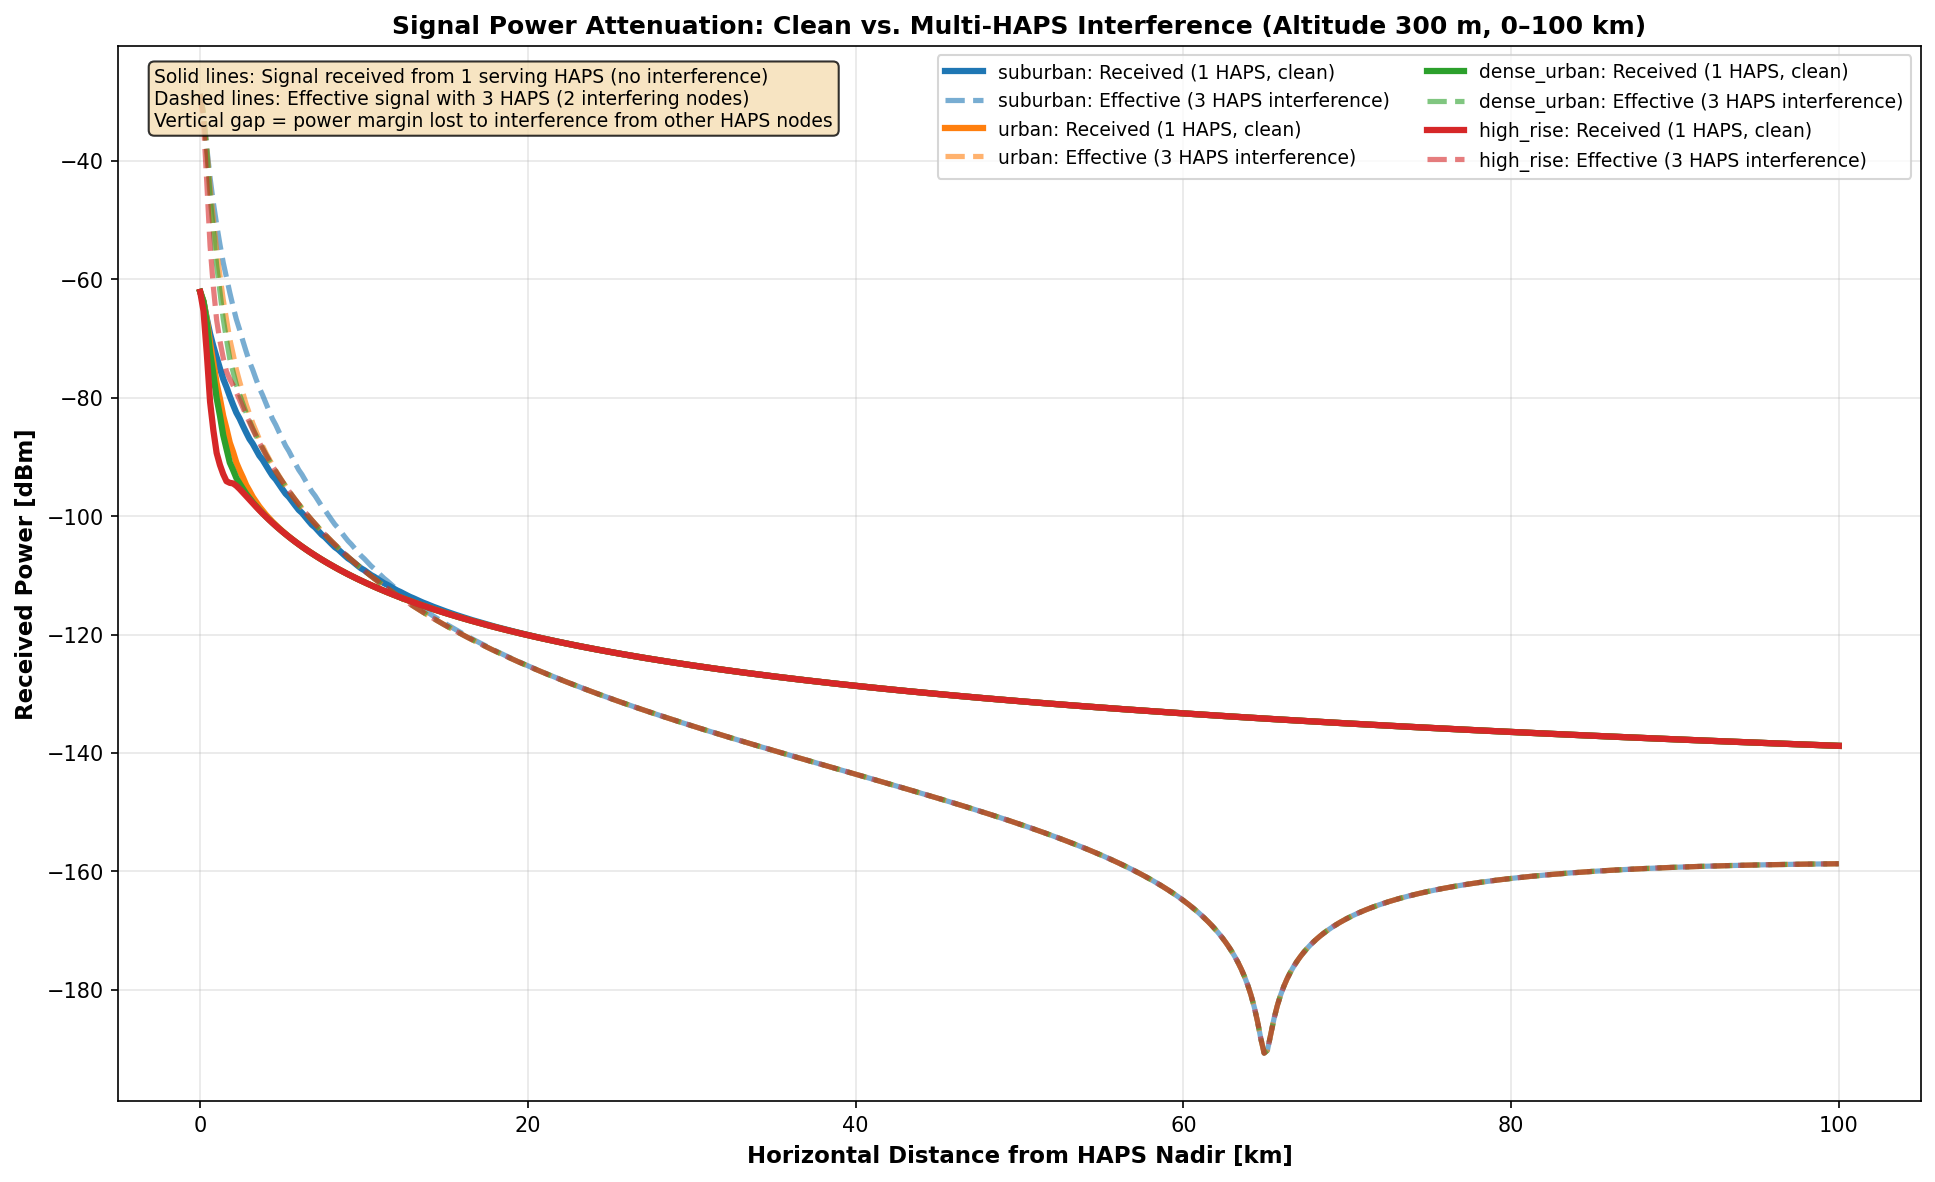
\includegraphics[width=\linewidth]{./figures/figure5_model_received_power.png}
\caption{Received-power comparison showing clean vs. effective power under three-HAPS interference.}
\end{subfigure}
\caption{Multi-HAPS interference characterization at the service link: (a) SINR variability and (b) received-power degradation.}
\label{fig:multinode-interference}
\end{figure}

Figure~\ref{fig:sinr-service-link} decomposes this along one representative direction into SINR\_Single (no interference), SINR\_Actual (with 3-node interference), and SINR\_Interferers (interference-to-noise ratio), computed from Equation~\eqref{eq:spatial-sinr} using pure free-space path loss. SINR\_Interferers stays positive (0.95--4.6\,dB) across the full 10--100\,km range, so the link never leaves the interference-limited regime; SINR\_Actual itself only turns negative between 30\,km ($+2.0$\,dB) and 50\,km ($-1.6$\,dB), reaching $-4.3$\,dB at 100\,km -- because path loss to the serving HAPS eventually dominates the link budget, not because the interference term grows.

\begin{figure}[h!]\centering
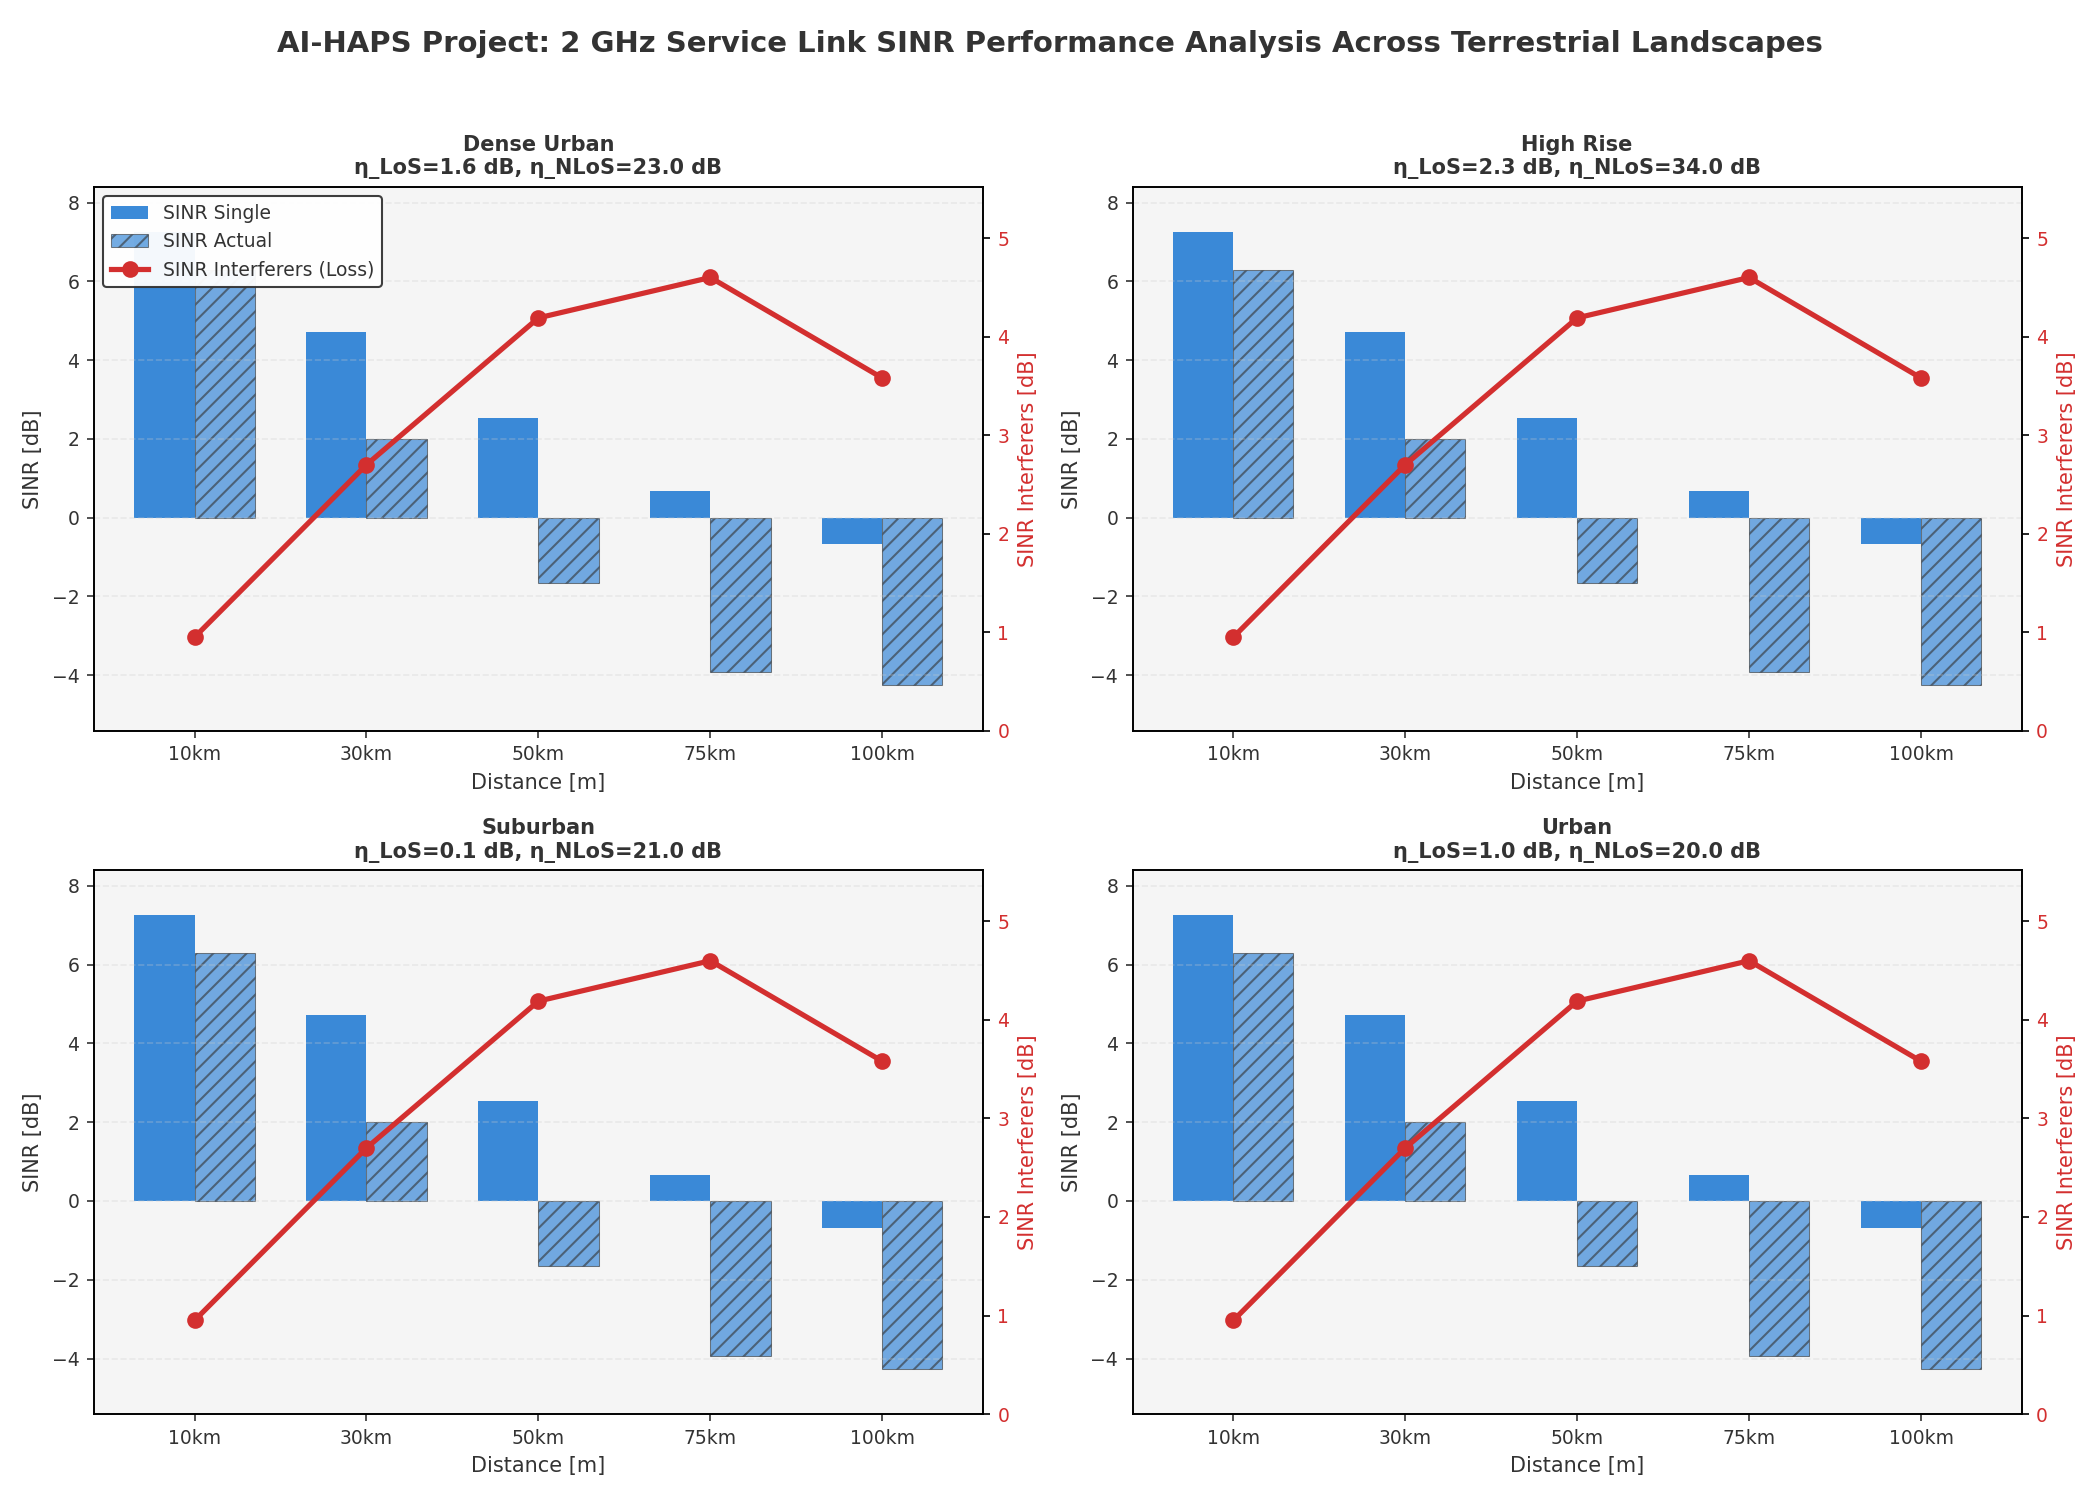
\includegraphics[width=0.95\columnwidth]{./figures/haps_sinr_trellis.png}
\caption{2~GHz service link SINR, four identical landscape subplots (identical across landscapes, \S III.C), 10--100\,km distances.}
\label{fig:sinr-service-link}
\end{figure}

Figure~\ref{fig:sinr-feeder-link} shows the 38~GHz backhaul-link SINR for gateway offsets of 10--500~m from nadir (gateway at 50\,m altitude, HAPS at nominal stratospheric altitude), including the HAPS-side and Gateway-side antenna gains of \S\ref{subsec:backhaul-geometry} ($G_h=13.8$\,dBi, $G_g=39.7$\,dBi). The backhaul slant range is set by the HAPS altitude ($\sim$20\,km), against which a 10--500\,m horizontal offset is negligible, so SINR is essentially flat at $\approx+38.0$--$38.1$\,dB across this range -- strongly positive once the directional antenna gains are included, versus the deeply negative result obtained when the link budget used raw transmit power alone (\S\ref{subsec:backhaul-geometry}). The interfering HAPS, by contrast, sit at a slant range of $\sim$65--68\,km (equilateral-triangle geometry, \S III.A); the resulting interference power is $\approx-35$\,dB below the noise floor. This assumes that each interferer's main beam points at its own service area, so the gateway sees it through the sidelobe envelope of ITU-R F.699 (floored at $-10$\,dBi), and that the gateway dish is off-boresight by about $73^\circ$ toward the interferer, so its gain there is also the $-10$\,dBi floor. The backhaul link is therefore \textbf{noise-limited, not interference-limited}, unlike the service link.

\begin{figure}[h!]\centering
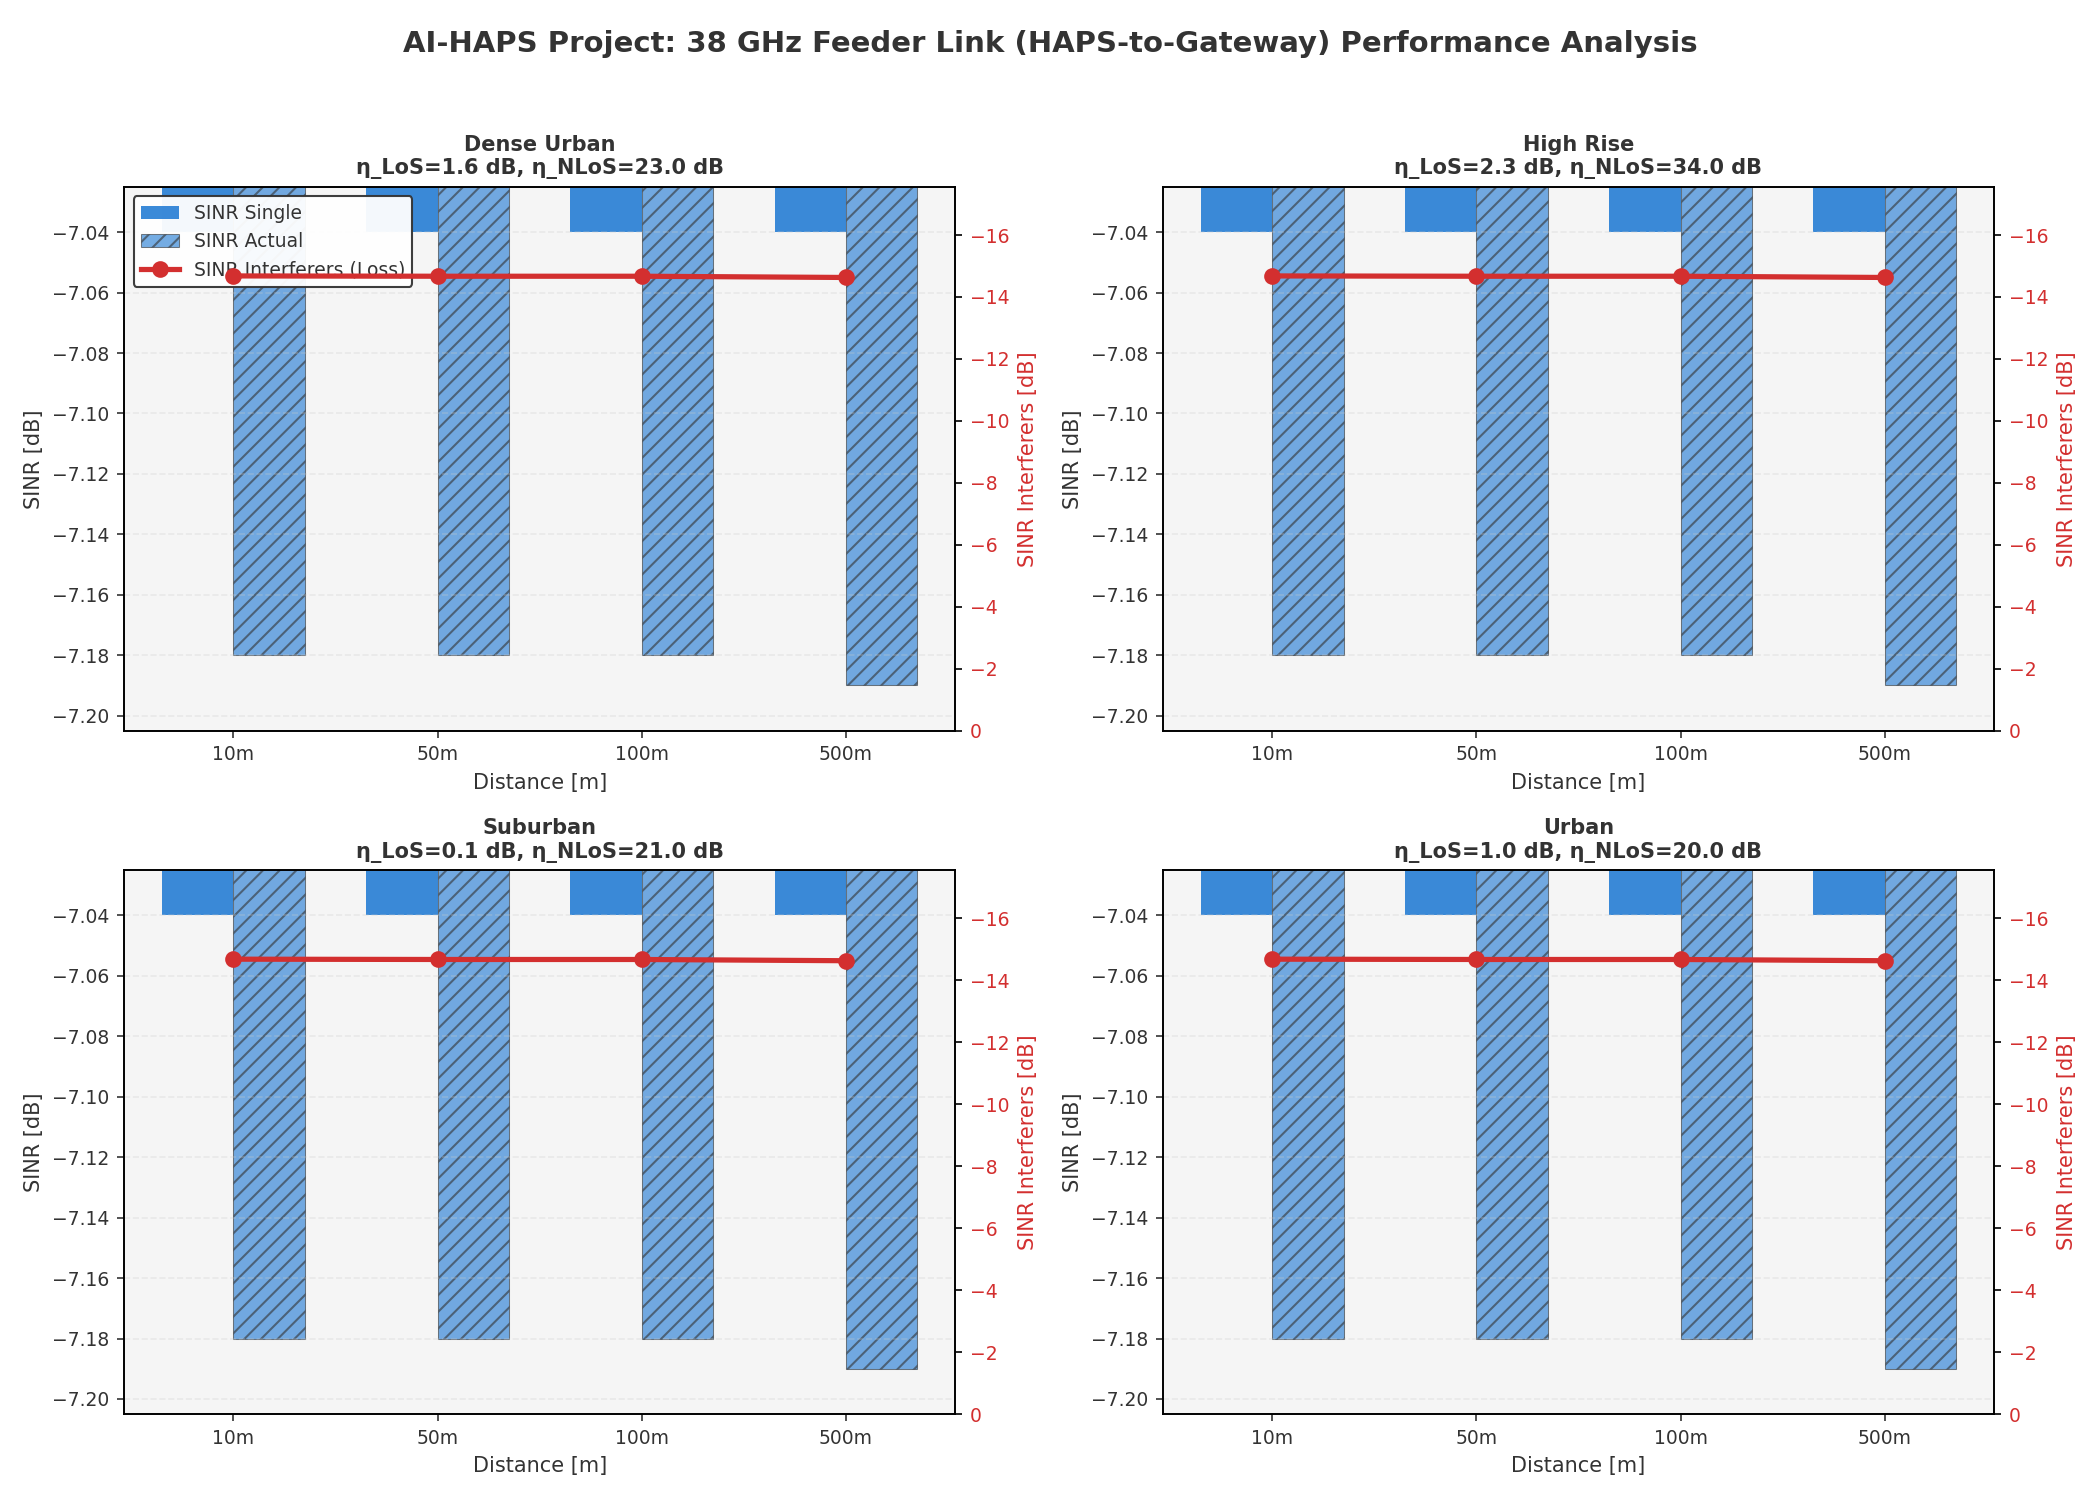
\includegraphics[width=0.95\columnwidth]{./figures/haps_feeder_link_38ghz.png}
\caption{38~GHz backhaul link (HAPS-to-Gateway) SINR, four identical landscape subplots (identical across landscapes, \S III.C), 10--500\,m distances.}
\label{fig:sinr-feeder-link}
\end{figure}

\subsubsection{Service Link (2~GHz): SINR Effects from Distance and Constellation Geometry}

In summary, 2~GHz service-link SINR is governed by horizontal distance $r$ from the HAPS nadir and by the receiver's angular position relative to the two interfering HAPS in the 65~km equilateral-triangle constellation (\S\ref{subsec:multinode-sinr}, Figure~\ref{fig:app-constellation-sectors}); the landscape environment has no effect, since both the desired and interfering links use free-space path loss. Distance alone is therefore insufficient to characterize interference conditions, motivating the DRL-based adaptive scheduling approach that follows.

\subsection{DRL Comparison with Per-User State}
\label{sec:assoc-baseline-setup}

Building on the 3-HAPS constellation (Table~\ref{tab:config}) and the SINR model of
Sections~III.A--III.C, this section defines the per-user HAPS-association task used
to compare rule-based and learned (DRL) policies: at each simulated hour, every one
of $N=50$ users must choose which of the 3 HAPS to associate with, based on a
per-user state consisting of its SINR to each of the 3 HAPS
(dB, Eq.~\eqref{eq:sinr}), its horizontal distance to each (km), each HAPS's battery
state of charge (\%), and the current weather (rain rate, visibility, hour of day).
One episode is one simulated day (24 hourly steps). Per episode, user positions and
each HAPS's initial battery SoC ($\mathcal{U}(30,100)\,\%$) are drawn once and held
fixed; weather is drawn once per episode (\texttt{WeatherScenarioGenerator},
\texttt{random\_mix} mode). Each HAPS's battery is charged by a fixed diurnal solar
profile and discharged by a constant platform and backhaul draw. The per-user load is not modelled, so the association
policy does not change the battery state; time of day is the only driver of SoC. Rain de-rates only the
backhaul-link throughput credit (Section~\ref{subsec:multinode-sinr}), not the 2~GHz
service SINR.

Three rule-based (non-learned) association policies are evaluated:
\begin{itemize}\setlength{\itemsep}{0pt}
  \item \textbf{Random}: uniform-random platform choice each hour (sanity floor).
  \item \textbf{Max-SINR}: each user $k$ always associates to the platform
    \begin{equation}
    p^\star = \operatorname*{arg\,max}_{p} \; \mathrm{SINR}_{k,p},
    \end{equation}
    each user is connected to one platform at a time, chosen from the three direct links; the other two links are not used. No memory of battery or fairness state, no learning.
  \item \textbf{Max-throughput}: each user takes the option with the highest throughput across all six options (direct and UAV-relay for each HAPS), at each hour; no memory, no learning. It assumes perfect, instantaneous knowledge of every option's SINR and capacity, which a deployed system cannot have, so it is a theoretical upper bound on single-hour throughput rather than a deployable policy.
\end{itemize}
All three are evaluated over 50 held-out episodes (random seed 999) using Jain's fairness index,
outage fraction (SINR below $-2$~dB, the severe-outage threshold measured in
Table A.3), and aggregate throughput (Shannon capacity, summed over
users) as metrics. Jain's fairness index measures how evenly a resource (here,
per-user throughput $T_k$) is shared across the $N$ users,
\begin{equation}
J(\mathbf{T}) = \frac{\left(\sum_{k=1}^{N} T_k\right)^2}{N \sum_{k=1}^{N} T_k^2},
\qquad J \in \left(\tfrac{1}{N},\,1\right],
\end{equation}
with $J=1$ when all users receive identical throughput (perfectly fair) and $J\to 1/N$
when the resource is concentrated on a single user (maximally unfair); it is reported
alongside outage and aggregate throughput because a policy that maximizes total
throughput can still do so unfairly, e.g.\ by starving low-SINR users.

\paragraph{Throughput.} The per-user throughput is the Shannon capacity of the chosen link, in bits/s/Hz: $T_k=\log_2(1+\gamma_k)$ for a direct link, where $\gamma_k$ is the linear SINR. For a relay the decode-and-forward capacity is $\min(C_{\text{hop 1}},C_{\text{hop 2}})$, and the feeder hop is de-rated by the hour's rain attenuation. Throughput is therefore a spectral efficiency in bits/s/Hz, not a bit rate in bits per second: multiplying by a channel bandwidth in hertz would give bits/s, but no bandwidth is fixed in this study, so all throughput values are per hertz. Shannon capacity is an upper bound on what a modulation-and-coding scheme achieves.

\paragraph{Max-throughput rule (all options).} At every hour, each user takes the option (direct or UAV relay, for any of the three HAPS) with the highest $T_k$ at that hour. The rule has no memory, battery or fairness term and no learning. It uses the same current link quantities as the DQN, so it is the best possible single-hour throughput choice and serves as a reference for the learned policy.

Section~\ref{sec:assoc-baseline-results} reports the resulting
comparison; Section~\ref{sec:lstm-dqn-motivation} (the learned association policy) later adopts this same
per-user state and evaluates whether a learned policy can improve further on the
rule-based policy established there.

\subsection{Multi-HAPS Association Results (Random and Max-SINR)}
\label{sec:assoc-baseline-results}

Using the setup of Section~\ref{sec:assoc-baseline-setup}, this measures the three rule-based association policies against each other. All numbers are measured over 50 held-out 24-hour episodes (random seed 999), 50 users.

\begin{table}[t]
\centering
\caption{Association results for the three rule-based policies: 50 held-out 24-hour episodes (random seed 999), 50 users, mean $\pm$ std}
\label{tab:assoc-baseline-results}
{\scriptsize\setlength{\tabcolsep}{3pt}
\begin{tabularx}{\columnwidth}{|>{\raggedright\arraybackslash}X|>{\centering\arraybackslash}X|>{\centering\arraybackslash}X|>{\centering\arraybackslash}X|}
\hline
\textbf{Policy} & \textbf{Reward per step} & \textbf{Jain} & \textbf{Outage /50} \\
\hline
Random (all six actions) & $-46.9\pm17.1$ & $0.266\pm0.042$ & $16.4\pm3.5$ \\
\hline
Max-SINR (direct only) & $-19.3\pm17.5$ & $\mathbf{0.700\pm0.027}$ & $1.0\pm0.9$ \\
\hline
Max-throughput (all six) & $\mathbf{-11.0}\pm17.7$ & $0.764\pm0.035$ & $\mathbf{0.0}\pm0.0$ \\
\hline
\end{tabularx}}
\end{table}

Even the simple max-SINR rule (always associate to whichever direct HAPS gives the best instantaneous SINR) more than doubles Jain fairness and cuts outage from $16.4$ to $1.0$ of 50 users relative to random association. The max-throughput rule, which also uses the relay options, removes outage entirely and raises reward further. This confirms, at the level of a full multi-user network simulation, what the spatial SINR heterogeneity in Table A.3 already implied: association choice matters far more than any fixed or naive assignment. Section
\ref{sec:lstm-dqn-motivation} (the learned association policy) evaluates whether a learned policy can improve
further on this rule-based policy.

\section{LSTM and DRL for User--Platform Association}
% =====================================================================

This section combines two learned components for dynamic user-to-platform association in the HAPS--UAV--Gateway network. An LSTM forecasts the feeder rain attenuation up to six hours ahead from past weather, and a Deep Q-Network (DQN) agent uses all six forecast horizons to choose each user's platform, maximizing throughput and fairness. Whereas the static channel-model analysis characterized link quality, this section learns real-time association decisions.

\subsection{LSTM Rain-Attenuation Forecaster}
\label{sec:lstm}

\paragraph{Why an LSTM is needed.} The DQN chooses an association at each hour $t$, before that hour's rain is observed. The ITU-R P.618 attenuation~\cite{itu_p618} can be evaluated only for hours already observed, so the agent needs a forecast of the feeder loss for hour $t$. A long short-term memory (LSTM) network learns the mapping from the recent weather history to the next six hourly attenuation values, and the results below report its accuracy at each horizon. The agent uses all six horizons: the forecasts for hours $t$ to $t{+}5$, issued at hour $t{-}1$, form part of its state. Persistence, which repeats the last observed value, is the benchmark the forecast must beat to justify its use.

\paragraph{How it is used.} The pipeline has four steps:
\begin{enumerate}
\item \textbf{Data preparation.} Hourly NASA POWER and METAR observations and ERA5 cloud fields for Delhi (2023--2026) are merged on UTC hours. The 14 input features are temperature, humidity, pressure, wind, precipitation, cloud amount, visibility, rain and fog codes, cloud liquid water, and sine and cosine encodings of time of day and season.
\item \textbf{Target.} For each hour, the target is the rain attenuation on the HAPS-to-gateway path at $38.0$\,GHz and $89.86^\circ$ elevation, from the observed precipitation: $\gamma_R$ from ITU-R P.838 at the hourly rate, multiplied by the slant length through the rain layer (P.839 rain height of $5.28$\,km at Delhi) and the P.618 path reduction factor. The same model gives the DQN's rain loss (Section~\ref{sec:dqn-results}).
\item \textbf{Windows.} Each sample uses the past 24 hours of features and predicts the next six hourly targets.
\item \textbf{Rolling episodes.} The DQN is trained on $400$ rolling 24-hour episodes drawn from 2024, each starting at a distinct hour. At every hour of an episode, the LSTM forecast from the preceding 24 hours is supplied as the state feature.
\end{enumerate}

Forecasts are always out of sample. The 2024 forecasts come from a model trained on 2023 only, the 2025 forecasts from a model trained on 2023--2024, and the 2026 forecasts from a model trained on 2023--2025. No information leaks into a forecast: the forecast for hour $t$ is issued at hour $t{-}1$ from observations up to $t{-}1$, so the agent, which acts at hour $t$, never sees the rain of hour $t$. Table~\ref{tab:lstm-2026} and Figure~\ref{fig:lstm-2026} report the 2026 validation, which uses no 2026 data in training.

\begin{table}[t]
\centering
\caption{LSTM against persistence on 2026 (6557 forecast hours, no 2026 data in training): mean absolute error (MAE) and root-mean-square error (RMSE), in dB, per forecast horizon. Bold marks the better method for each measure and horizon.}
\label{tab:lstm-2026}
{\scriptsize\setlength{\tabcolsep}{3pt}
\begin{tabularx}{\columnwidth}{|>{\centering\arraybackslash}X|>{\centering\arraybackslash}X|>{\centering\arraybackslash}X|>{\centering\arraybackslash}X|>{\centering\arraybackslash}X|}
\hline
\textbf{Horizon} & \textbf{LSTM MAE} & \textbf{Persistence MAE} & \textbf{LSTM RMSE} & \textbf{Persistence RMSE} \\
\hline
$+1$\,h & $0.20$ & $\mathbf{0.12}$ & $0.65$ & $\mathbf{0.53}$ \\
\hline
$+2$\,h & $0.27$ & $\mathbf{0.20}$ & $0.86$ & $\mathbf{0.75}$ \\
\hline
$+3$\,h & $0.31$ & $\mathbf{0.26}$ & $0.96$ & $\mathbf{0.90}$ \\
\hline
$+4$\,h & $0.33$ & $\mathbf{0.30}$ & $\mathbf{1.00}$ & $1.02$ \\
\hline
$+5$\,h & $0.34$ & $0.34$ & $\mathbf{1.00}$ & $1.11$ \\
\hline
$+6$\,h & $\mathbf{0.35}$ & $0.36$ & $\mathbf{1.02}$ & $1.17$ \\
\hline
\end{tabularx}}
\end{table}

\paragraph{Reading the validation.} Persistence is more accurate at $+1$ to $+3$\,h on both measures. At $+4$\,h the LSTM has the lower RMSE, and at $+5$ and $+6$\,h it matches or beats persistence on MAE and RMSE. The gain over persistence is therefore modest and confined to the longer horizons. In rain hours (1248 of the 6557 forecasts) the LSTM is less accurate than persistence at $+1$\,h (MAE $0.71$ against $0.51$\,dB). Each method forecasts every hour of 2026, and the errors are averaged per horizon over the year. Persistence serves as the benchmark only. The DQN uses all six forecast horizons at every hour. As a reference that uses no recent weather, the same-hour average for an hour is the mean attenuation over 2023--2025 for the same calendar month and hour of day.

\noindent\textbf{Accuracy.} Accuracy is defined per hour as $1-(A_\mathrm{actual}-A_\mathrm{forecast})/A_\mathrm{actual}$, the observed and predicted attenuation in dB, and is averaged over the 2026 hours in which the observed attenuation exceeds $1$\,dB (rainy hours). The raw average is reported, not clipped. A value of $1$ is a perfect forecast, values above $1$ mean the forecast was too low, and values below $1$ mean it was too high. Table~\ref{tab:accuracy-2026} gives the result for the LSTM forecast and for the same-hour average.

\begin{table}[t]
\centering
\caption{Accuracy $1-(A_\mathrm{actual}-A_\mathrm{forecast})/A_\mathrm{actual}$ on rainy hours of the 2026 test days (observed attenuation above 1\,dB), mean and median; and Diebold--Mariano $p$-values against the same-hour average (squared and absolute error).}
\label{tab:accuracy-2026}
{\scriptsize\setlength{\tabcolsep}{2pt}
\begin{tabularx}{\columnwidth}{|>{\centering\arraybackslash}X|>{\centering\arraybackslash}X|>{\centering\arraybackslash}X|>{\centering\arraybackslash}X|>{\centering\arraybackslash}X|>{\centering\arraybackslash}X|}
\hline
\textbf{Horizon} & \textbf{LSTM mean / median} & \textbf{Same-hour mean / median} & \textbf{DM $p$ (squared)} & \textbf{DM $p$ (absolute)} & \textbf{Rainy hours} \\
\hline
$+1$\,h & $\mathbf{0.72}$ / $\mathbf{0.58}$ & $0.24$ / $0.17$ & $<0.001$ & $<0.001$ & 76 \\
\hline
$+2$\,h & $\mathbf{0.46}$ / $\mathbf{0.32}$ & $0.24$ / $0.18$ & $0.09$ & $<0.001$ & 79 \\
\hline
$+3$\,h & $\mathbf{0.38}$ / $\mathbf{0.21}$ & $0.23$ / $0.16$ & $0.99$ & $0.12$ & 81 \\
\hline
$+4$\,h & $\mathbf{0.33}$ / $\mathbf{0.19}$ & $0.24$ / $0.18$ & $0.44$ & $0.70$ & 82 \\
\hline
$+5$\,h & $\mathbf{0.31}$ / $\mathbf{0.19}$ & $0.25$ / $0.19$ & $0.21$ & $0.87$ & 82 \\
\hline
$+6$\,h & $\mathbf{0.28}$ / $\mathbf{0.18}$ & $0.25$ / $0.21$ & $0.18$ & $0.88$ & 82 \\
\hline
\end{tabularx}}
\end{table}

 A same-hour average forecast (the mean attenuation for the same month and hour over 2023--2025) has a MAE of $0.37$\,dB and an RMSE of $0.98$\,dB at every horizon. The LSTM has a lower MAE than same-hour average at all six horizons, and a lower RMSE only at $+1$ to $+3$\,h; at $+4$ to $+6$\,h its RMSE is slightly higher. Improving the forecast with current observations from neighbouring regions is future work.

\begin{figure}[t]
\centering
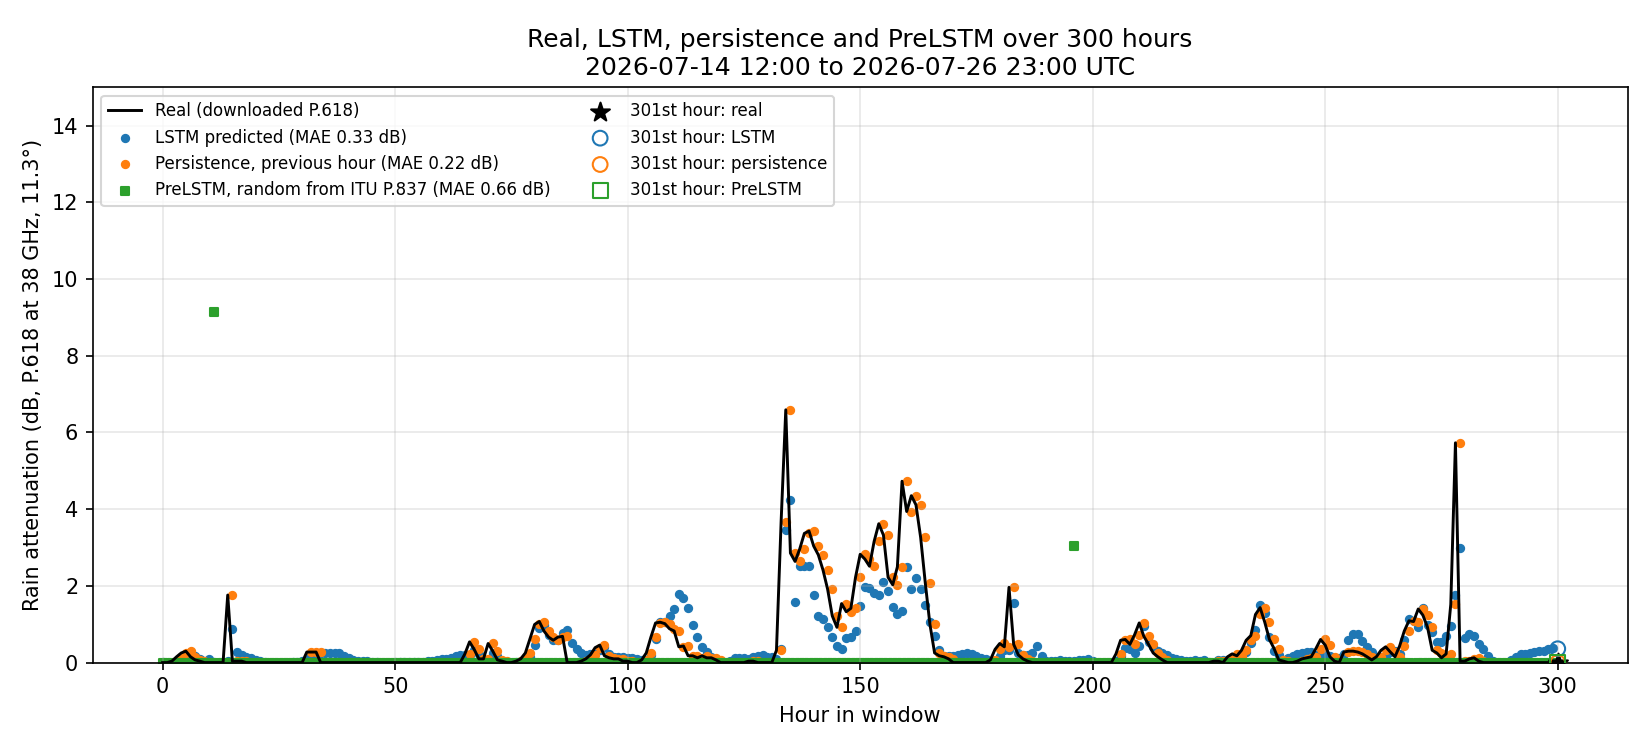
\includegraphics[width=\linewidth]{./figures/lstm_forecast_2026.png}
\caption{Real, LSTM, persistence and PreLSTM over a 300-hour window in July 2026, the window with the most rain. Real: observed hourly attenuation from the downloaded precipitation (P.838 and P.618 method, gateway geometry). LSTM: one-hour-ahead forecast. Persistence: previous hour's value. PreLSTM: random hourly rain rates drawn from the ITU-R P.837 statistics for Delhi, converted with P.618; this is a synthetic baseline with no observed data. Star and open markers show the 301st hour.}
\label{fig:lstm-2026}
\end{figure}

\subsection{Motivation: Why DRL?}
\label{sec:lstm-dqn-motivation}

The spatial SINR heterogeneity discovered in the static channel-model analysis (9.94\,dB variation at 50\,km driven by constellation geometry alone, Figure~\ref{fig:multinode-interference}) demonstrates that distance-only scheduling heuristics fail. A simple ``always pick max SINR'' rule cannot anticipate or adapt to the angular SINR patterns created by the 3-HAPS triangle. Moreover, when weather degrades feeder links (Section~\ref{subsec:multinode-sinr}), the network must dynamically fail-over users from one platform to another while respecting battery constraints on each HAPS node.

DRL offers a principled approach: the agent observes the current network state (SINR to each platform, battery levels, weather forecast) and learns a policy $\pi(a | s)$ that selects the best platform for each user, maximizing cumulative reward. By training on diverse scenarios (rain events, user mobility, multi-node interference), the learned policy discovers non-obvious patterns (e.g., preemptively rerouting from a well-positioned but rain-threatened link to a less ideal but stable backup) that no hand-crafted rule would capture.

\subsection{Per-User Markov Decision Process (MDP) Formulation}

The model has six actions: each of the three platforms (HAPS\_1, HAPS\_2, HAPS\_3) can serve a user directly or through a UAV relay. With N users, a centralized MDP would face $4^N$ possible joint assignments—intractable for large networks. We instead decompose into per-user MDPs: each user independently chooses a platform, and the network computes cumulative reward after all assignments.

\subsubsection{State Space}

The state vector for user~$k$ is 21-dimensional:
\begin{align}
\mathbf{s}_k &= [\text{SINR}_{k,1,2,3}, r_{k,1,2,3}, \text{SoC}_{1,2,3}, C^{\text{UAV}}_{k,1,2,3},\nonumber\\
&\quad R_{\text{rain}}, V_{\text{vis}}, t_{\text{hour}}, \hat{A}_{t}, \dots, \hat{A}_{t+5} ]
\label{eq:state-vector}
\end{align}
where $C^{\text{UAV}}_{k,p}$ is the UAV-relay capacity of platform $p$ for user $k$ (bits/s/Hz, from Section~\ref{sec:relay-path-analysis}), and $\hat{A}_{t+h-1}$, $h=1,\dots,6$, are the six LSTM forecasts of the feeder rain attenuation for hours $t$ to $t+5$, all issued at hour $t-1$ and normalized by 100\,dB, so no rain of hour $t$ enters the state.

\noindent \textbf{Feature Definitions}
(cross-referenced to the static channel-model analysis):

\begin{itemize}\setlength{\itemsep}{0pt}
  \item $\text{SINR}_{k,p}$: Downlink SINR at user $k$ from platform $p$ (dB). The static channel-model analysis measured $[-11.3, +7.3]$~dB across the 100~km footprint (Fig.~\ref{fig:multinode-interference}); bounds $[-20, +30]$~dB provide headroom for edge cases.
  \item $r_{k,p}$: Horizontal distance user~$k$ to platform~$p$ (km). Range $[0, 100]$~km covers service footprint (§~II).
  \item $\text{SoC}_p$: Battery state-of-charge platform~$p$ (\%). Observed by all users; range $[0, 100]\,\%$ (empty to full).
  \item $R_{\text{rain}}$: Rainfall rate (mm/h). Range $[0, 50]$~mm/h (rare events).
  \item $V_{\text{vis}}$: Visibility (m). Range $[0, 10]$~km (fog/clear).
  \item $t_{\text{hour}}$: Time-of-day (normalized). Range $[0, 1]$ maps 0~$\to$~midnight, 0.5~$\to$~noon.
\end{itemize}

\textbf{Normalisation bounds} (the agent receives each feature divided by its bound and clipped to $[0,1]$; negative SINR is preserved below the lower bound for outage signals):
\begin{itemize}\setlength{\itemsep}{0pt}
  \item SINR: $[-20,+30]$~dB; distance: $[0,100]$~km; SoC: $[0,100]$\,\%.
  \item UAV-relay capacity: $[0,20]$~bits/s/Hz (per platform).
  \item Rain: $[0,50]$~mm/h; visibility: $[0,10]$~km; hour: $[0,24]$~h.
  \item Forecasts $\hat{A}_{t},\dots,\hat{A}_{t+5}$: $[0,100]$~dB.
\end{itemize}

\noindent \textbf{DQN Scope} (scintillation deferred to future work):
\begin{itemize}\setlength{\itemsep}{0pt}
  \item \textbf{Included}: Deterministic SINR from constellation geometry (the static channel-model analysis); rainfall \& visibility for backhaul fade planning; battery state for load balancing
  \item \textbf{NOT included}: Tropospheric scintillation fading (Section~\ref{subsec:scintillation}) --- time-varying random process requiring LSTM forecasting (future work)
  \item \textbf{Approximation}: the DQN does not model scintillation; the P.618 fade at $p=1\%$ is $0.04$~dB at 2.1\,GHz and $0.6$~dB at 38\,GHz (Section~\ref{subsec:scintillation}), which is not a DQN input
  \item \textbf{LSTM forecaster}: predicts rain attenuation up to six hours ahead from past weather, all six horizons are used by the agent (Section~\ref{sec:lstm}); forecasting scintillation fading, which would enable adaptive fade reallocation, is future work
\end{itemize}

\textbf{Validation:} The static channel-model analysis measured SINR $\in [-11.3, +7.3]$~dB across the full 10--100~km, 24-point angular sweep (worst case at $r=75$\,km, $\theta=0^\circ$; best case at $r=10$\,km, $\theta=210^\circ$; Figure~\ref{fig:multinode-interference} and underlying spatial sweep data). Bounds $[-20, +30]$~dB lie $8.7$\,dB below and $22.8$\,dB above the observed range, for edge cases (atmospheric fading, relay paths in v2).

\subsubsection{Action Space}

Discrete action: $a_k \in \{0,\dots,5\}$. Actions $0$--$2$ are direct association with HAPS1--HAPS3; actions $3$--$5$ relay through a UAV served by HAPS1--HAPS3.

\subsubsection{Reward Function}

The reward is computed per user at each hour and then averaged over users and hours. For user $k$ with linear SINR $\gamma_k = 10^{\text{SINR}_{k,\text{dB}}/10}$ on its chosen link:
\begin{align}
r_k &= \omega_1\,T_k\,c_\mathrm{rain} + P^\mathrm{sev}_k + P^\mathrm{deg}_k \\
&\quad + \omega_2\,J_\mathrm{fair} - \omega_3\,P_\mathrm{eng} + P_\mathrm{LB},\\
T_k &= \log_2(1+\gamma_k) \quad [\text{bits/s/Hz}], \qquad c_\mathrm{rain} = 10^{-A_\mathrm{rain}/10} \in [0.05,1],\\
J_\mathrm{fair} &= \frac{(\sum_k \gamma_k)^2}{N \sum_k \gamma_k^2} \in [0,1], \qquad
P_\mathrm{eng} = \frac{1}{3}\sum_{p=1}^{3} \left(1 - \frac{\text{SoC}_p}{100}\right),
\end{align}
with $\omega_1=0.5$, $\omega_2=0.3$, $\omega_3=0.2$. Here $c_\mathrm{rain}$ is the feeder rain factor for the hour (applied to the throughput term), and $J_\mathrm{fair}$ is the Jain index over linear SINR, used only in the reward. The reported fairness is the Jain index over per-user delivered throughput, $T_k c_\mathrm{rain}$.

\noindent \textbf{Penalties} (per user, thresholds from the static channel-model analysis's SINR ranges):
\begin{itemize}\setlength{\itemsep}{0pt}
  \item Severe outage: $P^\mathrm{sev}_k = -100$ if $\text{SINR}_{k,\text{dB}} < -2$~dB, otherwise $0$.
  \item Degraded service: $P^\mathrm{deg}_k = -20$ if $-2 \le \text{SINR}_{k,\text{dB}} < 0$~dB, otherwise $0$.
  \item Low battery: $P_\mathrm{LB} = -50$ for each platform with $\text{SoC}_p < 10\,\%$ and at least one assigned user. This term is shared by all users.
\end{itemize}

\noindent \textbf{Worked example} (three users, one hour, $c_\mathrm{rain}=0.8$, all platforms at SoC 60\,\%, no low-battery term):

\begin{center}
\resizebox{\columnwidth}{!}{%
\begin{tabular}{lccccc}
\toprule
User & SINR (dB) & $\gamma_k$ & $T_k c_\mathrm{rain}$ & Penalty & $r_k$ \\
\midrule
1 & $+10$ & $10.00$ & $2.77$ & $0$ & $1.43$ \\
2 & $0$ & $1.00$ & $0.80$ & $0$ & $0.45$ \\
3 & $-3$ & $0.50$ & $0.47$ & $-100$ (outage) & $-99.72$ \\
\bottomrule
\end{tabular}}
\end{center}

\noindent Here $J_\mathrm{fair}=0.436$ and $P_\mathrm{eng}=0.40$, so the shared term is $0.3(0.436)-0.2(0.40)=0.051$. Each $r_k$ adds $0.051$ to the rows above. The hour's reward is the mean over users, $(1.43+0.45-99.72)/3=-32.6$. A single outage user dominates the mean, which is why the severe penalty is set to a large value.

\noindent \textbf{Threshold rationale:} The static channel-model analysis measured best $+7.3$~dB, average $+2.0$~dB and worst $-4.3$~dB. The penalties apply only below $0$~dB, so normal operation ($+2$ to $+7$~dB) earns no penalty.

\subsection{HAPS Battery Model}

\subsubsection{Energy Balance}

State-of-charge updated hourly:
\begin{equation}
\Delta \text{SoC} = \frac{P_{\text{solar}}(t) - (P_{\text{backhaul}} + P_{\text{payload}} + \sum_k P_{k,\text{user}})}{C_{\text{battery}}}
\label{eq:battery-balance}
\end{equation}

where: $P_{\text{backhaul}} = 500$~W (backhaul-link transmitter, HAPS-to-Gateway), $P_{\text{payload}} = 200$~W (control), $P_{k,\text{user}}$ (assigned load), $C_{\text{battery}} = 12000$~Wh.

\subsubsection{Solar Power (Diurnal Cycle)}

\textbf{Principle:} HAPS at 20~km (stratosphere, above $>99\%$ clouds). Solar independent of ground weather.

\noindent Solar irradiance (cosine profile):
\begin{equation}
I_0(t_{\text{hr}}) = \begin{cases}
600 \cos(\pi(t_{\text{hr}} - 12)/12) & 6 \le t_{\text{hr}} \le 18 \\
0 & \text{night}
\end{cases} \quad [\text{W/m}^2]
\end{equation}

\noindent Generated power:
\begin{equation}
P_{\text{solar}}(t) = 20\,\text{m}^2 \times 0.20 \times I_0(t) = 2400\,\text{W (noon)}, \, 0\,\text{W (night)}
\end{equation}

\subsubsection{Operating Thresholds}

SoC clipped to $[0, 100]\,\%$:
\begin{itemize}\setlength{\itemsep}{2pt}
  \item \textbf{Charging:} Day (6 AM--6 PM) when $P_{\text{solar}} > P_{\text{load}}$
  \item \textbf{Draining:} Night when $P_{\text{solar}} = 0$
  \item \textbf{Critical:} SoC $< 5\,\%$ $\Rightarrow$ shutdown (no service)
  \item \textbf{Penalty:} SoC $< 10\,\%$ with users $\Rightarrow$ reward $-50$ (load balancing)
\end{itemize}

\textbf{Thresholds:} SoC $\in [0,100]\,\%$. Critical: $< 5\%$ (shutdown); penalty: $< 10\%$ (overload). Agent learns to balance users across platforms to avoid over-draining during night.

\FloatBarrier

% =====================================================================
\section{Summary}
% =====================================================================

\subsection{Channel Model and Interference Characterisation}
\label{sec:channel-model-summary}

\paragraph{Propagation metrics and path-loss characterisation.}
The four core propagation metrics---HAPS free-space path loss, UAV LoS probability,
average air-to-ground path loss, and single-node SINR---are implemented and
characterised through Figures~\ref{fig:fspl_comparison}--\ref{fig:los_pl_sinr}.

\paragraph{Multi-HAPS interference and landscape effects.}
The multi-HAPS interference analysis (Figure~\ref{fig:multinode-interference}) is landscape-\emph{independent} for both the 2~GHz service link and the 38~GHz backhaul link: both tiers use pure free-space path loss with no environment-specific term, so suburban, urban, dense-urban, and high-rise environments produce numerically identical SINR (\S\ref{subsec:multinode-sinr}). Landscape instead matters for the separate, single-link 2~GHz baseline path-loss analysis (Figure~\ref{fig:los_pl_sinr}): suburban areas retain line-of-sight and sustain usable SINR to greater distances, while high-rise environments show sharp LoS/NLoS transitions and higher blockage loss.

Independent of landscape, adding multi-HAPS co-channel interference degrades the 2~GHz service link by roughly 11--17\,dB relative to the noise-only case (comparing the noise-only SNR to the interference-degraded SINR, e.g.\ $18.5\to7.3$\,dB near nadir and $9.9\to-7.4$\,dB at 50\,km; Table A.2, Figure~\ref{fig:multinode-interference}).

\noindent \textbf{Backhaul link (38 GHz) does NOT experience this penalty}: The three interfering HAPS are $\approx 65$ km from the ground Gateway, placing them far outside the 10--500 m backhaul coverage. Consequently, interference from constellation members remains well below thermal noise floor; backhaul SINR is primarily noise-limited and approximately constant at $+38$~dB, once the HAPS/Gateway directional antenna gains (\S\ref{subsec:backhaul-geometry}) are included in the link budget (Eq.~\eqref{eq:feeder-sinr},Figure~\ref{fig:sinr-feeder-link}).

\paragraph{Scintillation fading (ITU P.618 implementation).}
Figure~\ref{fig:scint_fade_depth} shows the ITU-R P.618 scintillation fade for the 38\,GHz gateway link and the 2.1\,GHz UE link. Over $p=0.01$--$10$\,\% and $10^\circ$--$90^\circ$ elevation, the fade is 0.04--1.8\,dB at 38\,GHz and 0.007--0.3\,dB at 2.1\,GHz. The 38\,GHz fade is about 0.2\,dB at zenith and 1.8\,dB at $10^\circ$ for $p=0.01$\,\%. These values replace the earlier empirical fit and its S-band (2.6--4.7\,dB) and Ka-band (7.6--13.1\,dB) fade values, which were not reproducible from P.618.

\noindent\textbf{Key Findings:}
\begin{itemize}
\item \textbf{9.94\,dB variation @ r~=~50\,km:} across the full 24-point angular sweep, SINR ranges --7.40\,dB (worst, $\theta=0^\circ$, toward I1) to +2.54\,dB (best, $\theta=210^\circ$)—vastly exceeds distance-based degradation. Note the asymmetric equilateral geometry (I1 @ $0^\circ$, I2 @ $60^\circ$) means the true best/worst angles are not the cardinal directions shown in Tables A.3a--d; see Figure~\ref{fig:app-constellation-sectors} for the good/bad sector layout.
\item \textbf{Spatial heterogeneity dominates r~$>$~30\,km:} At r~=~50\,km, 9.94\,dB spatial variation exceeds ~2--3\,dB per distance doubling.
\item \textbf{DRL scheduling necessity:} Distance-only assignment fails. Must learn angle-dependent interference patterns.
\item \textbf{Sector structure:} Good sector ($\sim$120--290$^\circ$, SINR~$>$~0\,dB); bad sector ($\sim$330--75$^\circ$, SINR~$<$~--5\,dB within roughly $345$--$60^\circ$).
\end{itemize}

\subsection{DQN Results}
\label{sec:dqn-results}

The DQN is trained on $400$ rolling 24-hour episodes drawn from 2024 and evaluated on $50$ calendar days from 2025, which are never seen during training. Five experiments are run, each with a new seed that sets the agent's initial weights and its random choices; every experiment uses the same training episodes and the same $50$ test days. Each training episode carries the real hourly rain, visibility, and time of day, the ITU-R P.618 rain loss, and the six LSTM forecasts issued at the previous hour (Section~\ref{sec:lstm}). The DQN and the baselines choose among the same six actions (direct and UAV-relay links for each HAPS). Every policy is evaluated on the same 50 days for each of five experiments. The reported Jain index is over per-user delivered throughput; the reward's fairness term uses Jain over linear SINR, as defined in the reward. Table~\ref{tab:dqn-all-policies} compares the policies, Table~\ref{tab:dqn-experiment-stats} gives the DQN's experiment-level statistics, Table~\ref{tab:dqn-paired} gives the paired comparisons, and Figure~\ref{fig:policy-comparison} shows the comparison graphically.

\begin{table}[t]
\centering
\caption{DQN hyperparameters (all values from the training code; identical for every experiment).}
\label{tab:dqn-hyper}
{\scriptsize\setlength{\tabcolsep}{3pt}
\begin{tabularx}{\columnwidth}{|>{\raggedright\arraybackslash}X|>{\centering\arraybackslash}X|}
\hline
\textbf{Setting} & \textbf{Value} \\
\hline
Network & MLP, input $\to$ 128 $\to$ 64 $\to$ 9 actions, ReLU \\
\hline
Optimiser / learning rate & Adam, $5\times10^{-4}$ \\
\hline
Loss & Smooth L1 (Huber) on the TD target \\
\hline
Discount factor $\gamma$ & 0.95 \\
\hline
Replay buffer / batch & 50{,}000 transitions / 128 \\
\hline
Gradient steps & one per environment step (one hour, all users) \\
\hline
Target network & copied every 200 gradient steps \\
\hline
Exploration & $\varepsilon$-greedy per user, from 1.0, multiplied by 0.99 per episode, floor 0.05; greedy at evaluation \\
\hline
Training episodes & 400 rolling 24-hour episodes from 2024, one pass \\
\hline
Experiments / evaluation & 5 experiments (0--4); 50 held-out 2025 days per experiment \\
\hline
\end{tabularx}}
\end{table}

\begin{table}[t]
\centering
\caption{Policy comparison on the 50 held-out 2025 days. All values are means over five experiments (standard deviation across experiments in brackets). Jain is over per-user delivered throughput. Max-SINR uses only the three direct links.}
\label{tab:dqn-all-policies}
{\scriptsize\setlength{\tabcolsep}{3pt}
\begin{tabularx}{\columnwidth}{|>{\raggedright\arraybackslash}X|>{\centering\arraybackslash}X|>{\centering\arraybackslash}X|>{\centering\arraybackslash}X|}
\hline
\textbf{Policy} & \textbf{Reward per step} & \textbf{Jain} & \textbf{Outage /50} \\
\hline
Random (all six actions) & $-40.5\,(1.7)$ & $0.563\,(0.007)$ & $16.5\,(0.4)$ \\
\hline
Max-SINR (direct only) & $-14.5\,(2.1)$ & $0.866\,(0.002)$ & $0.9\,(0.2)$ \\
\hline
Max-throughput (all six actions, no learning) & $-3.8\,(1.7)$ & $\mathbf{0.988}\,(0.000)$ & $\mathbf{0.0}\,(0.0)$ \\
\hline
\textbf{LSTM + DQN} & $\mathbf{+1.4}\,(1.0)$ & $0.981\,(0.006)$ & $\mathbf{0.0}\,(0.0)$ \\
\hline
\end{tabularx}}
\end{table}

\begin{table}[t]
\centering
\caption{LSTM + DQN across five experiments: mean, standard deviation, median, range, and 95\% confidence interval of the mean.}
\label{tab:dqn-seed-stats}
{\scriptsize\setlength{\tabcolsep}{2.5pt}
\begin{tabularx}{\columnwidth}{|>{\raggedright\arraybackslash}X|>{\centering\arraybackslash}X|>{\centering\arraybackslash}X|>{\centering\arraybackslash}X|>{\centering\arraybackslash}X|}
\hline
\textbf{Metric} & \textbf{Mean $\pm$ std} & \textbf{Median} & \textbf{Range} & \textbf{95\% CI} \\
\hline
Reward per step & $+1.40\pm0.96$ & $+1.92$ & $[0.02,\,2.21]$ & $[0.21,\,2.59]$ \\
\hline
Jain fairness (throughput) & $0.981\pm0.006$ & $0.984$ & $[0.970,\,0.984]$ & $[0.973,\,0.988]$ \\
\hline
Outage /50 & $0.0\pm0.0$ & $0.0$ & $[0,\,0]$ & $[0,\,0]$ \\
\hline
Battery SoC (\%) & $59.96\pm0.59$ & $59.95$ & $[59.07,\,60.53]$ & $[59.22,\,60.69]$ \\
\hline
\end{tabularx}}
\end{table}

\begin{table}[t]
\centering
\caption{Paired differences, LSTM + DQN minus each rule-based or random policy, per experiment (50 days each). Outage is better when lower.}
\label{tab:dqn-paired}
{\scriptsize\setlength{\tabcolsep}{2.5pt}
\begin{tabularx}{\columnwidth}{|>{\raggedright\arraybackslash\hsize=1.34\hsize}X|>{\centering\arraybackslash\hsize=0.81\hsize}X|>{\centering\arraybackslash\hsize=1.51\hsize}X|>{\centering\arraybackslash\hsize=0.70\hsize}X|>{\centering\arraybackslash\hsize=0.64\hsize}X|}
\hline
\textbf{Metric / comparison} & \textbf{Mean difference} & \textbf{95\% CI} & \textbf{$p$-value} & \textbf{Experiments} \\
\hline
Reward vs max-SINR & $+15.87$ & $[+13.6,\,+18.2]$ & $<0.001$ & $5/5$ \\
\hline
Reward vs max-throughput & $+5.17$ & $[+3.4,\,+6.9]$ & $0.001$ & $5/5$ \\
\hline
Jain vs max-SINR & $+0.115$ & $[+0.106,\,+0.124]$ & $<0.0001$ & $5/5$ \\
\hline
Jain vs max-throughput & $-0.007$ & $[-0.015,\,+0.001]$ & $0.07$ & $0/5$ \\
\hline
Outage vs max-SINR & $-0.87$ & $[-1.13,\,-0.61]$ & $0.0007$ & $5/5$ \\
\hline
Battery SoC vs max-SINR (\%) & $+0.03$ & $[-0.06,\,+0.11]$ & $0.44$ & $4/5$ \\
\hline
\end{tabularx}}
\end{table}

\begin{figure*}[t]
\centering
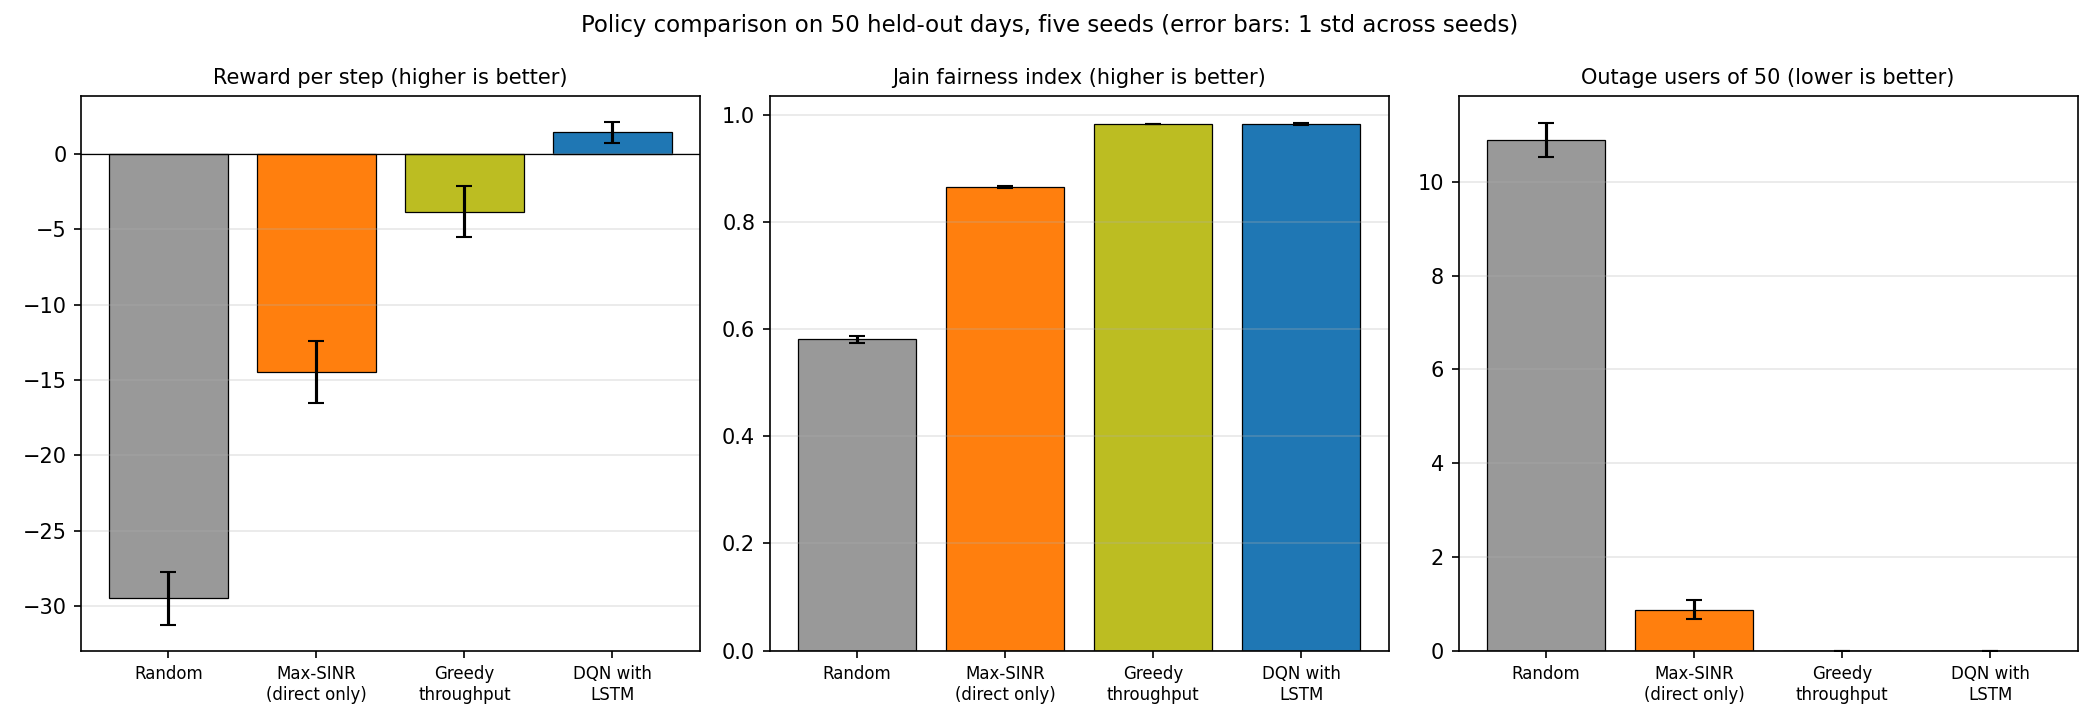
\includegraphics[width=\textwidth]{./figures/policy_comparison.png}
\caption{Policy comparison on the 50 held-out 2025 days over five experiments: reward per step (higher is better), Jain fairness over per-user throughput (higher is better), and outage users of 50 (lower is better). Bars are means over experiments; error bars are one standard deviation across experiments.}
\label{fig:policy-comparison}
\end{figure*}

\paragraph{Reward and outage.} LSTM + DQN has the highest mean reward ($+1.4$ per step) and no outage. Against the max-throughput rule, which uses the same six actions without learning, the DQN gains $5.2$ reward per step, on every experiment. Against max-SINR, which can use only the direct links, the gain is $15.9$ per step. Outage is zero for both the DQN and the max-throughput rule, and $0.9$ users on average for max-SINR (Table~\ref{tab:dqn-paired}).

\paragraph{Fairness.} The reported Jain index is over per-user delivered throughput. The DQN ($0.98$) and the max-throughput rule ($0.99$) are close, and the difference between them is not significant. Both are fairer than max-SINR ($0.87$) and random ($0.56$). The reward's own fairness term is Jain over linear SINR. It enters the reward but is not the reported measure.

\paragraph{Random and rule-based policies and weather.} Random association is worst on every metric. The random and max-SINR policies do not read the forecast or the rain, so their results depend only on the evaluation days. Their results on the synthetic PreLSTM days (50 days with hourly rain drawn from the ITU-R P.837 statistics for Delhi) agree with the real-weather results to within $0.2$ in reward. The synthetic days therefore reproduce the baseline behaviour, and they are used only as this check.

\paragraph{Limitation.} The DQN and the max-throughput rule share the same action set, so the gap between them isolates what the learned policy adds. The topology has a single ground gateway serving the network, and sharing of that gateway is not modelled. All weather data are for one site (Delhi, 28.61\,N, 77.21\,E), so the rain statistics and the forecast skill may not transfer to other climates.

% =====================================================================
\paragraph{Future work: spatio-temporal forecasting.} The forecaster uses only the target site's past weather, so its skill is limited to that site. A natural extension is a spatio-temporal graph model (for example DCRNN, T-GCN or Graph WaveNet): each region is a node, neighbouring regions are linked, an LSTM runs over time at each node, and the edge weights are learned to estimate how much each neighbour contributes to the target. This would draw on regions from the coast to the desert and from the Himalayas to the plains. It needs time series for every node, a check that the learned edges are physically plausible, and a comparison with the present LSTM, persistence and same-hour average on the same hours. Any change to the forecast would also require retraining the DQN.

\section{Conclusion}
\label{sec:conclusion}
% =====================================================================

This document characterised the HAPS-UAV-Gateway air-to-ground channel
across three link types -- the 2\,GHz HAPS$\rightarrow$UE service link,
the 38\,GHz HAPS$\rightarrow$Gateway backhaul link, and the two-hop
HAPS$\rightarrow$UAV$\rightarrow$UE relay link (whose first, 38\,GHz hop is
the feeder link) -- and used that channel
model to both characterise multi-HAPS interference (\S\ref{sec:channel-model-summary})
and train a DQN agent for user-platform association (\S\ref{sec:dqn-results}).

\paragraph{Channel model.} Spatial SINR heterogeneity, not distance alone,
dominates service-link quality: a 9.94\,dB spread at a fixed 50\,km radius
(\S\ref{sec:channel-model-summary}) exceeds the degradation from doubling distance.
The backhaul link remains noise-limited and largely unaffected by constellation
geometry, while scintillation adds a frequency- and elevation-dependent
fade on both links (\S\ref{subsec:scintillation}).

\paragraph{Relay path analysis.} The topology's actual relay route,
HAPS$\rightarrow$UAV$\rightarrow$UE (\S\ref{sec:relay-path-analysis}), was
evaluated as an alternative to the direct service link. The access hop (UAV$\rightarrow$UE) is
$\approx+33$\,dB SINR at 500\,m because the UAV hovers close to the user it serves. The feeder hop
(HAPS$\rightarrow$UAV, 38\,GHz) has antenna gains $G_h=13.8$\,dBi and $G_u=30.7$\,dBi
(\cite{karaman2025haps,anim2021uav}); its SINR is $+37.6$\,dB at nadir and $+22.6$\,dB at 100\,km, well above the
$+8$\,dB design floor (Eq.~\eqref{eq:sinr-min-design}, derived from the 16-QAM/CQI-7 minimum-MCS SINR at 10\% BLER~\cite{3gpp_ts38214}
plus a 3\,dB margin). The direct HAPS$\rightarrow$UE link, which shares the 2\,GHz band with the other two HAPS, falls from
$+7.3$\,dB to $-9.1$\,dB. The decode-and-forward end-to-end capacity is $11.1$\,bits/s/Hz at nadir and $7.5$\,bits/s/Hz at 100\,km,
against the direct link's $2.7$ and $0.5$\,bits/s/Hz. The relay therefore outperforms
the direct link at every distance in this model. A practical implication for
deployment: the 38\,GHz feeder hop's rain and scintillation losses both grow
sharply as elevation drops with increasing HAPS--UAV distance (\S\ref{subsec:scintillation}),
so keeping the UAV relay near the HAPS nadir -- at as high an elevation angle as
feasible -- limits this slant-path penalty, even though the feeder SINR stays
above the design floor across the full range modelled here. Near-nadir
positioning also tends to place the UAV away from the interferer-facing
sector (\S\ref{sec:channel-model-summary}), but this is not a single clean
optimization: each HAPS could simultaneously be a serving node (near-nadir,
low-loss, for its own users) and an interferer (for the other two HAPS'
users), so jointly optimizing UAV/HAPS positioning across both roles at
once, rather than each in isolation, is left to future work.
DQN association agent (\S\ref{sec:lstm-dqn-motivation}) can route traffic through the UAV relay, as one of its six actions.

\paragraph{Learned association.} The LSTM-fed DQN agent (\S\ref{sec:dqn-results}) has the highest reward of the policies tested on the held-out 2025 days ($+1.4$ per step, against $-3.8$ for a max-throughput rule over the same six actions and $-14.5$ for max-SINR), with zero outage and per-user throughput fairness close to the max-throughput rule (Jain $0.98$ against $0.99$; the difference is not significant). The reward advantage over the max-throughput rule holds on all five experiments. Max-SINR assumes the SINR to every platform is known at decision time, which a deployed system must measure, and it cannot use the relays. Two
directions for future work follow: (1) adding a fairness-aware reward to test whether the learned policy trades fairness for throughput, and testing on harder (e.g.\ rain- or
mobility-heavy) scenarios, and (2) learning how the relay options are used across user distances, since the relay outperforms the direct link at every
distance in this model, so the learned
policy decides when relaying is
worthwhile as a function of user distance.

\section{Abbreviations}

\begin{tabular}{ll}
\textbf{ABS} & Aerial Base Station \\
\textbf{AGL} & Above Ground Level \\
\textbf{CDF} & Cumulative Distribution Function \\
\textbf{DRL} & Deep Reinforcement Learning \\
\textbf{DQN} & Deep Q-Network \\
\textbf{FDMA} & Frequency Division Multiple Access \\
\textbf{FSPL} & Free-Space Path Loss \\
\textbf{GW} & Gateway \\
\textbf{HAPS} & High-Altitude Platform Station \\
\textbf{ITU} & International Telecommunication Union \\
\textbf{K-band} & 18--27 GHz (ITU-R P.618 scintillation model) \\
\textbf{Ka-band} & 27--40 GHz (Scaled from K-band via $(f/20)^{0.7}$) \\
\textbf{LoS} & Line-of-Sight \\
\textbf{LSTM} & Long Short-Term Memory \\
\textbf{LWC} & Liquid Water Content \\
\textbf{MDP} & Markov Decision Process \\
\textbf{MLP} & Multi-Layer Perceptron \\
\textbf{MVP} & Minimum Viable Product \\
\textbf{NLoS} & Non-Line-of-Sight \\
\textbf{PDF} & Probability Density Function \\
\textbf{PL} & Path Loss \\
\textbf{RH} & Relative Humidity \\
\textbf{SINR} & Signal-to-Interference-plus-Noise Ratio \\
\textbf{SoC} & State of Charge (Battery) \\
\textbf{TDMA} & Time Division Multiple Access \\
\textbf{TD} & Temporal Difference \\
\textbf{UAV} & Unmanned Aerial Vehicle \\
\textbf{UTD} & Uniform Theory of Diffraction \\
\end{tabular}

\section{References}

% =====================================================================
%\renewcommand{\refname}{}
\begin{thebibliography}{30}

% === ITU-R Recommendations (Propagation) ===
\bibitem{itu_m2101}
ITU-R Recommendation M.2101-0, ``Characteristics of High Altitude Platform Stations
(HAPS) operating in the stratosphere,'' 2017.
Available: \url{https://www.itu.int/rec/R-REC-M.2101/latest/}

\bibitem{itu_m2106}
ITU-R Recommendation M.2106-1, ``Characteristics of High Altitude Platform Stations
(HAPS) operating in the stratosphere,'' 2012.
Available: \url{https://www.itu.int/rec/R-REC-M.2106/latest/}

\bibitem{itu_p530}
ITU-R Recommendation P.530-17, ``Propagation data and prediction methods required
for the design of terrestrial line-of-sight systems,'' 2021.
Available: \url{https://www.itu.int/rec/R-REC-P.530/latest/}

\bibitem{itu_p618}
ITU-R Recommendation P.618-13, ``Propagation data and prediction methods for the
design of Earth-space telecommunication systems,'' 2021.
Available: \url{https://www.itu.int/dms_pubrec/itu-r/rec/p/R-REC-P.618-13-202108-S!!PDF-E.pdf}
[Covers rain attenuation reduction factors, slant-path geometry, scintillation model]

\bibitem{itu_p838}
ITU-R Recommendation P.838-3, ``Specific attenuation model for rain for use in
prediction methods,'' 2005.
Available: \url{https://www.itu.int/dms_pubrec/itu-r/rec/p/R-REC-P.838-3-200503-S!!PDF-E.pdf}
[Annex 1: frequency-dependent rain coefficients $k(f)$, $\alpha(f)$]

\bibitem{itu_p676}
ITU-R Recommendation P.676-12, ``Attenuation by atmospheric gases and related
effects,'' 2021.
Available: \url{https://www.itu.int/dms_pubrec/itu-r/rec/p/R-REC-P.676-12-202112-S!!PDF-E.pdf}
[Section 3.1.2: O$_2$ resonance (59.8 GHz, 118.75 GHz); Section 3.2.1: H$_2$O resonance (22.235 GHz)]

\bibitem{itu_p840}
ITU-R Recommendation P.840-6, ``Attenuation due to clouds and fog,'' 2021.
Available: \url{https://www.itu.int/dms_pubrec/itu-r/rec/p/R-REC-P.840-6-202101-I!!PDF-E.pdf}
[Liquid water content model for fog/cloud attenuation]

\bibitem{itu_p835}
ITU-R Recommendation P.835-7, ``Reference standard atmospheres,'' 2017.
Available: \url{https://www.itu.int/dms_pubrec/itu-r/rec/p/R-REC-P.835-7-201703-I!!PDF-E.pdf}

\bibitem{itu_p836}
ITU-R Recommendation P.836-5, ``Surface water vapour statistics,'' 2017.
Available: \url{https://www.itu.int/dms_pubrec/itu-r/rec/p/R-REC-P.836-5-201703-I!!PDF-E.pdf}

\bibitem{itu_p837}
ITU-R Recommendation P.837-7, ``Characteristics of precipitation for propagation
modelling,'' 2017.
Available: \url{https://www.itu.int/dms_pubrec/itu-r/rec/p/R-REC-P.837-7-201706-I!!PDF-E.pdf}

\bibitem{itu_p1410}
ITU-R Recommendation P.1410-5, ``Propagation data and prediction methods for the
design of terrestrial broadband radioaccess systems operating in a frequency range
from 3 to 60 GHz,'' 2021.
Available: \url{https://www.itu.int/rec/R-REC-P.1410/latest/}
[Elevation-angle-dependent LoS probability baseline]

% === 3GPP / NTN Standards ===
\bibitem{3gpp_ts38821}
3GPP TR 38.821, ``Study on New Radio (NR) and its Evolution for Non-Terrestrial
Networks (NTN),'' Release 17, September 2022 (study report; background only).
Available: \url{https://www.3gpp.org/DynaReport/38821.htm}

\bibitem{3gpp_ts38214}
3GPP TS 38.214, ``NR; Physical layer procedures for data,'' Release 16, 2021.
Available: \url{https://www.3gpp.org/DynaReport/38214.htm}
[CQI/MCS-to-SINR design reference: CQI index 1 (QPSK, code rate 78/1024)
requires $\mathrm{SINR}\approx-6$\,dB; CQI index 7 (16-QAM, code rate
378/1024) requires $\mathrm{SINR}\approx+5$\,dB; CQI index 15 (256-QAM, code
rate 948/1024) requires $\mathrm{SINR}>+22$\,dB, all at the standard 10\% first-
transmission BLER target.]

\bibitem{karaman2025haps}
B.~Karaman, I.~Basturk, F.~Kara, E.~Zeydan, E.~A.~Beyazit, S.~Taskin,
E.~Bj\"ornson, and H.~Yanikomeroglu, ``On-Demand HAPS-Assisted Communication
System for Public Safety in Emergency and Disaster Response,'' \emph{IEEE
Commun. Mag.}, 2025. arXiv:2507.09153.
[Ka-band (30\,GHz) HAPS backhaul link budget, Table I: Tx power 43.2\,dBm, Tx
antenna gain 13.8\,dBi, Rx (VSAT) antenna gain 39.7\,dBi -- used here as the
literature-typical antenna-gain basis for this document's 38\,GHz
feeder-style links, \S\ref{sec:relay-path-analysis}.]

\bibitem{anim2021uav}
K.~Anim, J.-N.~Lee, and Y.-B.~Jung, ``High-Gain Millimeter-Wave Patch Array
Antenna for Unmanned Aerial Vehicle Application,'' \emph{Sensors}, vol.~21,
no.~11, p.~3914, 2021. DOI: 10.3390/s21113914
[UAV-mountable $32\times32$ mmWave patch array antenna, realized gain
30.7--32.8\,dBi at 25.4--26.9\,GHz -- basis for this document's UAV-side
receive antenna gain on the HAPS\,$\rightarrow$\,UAV hop,
\S\ref{sec:relay-path-analysis}.]

\bibitem{3gpp_ts36104}
3GPP TS 36.104, ``Evolved Universal Terrestrial Radio Access (E-UTRA); Base Station
(BS) Radio Transmission and Reception,'' Release 16, December 2021.
Available: \url{https://www.3gpp.org/DynaReport/36104.htm}
[LTE channel bandwidth specifications; 20 MHz service-link allocation]

% === Peer-Reviewed Publications ===
\bibitem{arani2023}
A.~H. Arani, P.~Hu, and Y.~Zhu, ``HAPS-UAV-Enabled Heterogeneous Networks: A Deep
Reinforcement Learning Approach,'' \emph{IEEE Open J. Commun. Soc.}, vol.~4,
pp.~1745--1760, 2023.
DOI: 10.1109/OJCOMS.2023.3294598

\bibitem{holispechac2008}
J.~Holis and P.~Pechac, ``Elevation Dependent Shadowing Model for Mobile
Communications via High Altitude Platforms in Built-up Areas,'' \emph{IEEE
Trans. Antennas Propag.}, vol.~56, no.~4, pp.~1078--1084, Apr. 2008.
DOI: 10.1109/TAP.2008.919209
[Building-blockage LoS probability series; environment parameters (Table I): $(\alpha, \beta, \xi)$ for suburban/urban/dense-urban/high-rise]

\bibitem{bakambekova2024}
A.~Bakambekova, N.~Kouzayha, and T.~Al-Naffouri, ``On the Interplay of Artificial
Intelligence and Space-Air-Ground Integrated Networks: A Survey,'' \emph{IEEE Open
J. Commun. Soc.}, vol.~5, pp.~4613--4673, 2024.

% === Regulatory / Industry Standards ===
\bibitem{ecc_report_156}
European Communications Committee (ECC), ``Minimum performance characteristics
for spectrum sharing between Fixed Satellite Service (FSS) and other services,''
ECC Report 156, April 2011 (updated December 2014).
Available: \url{https://www.ecc.cept.org/ecc/documents/ecc-reports/}
[Spectrum-sharing guidance; rain attenuation margins at Ka-band]

\bibitem{ecc_rec_04_05}
European Communications Committee (ECC), ``Radio Frequency Channel Arrangements for
Fixed Service Systems Operating in the Bands 6--7 GHz and 36--40 GHz,''
ECC Recommendation (04)05, Strasbourg, France.
[Ka-band channelization for backhaul systems]

% === SINR and Signal Analysis ===
\bibitem{itu_p618}
ITU-R, ``Propagation data and prediction methods for the design of Earth-space
telecommunication systems,'' Recommendation ITU-R P.618--13, Geneva, Switzerland, 2017.
[SINR definition $\gamma = C/(N+I)$, rain attenuation, feeder-link margins]

\bibitem{goldsmith2005}
A.~Goldsmith, \emph{Wireless Communications}, Cambridge University Press, 2005.
[Multi-user SINR in linear domain; noise and interference are additive in linear scale, not dB]

\bibitem{3gpp_ntn}
3GPP, ``Study on New Radio (NR) and its evolution for Non-Terrestrial Networks,''
Technical Report 3GPP TR 38.821, Release 16, April 2020.
[Multi-beam HAPS interference model: $\mathrm{SINR}_k = P_{\mathrm{serving}} \cdot G_k / (N_0 + \sum P_i \cdot G_{i,k})$]

% === Implementation Libraries ===
\bibitem{itur_package}
I.~Portillo-Ramirez, ``itur: Python implementation of ITU-R P recommendations,''
GitHub, 2024. Available: \url{https://github.com/iportillo/itur}
[Bundled ITU-R models for rain, fog, gas, scintillation]

% === Deep Reinforcement Learning (Phase 2) ===
\bibitem{mnih2015dqn}
V.~Mnih, K.~Kavukcuoglu D.~Silver, A.~A.~Rusu, J.~Veness, G.~Bellemare,
A.~Graves, M.~Riedmüller, A.~K.~Fidjeland, G.~Ostrovski, S.~Petersen,
C.~Beattie, A.~Sadik, I.~Antonoglou, H.~King, D.~Kumaran, D.~Wierstra,
S.~Legg, and D.~Hassabis, ``Human-level control through deep reinforcement
learning,'' \emph{Nature}, vol.~529, pp.~529--533, 2015.
[Foundational DQN algorithm: experience replay, target networks, Q-learning]

\bibitem{sutton2018rl}
R.~S.~Sutton and A.~G.~Barto, \emph{Reinforcement Learning: An Introduction},
2nd~ed. Cambridge, MA: MIT Press, 2018.
[MDP theory, value functions, policy gradient methods; Chapter 6: Q-learning]

\bibitem{schulman2017ppo}
J.~Schulman, F.~Wolski, P.~Dhariwal, A.~Radford, and O.~Klimov,
``Proximal policy optimization algorithms,'' arXiv preprint arXiv:1707.06347, 2017.
[Policy-gradient alternative to DQN; higher sample complexity for discrete actions]

\bibitem{goldsmith2005wireless}

\bibitem{mnih2015human}
V.~Mnih et~al., ``Human-level control through deep reinforcement learning,''
\textit{Nature}, vol.~529, no.~7587, pp.~529--533, Feb.~2015.

\bibitem{jain1984quantitative}
R.~K.~Jain et~al., ``A quantitative measure of fairness and discrimination for resource allocation in shared computer systems,''
\textit{arXiv preprint arXiv:cs/9809099}, 1984.

\bibitem{sutton2018reinforcement}
R.~S.~Sutton and A.~G.~Barto, \textit{Reinforcement Learning: An Introduction},
2nd~ed. MIT Press, 2018.
A.~Goldsmith, \emph{Wireless Communications}, 2nd~ed. Cambridge University Press, 2005.
[Chapter 3: SINR computation in linear domain, not dB; multi-user interference]


\bibitem{wrc19}
ITU, Final Acts of the World Radiocommunication Conference (WRC-19), agenda item 1.4 (HAPS): identification of 31--31.3\,GHz and 38--39.5\,GHz for HAPS use, and of 47.2--47.5\,GHz and 47.9--48.2\,GHz. [Verify resolution number and footnote wording against the Radio Regulations.]

\bibitem{3gpp_ts38101_5}
3GPP TS 38.101-5, ``NR; User Equipment (UE) radio transmission and reception; Part 5: Satellite access Radio Frequency (RF) and performance requirements.'' Band n256 (FDD): 1980--2010\,MHz uplink, 2170--2200\,MHz downlink. [Verify release number.]

\end{thebibliography}


\end{document}

